%% pasner_thesis.tex 11/14/2018
%% Modified by Jacob M. Pasner
%% Copyright (C) 1988-2004 Daniel Gildea, BBF, Ethan Munson.
%
% This work may be distributed and/or modified under the
% conditions of the LaTeX Project Public License, either version 1.3
% of this license or (at your option) any later version.
% The latest version of this license is in
%   http://www.latex-project.org/lppl.txt
% and version 1.3 or later is part of all distributions of LaTeX
% version 2003/12/01 or later.
%
% This work has the LPPL maintenance status "maintained".
% 
% The Current Maintainer of this work is Daniel Gildea.

\documentclass[11pt]{ucthesis}
\def\dsp{\def\baselinestretch{2.0}\large\normalsize}
\dsp

% Feynman Diagram Stuff
\RequirePackage{luatex85}
\usepackage{tikz-feynman}
\tikzfeynmanset{compat=1.1.0} 

% Declare usepackages here:
\usepackage{lineno}
\usepackage{color}   % May be necessary if you want to color links
\usepackage{hyperref} % Makes Chapter titles into links
\usepackage{amsmath}
\usepackage{booktabs}
\usepackage{bm}
\usepackage{caption,subcaption,epsfig}
\usepackage{cleveref}
\hypersetup{
  colorlinks=true, % set true if you want colored links
  linktoc=all,     % set to all if you want both sections and subsections linked
  citecolor=black,
  filecolor=black,
  linkcolor=black, % choose some color if you want links to stand out
  urlcolor=black
}

\linenumbers

\setlength{\parindent}{0pt} % no indentation
\setlength{\parskip}{2ex} % larger space between paragraphs

% Definitions for using atlas latex
\newcommand*{\ATLASLATEXPATH}{atlaslatex/latex/}
\usepackage[jetetmiss,particle,misc]{atlaslatex/latex/atlasphysics}
\usepackage[backend=biber,sorting=none,backref=true]{biblatex}

% Define biliography resources for lookup by biber
\addbibresource{atlaslatex/bib/ATLAS-useful.bib}
\addbibresource{atlaslatex/bib/ATLAS-errata.bib}
\addbibresource{atlaslatex/bib/ATLAS.bib}
\addbibresource{atlaslatex/bib/CMS.bib}
\addbibresource{atlaslatex/bib/ConfNotes.bib}
\addbibresource{atlaslatex/bib/PubNotes.bib}
\addbibresource{pasner_thesis.bib}


\begin{document}

% Declarations for Front Matter

\title{An Inclusive Search for the decay of a Boosted Higgs boson in the $H
\rightarrow$ \MakeLowercase{$b\overline{b}$} channel with the ATLAS detector}
\author{Jacob Martin Pasner}
\degreeyear{2019}
\degreemonth{October}
\degree{DOCTOR OF PHILOSOPHY}
\chair{Professor Jason Nielsen}
\committeememberone{Professor Abraham Seiden}
\committeemembertwo{Professor Michael Hance}
\numberofmembers{3} %% (including chair) possible: 3, 4, 5, 6
\deanlineone{Dean Lori Kletzer}
\deanlinetwo{Vice Provost and Dean of Graduate Studies}
\deanlinethree{}
\field{Particle Physics}
\campus{Santa Cruz}

\begin{frontmatter}

\maketitle
\copyrightpage

\tableofcontents
\listoffigures
\listoftables

\begin{abstract}

A search for high-momentum Higgs bosons, produced with an associated jet and
decaying to bottom quark pairs, is conducted using an integrated luminosity of
$80.5~\ifb$ of proton-proton collisions at $\sqrt{s} = 13~\TeV$ collected
with the ATLAS detector at the Large Hadron Collider.  The search for $H
\rightarrow b\bar{b}$ is of particular importance, as current measurements of
this decay channel contain large uncertainties and have not yet established
evidence for the gluon-gluon fusion and vector boson fusion Higgs boson
production modes. This is the first time this analysis has been performed with
$\sqrt{s} = 13~\TeV$ at ATLAS and represents an important advancement in the use
of boosted jet techniques including implementation of the Variable Radius jet
algorithm.  Furthermore, a novel $t\bar{t}$ control region strategy is
implemented to correct the mismodeling of its normalization and is shown to
constrain the associated large JES and JMR systematic uncertainties. For the
Standard Model Higgs boson, the observed signal strength is $\mu_{H} = 5.8 \pm
3.1~\mathrm{(stat.)} \pm 1.9~\mathrm{(syst.)} \pm 1.7~\mathrm{(theo.)}$, which
is 1.6 standard deviations higher than the background-only hypothesis, with an
expected sensitivity of $0.28\sigma.$


\end{abstract}

\begin{dedication}
\null\vfil
{\large
\begin{center}
Dedication\\\vspace{12pt}
Dedication\\\vspace{12pt}
Dedication
\end{center}}
\vfil\null
\end{dedication}


\begin{acknowledgements}

\label{sec:acknowledgements}

I would like to thank my committee for their dutiful efforts to make this
document one I can be proud of for the rest of my life.  Furthemore, I would
like to thank the SCIPP collaboration and UCSC Physics Department for their
support in both academic and personal arenas.


\end{acknowledgements}

\end{frontmatter}


\chapter{Introduction} \label{sec:intro}
As children we are fascinated with the natural world that surrounds us.  How
was it made? What is it made of?  Why is it made of that? Where did it come
from?  When was it made? These questions follow some of us into adulthood and
lead to the study of the fundamental interactions of the Universe, the pursuit
of the building blocks of reality.  For the past century, experiments of
increasing size and complexity have probed higher energies and smaller
distances to answer these questions out of the pure desire to know the unknown.
The results of these experiments have been interpreted and used to build the
most predictive and successful theory across all of science - the Standard
Model (SM) of particle physics. At the current state-of-the-art facility, the
Large Hadron Collider (LHC), an international team of scientists and engineers
continue this legacy of discovery.  There, protons are smashed together at
energies not seen since the birth of the Universe some 13.8 billion years ago
and the results are analyzed to answer the outstanding questions of our time.

In 2012 the discovery of a Higgs-like boson at CERN by the ATLAS and CMS
collaborations answered one of these outstanding questions, namely: What is the
origin of mass for particles in the SM \cite{Aad:2012tfa,Chatrchyan:2012xdj}?
This was a major triumph for both the theoretical and experimental particle
physics communities and resulted in the Nobel Prize in Physics being awarded to
Francois Englert and Peter W. Higgs for their contributions to the Higgs Boson
theory. However, the properties of this new particle are still under
verification and new physics could be lurking in the large uncertainties of
current observations of the SM Higgs boson.  In particular, the coupling
strength of the Higgs boson to bottom quarks ($H \rightarrow b\bar{b}$) was
only observed in 2018 and still contains a large uncertainty on the
measurement. Furthermore, the $H \rightarrow b\bar{b}$ decay mode has yet to be
observed for the vector boson fusion and gluon-gluon fusion production
mechanisms.  Finally, there is evidence that new physics could be accessible in
analysis observing highly boosted Higgs bosons produced via gluon-gluon fusion.
Thus, the goal of this analysis is to make a direct measurement of the coupling
of the Higgs to bottom quarks, with particular focus on the observation in the
gluon-gluon fusion and vector boson fusion production modes. 

\Cref{part:theory} of this dissertation describes the Standard Model of
particle physics including the Higgs mechanism and motivates the search for a
highly boosted $H \rightarrow b\bar{b}$. \Cref{part:experiment} describes both
the LHC and the ATLAS detector located at CERN. Lastly, \Cref{part:HbbISR}
presents the data analysis and the Boosted Higgs boson measurement results.


\part{Theoretical Motivations and the Standard Model}
% The Standard Model and Beyond

\chapter{The Standard Model and Beyond} \label{chap:standard_model}

The Standard Model (SM) of Particle Physics is humanities best "guess" at the
force laws that describe the observed behavior of all particles in our
universe. Its formulation is a collection of Quantum Field Theories (QFT) that
describe the following interactions of elementary matter in Nature: the
electromagnetic force, the weak nuclear force and the strong nuclear force.
Gravity is noticeably absent as currently there is no viable quantum theory for
observed gravitational effects.  The Glashow-Salam-Weinberg (GSW) theory of Quantum
Electrodynamics (QED) describes the electromagnetic and weak forces, while
Quantum Chromodyanmics (QCD) describes the strong force.  These theories form
the following symmetry group of the Standard Model.

\begin{equation} \label{eq:standardmodel:symmetry_group}
  \underbrace{\text{SU}_\text{C}(3)}_\text{QCD} \otimes
\underbrace{\text{SU}_\text{L}(2) \otimes \text{U}_\text{Y}(1)}_\text{GSW}.
\end{equation}

The gauge principle states that the SM Lagrangian and its predictions must be
invariant under local transformations using an operator from any of these
constituent groups.  Thus, any theory must only include transformations and
terms that maintain the local invariance of the complete Lagrangian.  In
particular, this requirement was violated by any attempt to include an explicit
mass term for the Gauge Bososns of QED and for all fermions.  Around 1960 a
possible solution to this lack of mass was proposed in the form of the
spontaneous breaking of the ElectroWeak symmetry, now known as the Higgs
mechanism.  In the following sections I will go into more detail about the
Lagrangian formalism of the Standard Model, QCD, QED and this recently verified
Higgs Mechanism.

\section{The Standard Model} \label{sec:theory:standardmodel}

At the turn of the 20th century, humanities understanding of the constituent
matter of the universe was limited to what could be seen with microscopes and
implied from the observations of light and electricity, giving evidence for
both the photon and the electron.  In the first half of the century the field
of subatomic physics was discovered with Rutherfords 1911 gold foil scattering
experiment \cite{Rutherford:1911zz} followed by the observation of
the wave-particle duality of nature with Compton's scattering experiment in
1923 \cite{PhysRev.21.483}. These were the first steps towards a Quantum Field
Theory representation of nature.  In the second half of the century experiments
delved deeper to discover that the nucleus contained structure thus the SM was
extended to include the complex mechanics of quarks and gluons
\cite{Fritzsch:1972jv}.  With the discovery of the Higgs in 2012, the Standard
Model has become even more firmly established as can be seen in the high level
of agreement between theory and experiment in \Cref{fig:xsection_measurements}.

\begin{figure}[!htbp]
  \begin{center}
    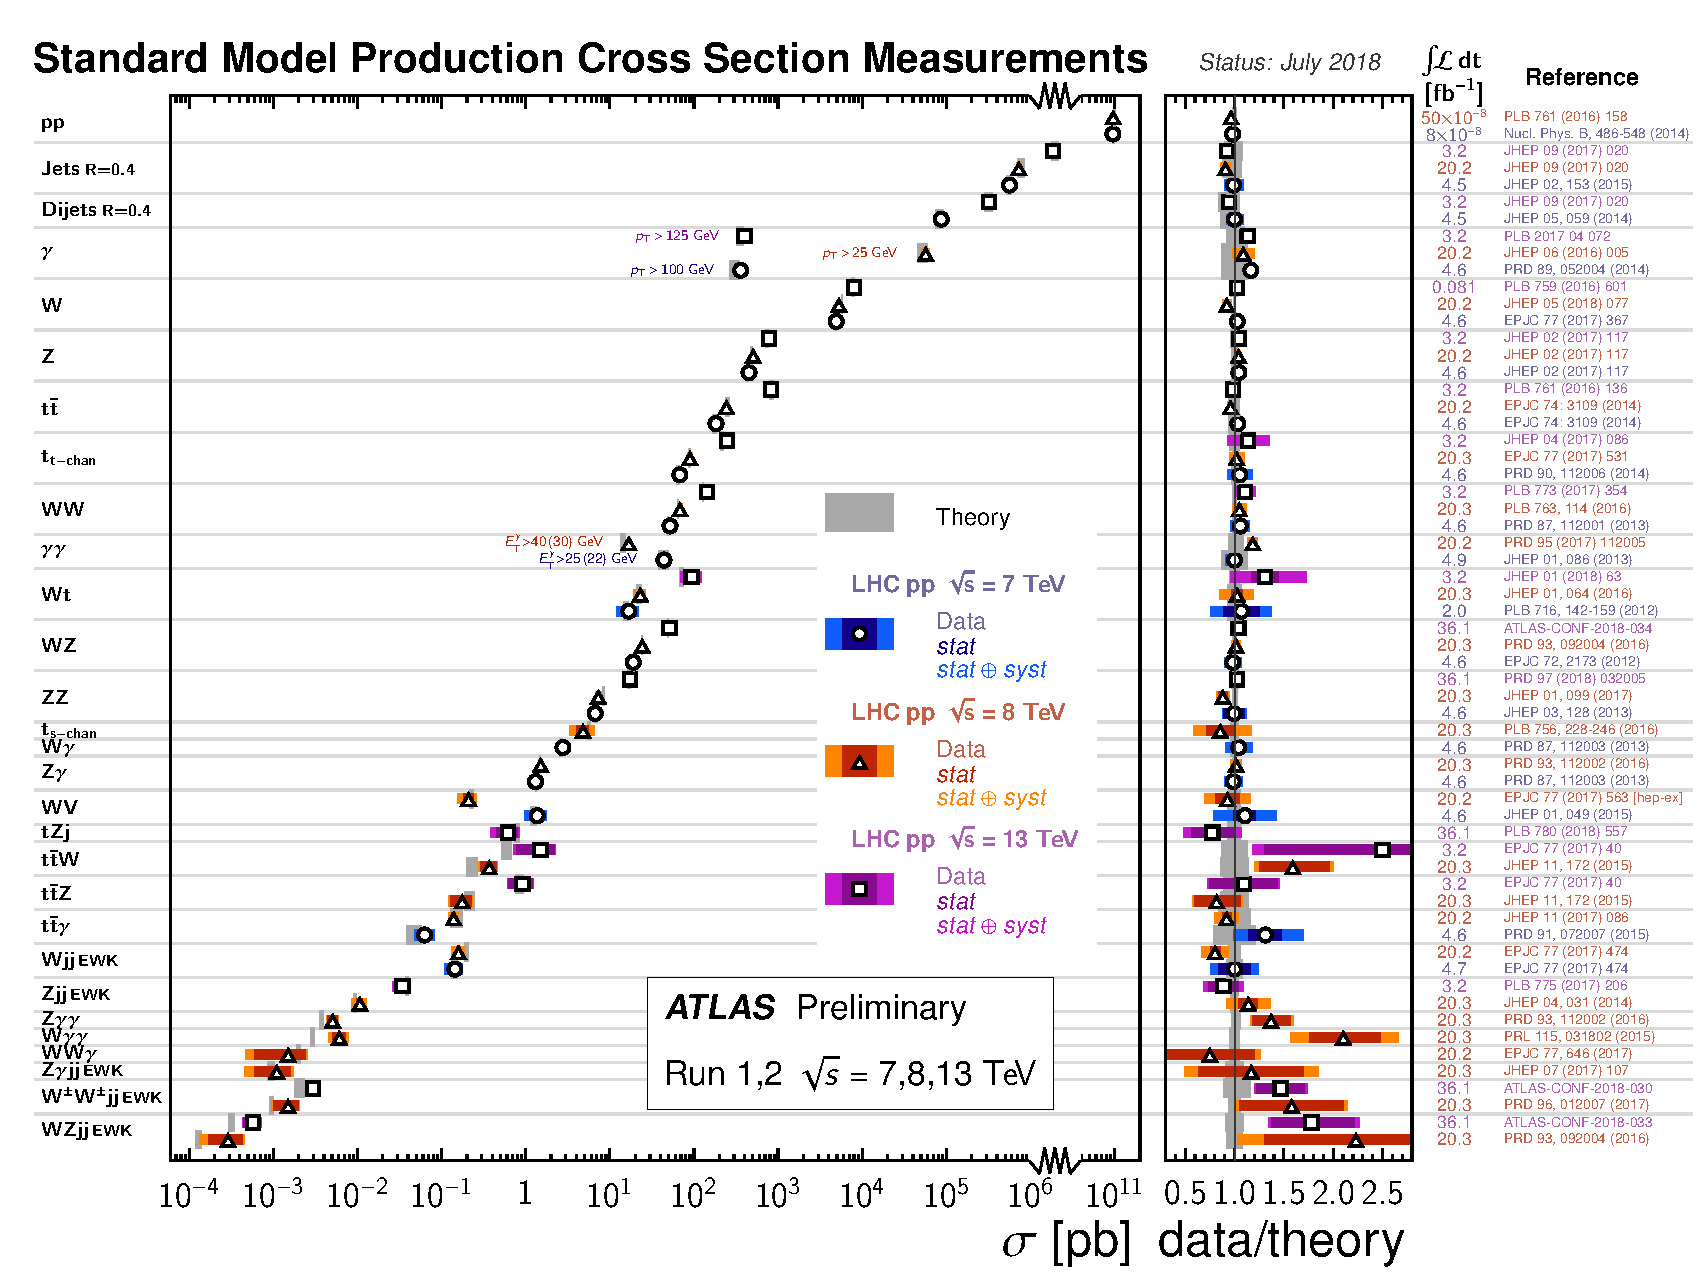
\includegraphics[width=\linewidth]{figures/theory/xsection_measurements.pdf}
\caption{ Summary of several Standard Model total and fiducial production cross
section measurements, corrected for leptonic branching fractions, compared to
the corresponding theoretical expectations \cite{StandardModelPublicResults}.
All theoretical expectations were calculated at NLO or higher. The dark-color
error bar represents the statistical uncertainty. The lighter-color error bar
represents the full uncertainty, including systematics and luminosity
uncertainties. The data/theory ratio, luminosity used and reference for each
measurement are also shown. Uncertainties for the theoretical predictions are
quoted from the original ATLAS papers. They were not always evaluated using the
same prescriptions for PDFs and scales.}
    \label{fig:xsection_measurements}
  \end{center}
\end{figure}

The QCD and GSW theories predict two classes of particles - fermions and bosons -
shown in \Cref{fig:standard_model}. These particles represent the quanta
of the quantum fields of the Standard Model and the mediators of the fundamental
forces of Nature.

\begin{figure}[!htbp]
  \begin{center}
    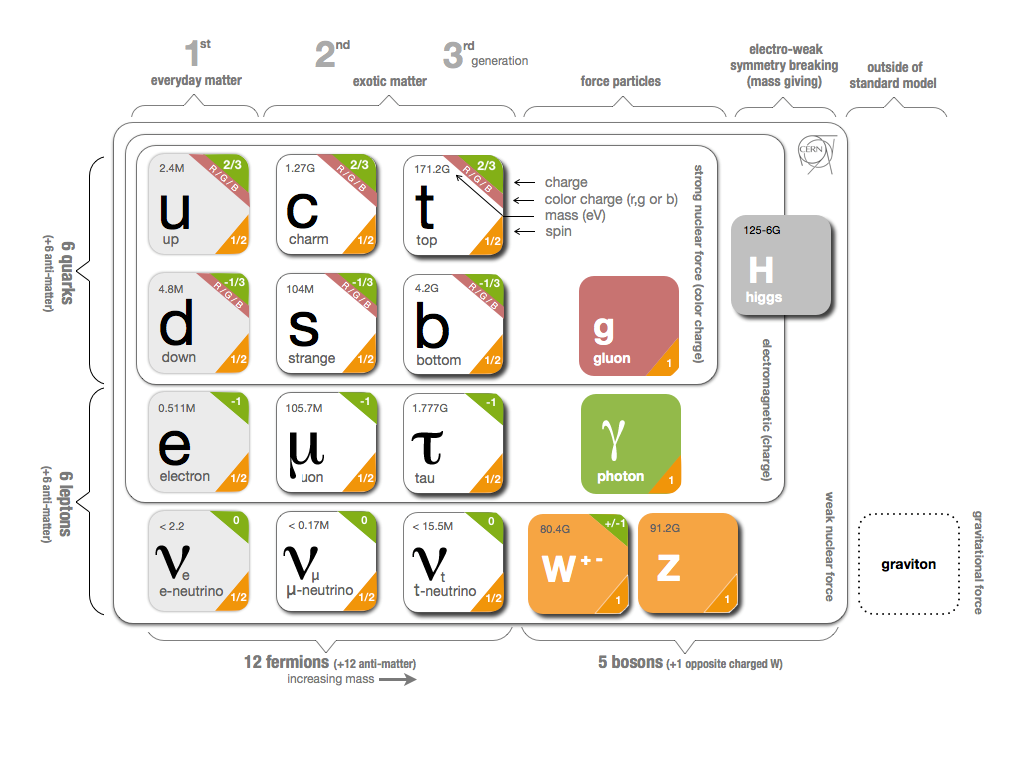
\includegraphics[width=\linewidth]{figures/theory/standard_model.png}
    \caption{ Table of all observed fundamental particles of the Standard
Model. \cite{Purcell:1473657}}
    \label{fig:standard_model}
  \end{center}
\end{figure}

\subsection{Bosons} \label{sec:theory:bosons}

The spin-1 particles are known as the vector gauge bosons and are the force
carriers of the SM.  The most commonly known is the electromagnetic force's
uncharged and massless photon ($\gamma$) which interacts with all particles
charged under $U(1)_{\text{em}}$ and is often referred to as ``light."  The
weak nuclear force is involved in nuclear interactions such as beta decays and
is carried by 3 bosons, all of which have mass and couple to fermions.  The
$W^{\pm}$ bosons mediate the charged weak interaction and allow for flavor
changing currents, while the $Z$ boson mediates the neutral weak interaction.
Finally there are 8 massless gluons which mediate the strong force and only
interact with fermions that have a ``color" charge such as the quarks contained
inside the nucleons. The only spin-0 boson, the Higgs Boson ($H$) is the key to
generating mass terms in the SM Lagrangian for the massive gauge bosons and for
fermions.  This is done through the so-called Higgs mechanism
\cite{Thomson:2013zua} and is discussed in more detail in
\Cref{sec:theory:higgs}.

\subsection{Fermions} \label{sec:theory:fermions}

The spin-1/2 particles can be further broken up into two distinct families of
particles, the leptons and the quarks, both of which contain three
``generations" each with an ``up"- and ``down"-type particle where ``up" and
``down" differentiate the two components of the weak isospin doublet.  The
``down"-type leptons are the electrically charged electron ($e$), muon ($\mu$)
and tau ($\tau$) while the ``up"-type are their electrically neutral
counterparts $\nu_e$, $\nu_\mu$, $\nu_\tau$. The ``up"-type quarks are the up
($u$), charm ($c$), and top ($t$), each with a $+2/3$ electric charge, while
the ``down"-type quarks are the down ($d$), strange ($s$), and bottom ($b$),
all of which have a $-1/3$ electric charge.  Each quark carries a ``color"
charge thus allowing them to couple to gluons and  participate in strong force
interactions.  Due to the observed color confinement of the strong force these
quarks are only observed in colorless bound states known as ``mesons" (1 quark
and 1 anti-quark) and ``baryons" (3 quarks or anti-quarks).  All of the above
fermions have an anti-particle partner with the opposite weak isospin.

\section{Quantum Electrodynamics} \label{sec:theory:qed}

In the SM the Electromagnetic and Weak nuclear forces are unified into the
Electroweak interaction which is represented by the $SU(2)_L \times U(1)_Y$
gauge group. The L represents the physical observable that the Weak interaction,
and thus the $SU(2)$ transformation, only acts on left handed particle states.
The Y states that this is the $U(1)$ symmetry for the weak hypercharge Y instead
of the electromagnetic charge.  The particle states for these interactions are
solutions to the Dirac equation and are represented as Dirac spinor doublets
($\boldsymbol{\Psi_L}$) for the left handed states, and as Dirac spinor singlets
($\Psi_R$) for the right handed states.  Thus when a general transformation from
the Electroweak gague group is applied to the left handed spinor doublet you get
\Cref{eq:qed:doublet}

\begin{equation} \label{eq:qed:doublet} 
\boldsymbol{\Psi_L} \rightarrow \boldsymbol{\Psi_L}^{'} = exp \left(
\underbrace{ ig^{'} \frac{Y_L}{2}
\zeta (x) }_{U(1)_Y} + \underbrace{ ig_{W} \boldsymbol{\alpha}(x) \cdot
\text{\bf{T}} }_{SU(2)_L} \right) \boldsymbol{\Psi_L}.
\end{equation}

For the right handed spinor singlet the $SU(2)_L$ doesn't contribute and
you get \Cref{eq:qed:singlet}

\begin{equation} \label{eq:qed:singlet} 
{\Psi_R} \rightarrow \Psi_R^{'} = exp \left( \underbrace{ ig^{'} \frac{Y_R}{2}
\zeta (x) }_{U(1)_Y} \right) \Psi_R.
\end{equation}

We can see that these local gauge transformations have introduced space-time
dependant terms $\boldsymbol{\alpha}(x)$ and $\zeta(x)$ into our electroweak
Lagrangian.  Due to the derivatives contained within the kinetic term of this
lagrangian, this new configuration would introduce additional terms, thus
violating our required local gauge invariance.  Luckily, we can remove these
additional terms by replacing the standard derivative ($\partial_{\mu}$) with th
covariant derivative ($D_{\mu}$) as seen in \Cref{eq:qed:left} for the
left handed states and \Cref{eq:qed:right} for the right handed states.

\begin{align} 
\label{eq:qed:left} 
D_\mu &= \partial_{\mu}
- \underbrace{\frac{1}{2}ig^{'}B_{\mu}Y_{L}}_{U(1)_Y} -
  \underbrace{\frac{1}{2}ig_{W}\bf{W}_\mu \cdot \boldsymbol{\tau}}_{SU(2)_L} \\
\label{eq:qed:right} 
D_\mu &= \partial_{\mu}  - \underbrace{\frac{1}{2}ig^{'}B_{\mu}Y_{R}}_{U(1)_Y} 
\end{align}

Here we see two new gauge fields; $B_\mu$ the weak hypercharge field and
$\boldsymbol{W_\mu}$ the charged weak field as well as the associated coupling
constants $g^{'}, g_{W}, Y_{L}, Y_{R}$ and the $SU(2)$ generators
$\boldsymbol{\tau}$.   Next we right down the transformation properies of these
new fields 

\begin{align}
\boldsymbol{W}_{\mu}(x) &\rightarrow \boldsymbol{W}_{\mu}^{'}(x) =
\boldsymbol{W}_{\mu} + \partial_{\mu} \boldsymbol{\alpha}(x) +
g_{W}\boldsymbol{W}_{\mu}(x) \times \boldsymbol{\alpha}(x)
\\ 
B_{\mu} &\rightarrow B_{\mu}^{'} = B_{\mu} +
\frac{1}{g^{'}}\partial_{\mu}\zeta(x)
\end{align}

The form of these fields is chosen such that the final Lagrangian is invariant
under $SU(2)_L \times U(1)_Y$ transformations, and thus we have restored gauge
invariance for the kinetic term of our electroweak Lagrangian!  Inserting these
new definitions into the Lagrangian for the spinor field $\Psi$ which satisfies
the free-particle Dirac equation we get

\begin{equation} \label{eq:qed:fermion_lagrangian}
\mathcal{L} = i\boldsymbol{\bar{\Psi}_L}\gamma^{\mu} \left( \partial_{\mu}
- \frac{1}{2}ig^{'}B_{\mu}Y_{L} - \frac{1}{2}ig_{W}\bf{W}_\mu \cdot
  \boldsymbol{\tau} \right) \boldsymbol{\Psi_L} + i \bar{\Phi}_{R}\gamma^{\mu}
\left(\partial_{\mu} - \frac{1}{2}ig^{'}B_{\mu}Y_{R} \right) \Phi_{R}
\end{equation}

Next we must construct the gauge field self interaction and mass terms

\begin{equation} \label{eq:qed:gauge_lagrangian}
\mathcal{L} = -\frac{1}{4}\boldsymbol{F}_{\mu\nu}\boldsymbol{F}^{\mu\nu}
-\frac{1}{4}B_{\mu\nu}B^{\mu\nu} +
\frac{1}{2}M_{W}^{2}\boldsymbol{W}_{\mu}\boldsymbol{W}^{\mu} +
\frac{1}{2}M_{B}^{2}B_{\mu}B^{\mu}
\end{equation}

where the field tensors $\boldsymbol{F}^{\mu\nu}$ and $B^{\mu\nu}$ are defined
to be

\begin{align}
\boldsymbol{F}^{\mu\nu}  &= \partial^{\mu}\boldsymbol{W}^{\nu} -
\partial^{\nu}\boldsymbol{W}^{\mu} + g\boldsymbol{W}^{\mu} \times
\boldsymbol{W}^{\nu} \\
B^{\mu\nu} &=  \partial^{\mu}\boldsymbol{B}^{\nu} -
\partial^{\nu}\boldsymbol{B}^{\mu}
\end{align}

The field tensor terms in \Cref{eq:qed:gauge_lagrangian} are invariant
under our gauge transformations, but simply plugging in
\Cref{eq:qed:left} or \Cref{eq:qed:right} into the mass terms shows that
these terms violate gauge invariance thus implying $M_{W} = 0$ and $M_{B} = 0$
in direct contradiction of the observed masses of the weak gauge bosons.  This
issue arises again for fermion mass terms as illustrated below for the elctron
field ($e$) expanded in its chiral basis.

\begin{equation}
m_{e}\bar{e}e = m_{e} \left( \begin{matrix}e^{\dagger}_{R} &
e^{\dagger}_{L} \end{matrix} \right) \left( \begin{matrix} e_{L}
\\ e_{R} \end{matrix} \right) = m_{e}(e^{\dagger}_{R}e_{L} +
e^{\dagger}_{L}e_{R})
\end{equation}

Remembering that the left and right handed spinors of the electroweak
interaction transform differently we see that this mixture of right and left
fields violates gauge invariance. This again forces us to conclude that $m_{e} = 0$
in contradiction to the observation that the electron does indeed have mass. As
mentioned in \Cref{sec:theory:bosons} the resolution to these mass
mysteries lies in the Higgs mechanism discussed in
\Cref{sec:theory:higgs}


Quantum Chromodynamics is the continuation of the mathematical framework
established by the electroweak formalism in (\Cref{sec:theory:gsw}, this time
for the strong force described by the $SU(3)_C$ gauge group, where $C$
represents the ``color" charge of QCD \cite{Campbell:2017hsr}.  This
color charge doesn't imply actual visible color, but is useful as an analogy to
the visible spectrum where a combination of red, green, and blue generates
white.  For QCD the combination of red, green, and blue color charges can
result in a colorless object.  As mentioned in \Cref{sec:theory:fermions}, the
quarks have a color (anti-color) charge defining color triplet field which
transforms under the general $SU(3)$ transformation as

\begin{equation}
q = \left( \begin{matrix} q_{r} \\ q_{g} \\ q_{b} \end{matrix} \right)
\rightarrow q^{'} = exp \left( ig_{s} \sum_{k=1}^{8} \eta_{k}(x)
\frac{\lambda_k}{2} \right) q
\end{equation}

Here the $\lambda_{k}$ are the Gell-Mann generators for $SU(3)$, $\eta(x)_{k}$ is the
space-time dependency for each generator, and  $g_s$ is the strong coupling constant.
As with the electroweak Lagrangian, the introduction of these space-time dependent terms adds new
terms into the kinematic portion of the Lagrangian and spoils the gauge 
invariance.  Again, a covariant derivative is introduced 

\begin{equation}
D_{\mu} = \partial_{\mu} - ig_{s}G_{\mu}^{k}\frac{\lambda_{k}}{2}
\end{equation}

to restore gauge invariance. The $G_{\mu}^{k}$ are the new fields introduced
for the 8 gluons.  These new fields transform under $SU(3)$ as

\begin{equation} \label{eq:qcd:gluon_field}
G_{\mu}^{k} \rightarrow G_{\mu}^{'k} = G_{\mu}^{k} + \partial_{\mu}\eta_{k}(x) +
g_{s}f_{klm}\eta_{l}(x)G_{\mu}^{m}
\end{equation}

Given these definitions the QCD Lagrangian ($\mathcal{L}_{QCD}$) can be
constructed as 

\begin{equation} \label{eq:qcd:qcd_lagrangian}
\mathcal{L}_{QCD} = \bar{q}(i\gamma_{\mu}D^{\mu} - m_{q})q -
\frac{1}{4}G_{k}^{\mu\nu}G_{k\mu\nu}
\end{equation}

where the gluon field tensor $G_{k}^{\mu\nu}$ is defined as

\begin{equation} \label{eq:qcd:gluon_tensor}
G_{k}^{\mu\nu} = \partial^{\mu}G_{k}^{\nu} - \partial^{\nu}G_{k}^{\mu} +
g_{s}f_{klm}G_{\l}^{\mu}G_{m}^{\nu}.
\end{equation}

The strong force is peculiar in that experiments observe only colorless objects
in the form of bound states of quarks known as hadrons.  Qualitatively, the
potential between a bound state of quarks (meson or baryon) gets stronger with
separation, unlike the other forces.  At the point where the system would
separate into color-charged objects, it becomes energetically favorable to
produce a quark/anti-quark pair in a process known as hadronization.  In other
words, attempting to separate a bound quark state into its colored constituents
simply results in new colorless bound states.  This requirement of colorless
objects by the strong force is known as color confinement. For highly energetic
strong interactions at hadron colliders the result is an expanding chain of
hadronizing quarks and gluons and their decay products known as a jet.


\section{The Higgs Mechanism} \label{sec:theory:higgs}

The Higgs mechanism is the system by which the gauge bosons and fermions gain
mass through the spontaneous breaking of the electroweak symmetry of the Higgs
potential \cite{Higgs:1964ia,Higgs:1966ev,Thomson:2013zua}.  This section will
also discuss briefly the couplings of the Higgs boson to massive particles, as
well as its self couplings.

\subsection{Electroweak Symmetry Breaking}

The Higgs field is expressed as a complex doublet, $\boldsymbol{\Phi}$, and thus
has four components defined as

\begin{equation} \label{eq:higgs:higgs_field}
\boldsymbol{\Phi}(x) = \left( \begin{matrix} \phi^{+} \\ \phi^{0} \end{matrix}
\right) = \frac{1}{\sqrt{2}} \left( \begin{matrix} \phi_{1}(x) + i\phi_{2}(x) \\
\phi_{3}(x) + i\phi_{4}(x) \end{matrix} \right).
\end{equation}

The four components of this field each represent a degree of freedom which
become the longitudinal polarizations of the $W^{\pm},Z$ gauge bosons and the
Higgs boson.  The resulting Lagrangian for the Higgs includes a kinetic term
(K) as well as the Higgs potential (V), all of which are invariant under the
electroweak gauge symmetry $SU(2)_L \times U(1)_Y$.  The definition is

\begin{equation} \label{eq:higgs:lagrangian}
\mathcal{L}_{\text{Higgs}} =
\underbrace{(D_{\mu}\boldsymbol{\Phi)^{\dagger}}D^{\mu}\boldsymbol{\Phi}}_{\text{K}}
- (\underbrace{\mu^{2}\boldsymbol{\Phi}^{\dagger}\boldsymbol{\Phi} +
  \lambda(\boldsymbol{\Phi}^{\dagger}\boldsymbol{\Phi})^{2}}_{\text{V}}).
\end{equation}

Here the $\mu^{2} < 0$ and $\lambda > 0$ are constrained such that the
potential forms a ring stable minima.  The shape of this potential is shown in
\Cref{fig:higgs_potential} and is often described as the ``Mexican-hat" or
"wine-bottle" potential. 

\begin{figure}[!h]
  \begin{center}
    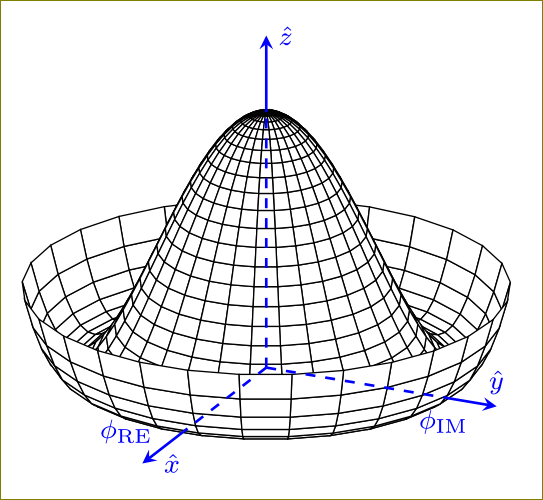
\includegraphics[width=0.4\linewidth]{figures/theory/higgs_potential.png}
    \caption{ A lower-dimensionality representation of the shape of the Higgs
potential.  The central peak represents a rotationally symmetric
unstable state, while the trough represents the infinite number of minima that
can be selected upon the spontaneous breaking of the symmetry.}
    \label{fig:higgs_potential}
  \end{center}
\end{figure}

The normed value of this minima can be calculated by taking the derivative of V
with respect to $\boldsymbol{\Phi}$ and setting it equal to $0$. This value,
also known as the vacuum expectation value (vev) has been found to be $v \equiv
\sqrt{-\mu^{2}/\lambda} = 246$ GeV. The arbitrary vev of the ground state Higgs
field is acquired when the symmetry of the Higgs potential is spontaneously
broken.  For ease of calculation the coordinate system is oriented such that

\begin{equation}
\left\langle \boldsymbol{\Phi}(x) \right\rangle = \frac{1}{\sqrt{2}} \left(
\begin{matrix} 0 \\ v \end{matrix} \right)
\end{equation} 

Next small perturbations around the minimum of the Higgs
potential are parametrized as 

\begin{equation} \label{eq:higgs:broken_higgs}
\left\langle \boldsymbol{\Phi}(x) \right\rangle = \frac{1}{\sqrt{2}} \left(
\begin{matrix} 0 \\ v + h(x) \end{matrix} \right) \text{exp} \left(
i\frac{\tau^{i}}{2}\theta^{i}(x) \right)
\end{equation} 

Here the real scalar field $h(x)$ corresponds to radial perturbations of the
minima, and the three $\theta^{i}(x)$ are the Nambu-Goldstone fields with
values determined by the choice of gauge.  Choosing the unitary gauge of
$\theta^{i}(x) = 0$ and expanding the kinetic term of
\Cref{eq:higgs:lagrangian} around the vev gives

\begin{equation} \label{eq:higgs:boson_masses}
\mathcal{L}_{\text{Higgs},K} = \frac{g^{2}v^{2}}{8} \left(
(W_{\mu}^{-})^{\dagger}W^{-\mu} + (W_{\mu}^{+})^{\dagger}W^{+\mu} \right) +
\frac{1}{2} \left( \begin{matrix} W_{\mu}^{3\dagger} & B_{\mu}^{\dagger}
\end{matrix} \right) \boldsymbol{M}^{2} \left( \begin{matrix} W^{3\mu} \\ B^{\mu}
\end{matrix} \right) + \ldots 
\end{equation}

Here the first term is the physical mass term for the $W^{\pm}$ bosons where
these charge eigenstates have been constructed out of the $W^{1,2}$ fields as
such $W^{\pm} = \frac{1}{\sqrt{2}}(W^{1} \mp iW^{2})$.  The second term
represents the mixture of the $W^{3}$ and $B$ fields through the mass matrix
$\boldsymbol{M}$.  Diagonalizing this matrix ($M_{D}$) and identifying the mass
eigenstates gives the physical fields of the photon ($\gamma$) and the $Z$
boson

\begin{equation}
\boldsymbol{M}_{D}^{2} = \left( \begin{matrix} 0 & 0 \\ 0 &
\frac{v^{2}}{4}(g_{W}^{2} + g^{'2)}   \end{matrix} \right)
\end{equation}

The upper left diagonal element corresponds to the massless photon
while the lower right diagonal element gives the mass of the massive $Z$ boson.
This results in the following masses for the four electroweak bosons

\begin{equation}
m_{W} = \frac{1}{2}g_{W}v \quad , \quad m_Z = \frac{1}{2}v\sqrt{g_{W}^{2} + g^{'2}}
\quad , \quad m_\gamma = 0
\end{equation}

The masses of the $W^{\pm}$ and $Z$ gauge bosons can be related through the
Weinberg mixing angle defined as

\begin{equation}
\theta_W = \cos^{-1}\left( \frac{g_{W}}{\sqrt{g_{W}^{2}+g^{'2}}} \right) \rightarrow m_{Z} =
\frac{m_{W}}{\cos{\theta_{W}}}
\end{equation}

Using this definition one can write out the exact mixture of $B$ and $W^{3}$ that
make up the photon and $Z$ boson as

\begin{align}
\gamma &= \text{cos}(\theta_{W})B + \text{sin}(\theta_{W})W^{3} \\
Z &= -\text{sin}(\theta_{W})B + \text{cos}(\theta_{W})W^{3}
\end{align}

\subsection{Fermion Mass Terms} \label{sec:theory:fermion_mass}

\Cref{sec:theory:gsw} shows how a simple fermion mass terms violate gauge
invariance due to the mixing of the left and right chiral states.  The Higgs
mechanism, however, allows for a gauge-invariant method of generating mass
terms through the Yukawa coupling of the Higgs field to the fermion fields.  An
example is the Yukawa coupling term for a quark doublet
($\boldsymbol{\Psi}_{L}$) and singlet ($\Psi_R$) coupling to the Higgs field
($\boldsymbol{\Phi}$) after spontaneous symmetry breaking, with the form
shown in \Cref{eq:higgs:broken_higgs}, when the unitary gauge $\Phi^{i}(x) = 0$
is chosen.
%
\begin{align}
\mathcal{L}_{\text{Yukawa}} &= - g_{b} \left[ \boldsymbol{\bar{\Psi}_L}
\boldsymbol{\Phi} \Psi_R + \bar{\Psi}_{R} \boldsymbol{\Phi}^{\dagger} \boldsymbol{\Psi_L}
\right] \\ &= - \frac{g_{b}}{\sqrt{2}} \left[ \left( \begin{matrix}
\bar{t} & \bar{b} \end{matrix} \right)_L \left( \begin{matrix} 0 \\ v +
h \end{matrix} \right) b_{R} + \bar{b}_{R} \left( \begin{matrix} 0 & (v + h)
\end{matrix} \right) \left( \begin{matrix} t \\ b \end{matrix} \right)_L \ \right] \\ &= - \underbrace{\frac{g_{b}}{\sqrt{2}}
v}_{m_{b}} \left( \bar{b}_{L}b_{R} + \bar{b}_{R}b_{L}  \right)
- \underbrace{\frac{g_{b}}{\sqrt{2}}}_{g_{b,h}} h \left(
\bar{b}_{L}b_{R} + \bar{b}_{R}b_{L}  \right) 
\end{align}
%
In this way mass terms are generated for the fermion field and the gauge
invariance of the Lagrangian is maintained via the proper combination of
covariant derivatives and fields.  This operation also produces the second term
which represents the coupling of the bottom quark to the Higgs itself and thus
gives the form of its coupling constant $g_{b,h}$.  Using this newly found
mass of the bottom quark $m_{b}$ the coupling can be written as
%
\begin{equation}
g_{b,h} = \frac{g_{b}}{\sqrt{2}} = \frac{m_{b}}{v}.
\end{equation}
%
Thus the coupling of the Higgs boson to a fermion is proportional
to the mass of the fermion itself. 
 
\subsection{The Higgs Boson}

It has been shown that the Higgs mechanism properly mixes the gauge fields to
provide the correct gauge-invariant mass terms, and also properly combines the
left and right chiral states of fermions to produce their mass terms.  During
spontaneous symmetry breaking of the electroweak potential three of the four
degrees of freedom in the Higgs doublet (\Cref{eq:higgs:higgs_field}) become
Goldstone bosons.  Since this theory is gauged these Goldstone bosons are
``eaten" by the 3 gauge bosons $W^{\pm}$ and $Z$ to form their longitudinal
components thus give them their mass.  However, the final broken degree of
freedom is absorbed by the new massive scalar particle, the Higgs boson
\cite{Higgs:1964pj}.

Focusing on the Higgs potential term (V) of
\Cref{eq:higgs:lagrangian} and substituting in the definition for
$\boldsymbol{\Phi}$ given in \Cref{eq:higgs:broken_higgs} gives
%
\begin{equation}
\mathcal{L}_\text{Higgs,V} = \frac{1}{2} \mu^{2} v^{2} - \mu^{2} h^{2} +
\lambda v h^{3} + \frac{1}{4} \lambda h^{4}
\end{equation}
%
The first term is constant and thus can be ignored.  The second term is the
mass term for the Higgs boson, $m_h = \sqrt{-2\mu^{2}} = \sqrt{2\lambda}v$.
Remembering that $h = h(x)$ was used for small radial perturbations of the
Higgs field the Higgs boson can be identified as a radial excitation of the
Higgs field.  Finally, the third and fourth terms represent the Higgs boson
self-couplings.  With these couplings and mass terms in hand the next step is
to experimentally verify this theory as discussed next in \Cref{chap:higgs}.



\chapter{Boosted Higgs at the LHC} \label{chap:higgs}

The Higgs mechanism, as described in \Cref{sec/theory/gsw} solves the
problem of generating gauge boson and fermion mass terms while also maintaining
gauge invariance.  To understand the search for the SM Higgs boson requires the
discussion of how one goes about producing and detecting it.  In order to
gather sufficient data to validate the theory a collider capable of
putting enough energy into a collision to rapidly produce Higgs bosons for
study is required.  To this end the Large Hadron Collider (LHC) discussed in
\Cref{chap:lhc} was laboriously designed, funded, and constructed by the
largest international collaboration of collider physicists and engineers on the
planet. This chapter will include a discussion of the relevant Higgs boson
production mechanisms available at the LHC and the various decay modes of the
Higgs boson that are used to measure its properties including the final state
that is the focus of this dissertation.

\section{Higgs Production Mechanisms} \label{sec:higgs:production}

At the LHC the dominant production mechanisms for the Higgs boson in order of
decreasing cross section are: gluon-fluon fusion (ggF), vector boson fusion
(VBF), vector boson associated production or ``Higgsstrahlung" (VH), and
associated production with $t\bar{t}$ ($t\bar{t}H$) and $b\bar{b}$
($b\bar{b}H$).  The cross sections for the signatures of these processes with
associated theoretical uncertainties for each are shown as a function of the
center-of-mass energy $\sqrt{s}$ in \Cref{fig:higgs_xsection}, and the
leading order (LO) Feynman diagrams can be seen in \Cref{fig:higgs_production}.

\begin{figure}[!htbp]
  \begin{center}
    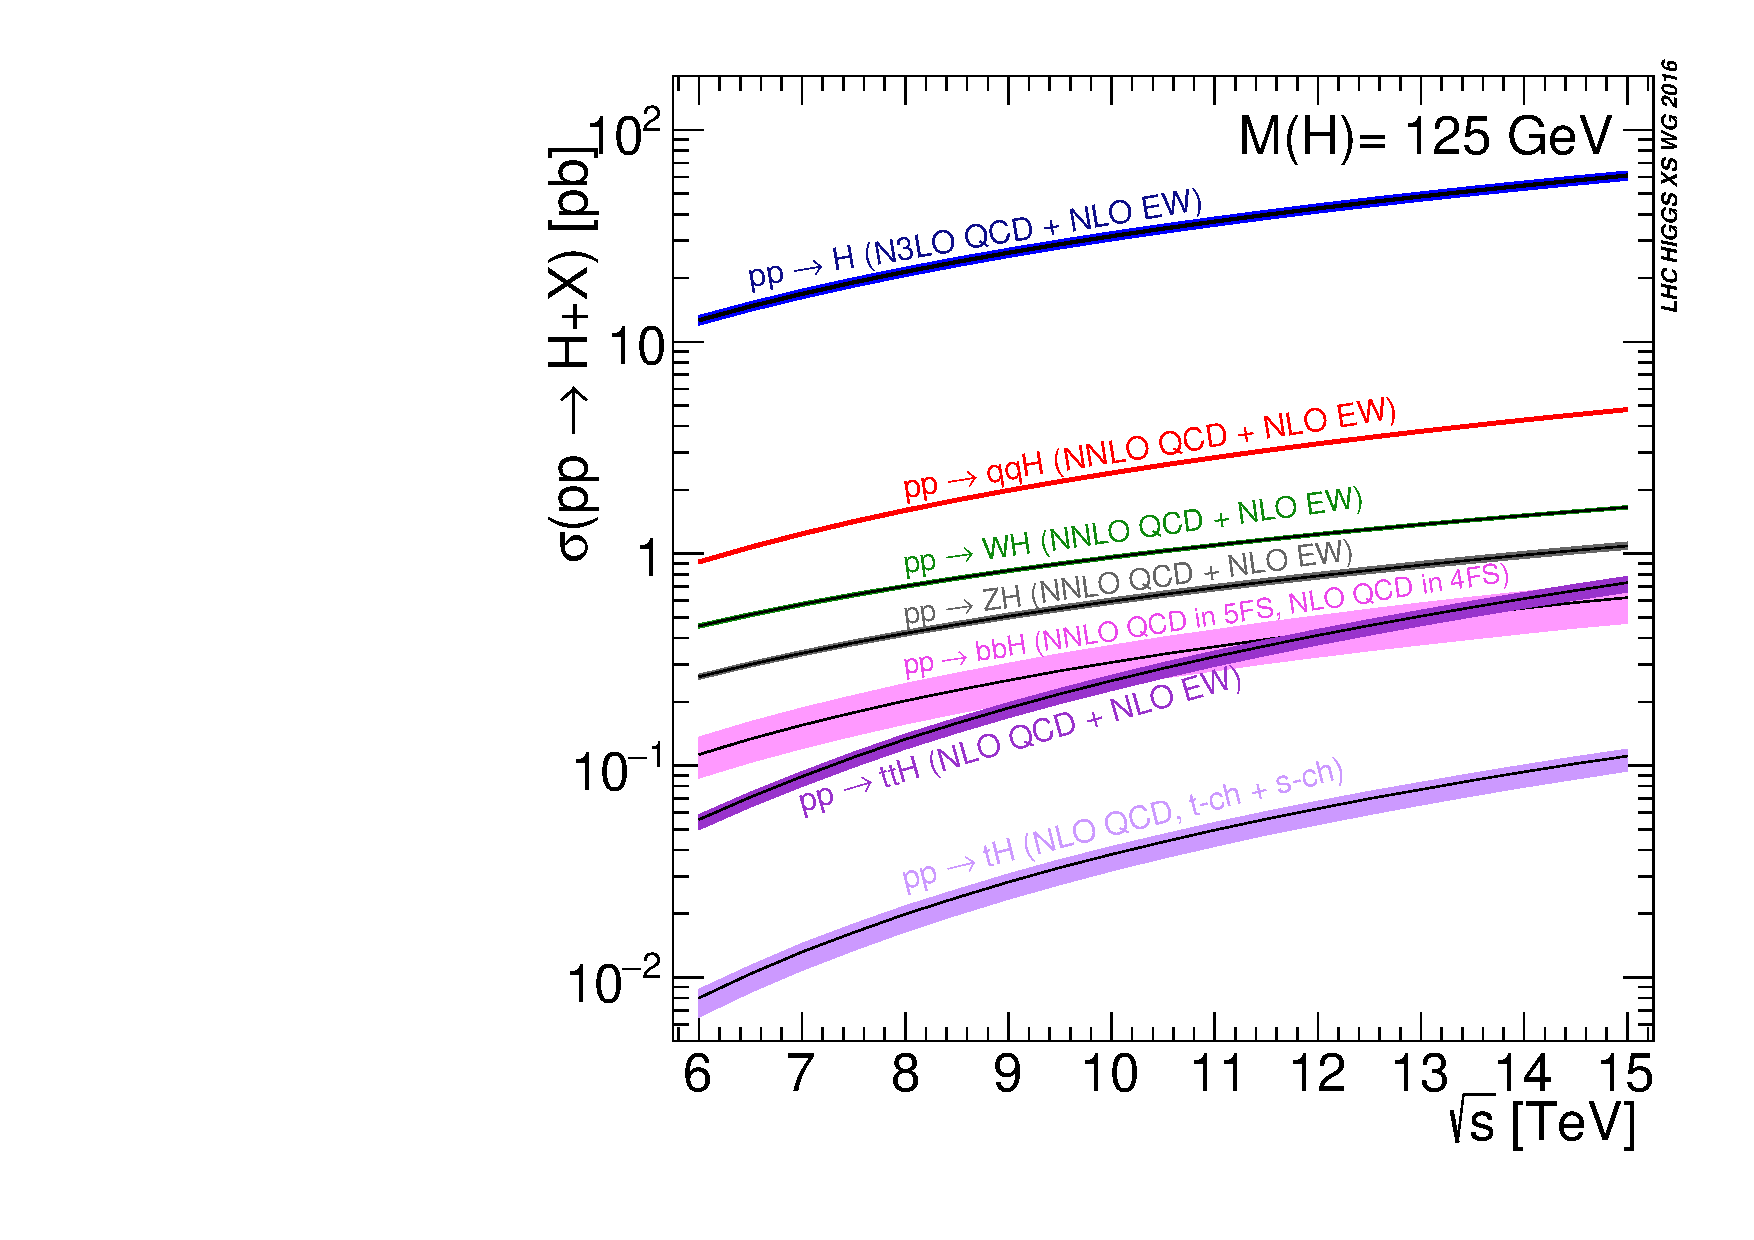
\includegraphics[width=0.5\linewidth]{figures/higgs/higgs_xsection.pdf}
    \caption{Cross sections for the production of the SM Higgs boson signatures
as a function of the center of mass energy ($\sqrt{s}$) at the LHC
\cite{PDG2018:Ch11}.  In order of decreasing cross section: the ggF process
signature is $H$, the VBF process signature is $qqH$, the VH process signature
is split into $WH$ and $ZH$, and the $b\bar{b}$ / $t\bar{t}$ signatures are
$t\bar{t}H$ / $b\bar{b}H$.}
    \label{fig:higgs_xsection}
  \end{center}
\end{figure}

The LO Feynman diagram contains the least number of vertices, and thus coupling
constants, making it the largest contribution to the cross section calculation.
Adding an additional vertex, represents a higher order correction to the LO
calculation known as next-to-leading order (NLO) where each additional vertex
adds a ``next" (NNLO, N3LO, etc.). For reference, the current best
estimates of the production cross sections for the leading production
mechanisms are detailed in \Cref{table:higgs_production_xsection}.

\begin{figure}[!htbp]
\centering

\subcaptionbox{gluon-gluon fusion}{
\resizebox{0.48\textwidth}{!}{
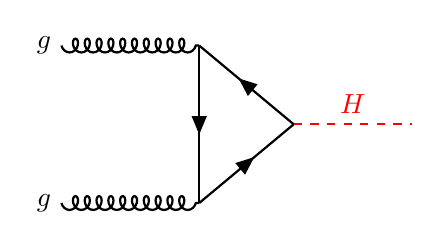
\begin{tikzpicture}[thick]
 \begin{feynman}
  \vertex (origin);
  \vertex [right=1.5cm of origin] (H);
  \vertex [above left=1cm and 1.2cm of origin] (v1);
  \vertex [below left=1cm and 1.2cm of origin] (v2);
  \vertex [left=1.75cm of v1] (g1) {\(g\)};
  \vertex [left=1.75cm of v2] (g2) {\(g\)};
  \diagram* {
  (origin) -- [red, scalar, edge label={\(H\)}] (H),
  (origin) -- [fermion] (v1) -- [fermion] (v2) -- [fermion] (origin),
  (g1) -- [gluon] (v1),
  (g2) -- [gluon] (v2),
  };
 \end{feynman}
\end{tikzpicture}
}}
\subcaptionbox{vector boson fusion}{
\resizebox{0.48\textwidth}{!}{
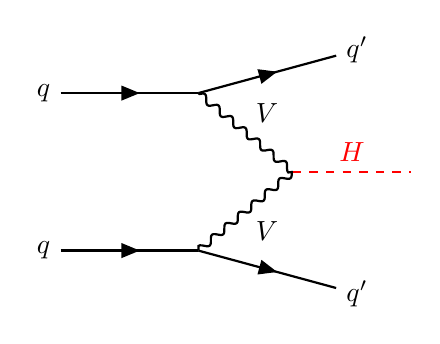
\begin{tikzpicture}[thick]
 \begin{feynman}
  \vertex (origin);
  \vertex [right=1.5cm of origin] (H);
  \vertex [above left=1cm and 1.2cm of origin] (v1);
  \vertex [below left=1cm and 1.2cm of origin] (v2);
  \vertex [left=1.75cm of v1] (q1) {\(q\)};
  \vertex [left=1.75cm of v2] (q2) {\(q\)};
  \vertex [above right=0.25cm and 1.75cm of v1] (q3) {\(q'\)};
  \vertex [below right=0.25cm and 1.75cm of v2] (q4) {\(q'\)};
  \diagram* {
  (v1) -- [boson, edge label={\(V\)}] (origin),
  (origin) -- [boson, edge label={\(V\)}] (v2),
  (origin) -- [red, scalar, edge label={\(H\)}] (H),
  (q1) -- [fermion] (v1),
  (q2) -- [fermion] (v2),
  (v1) -- [fermion] (q3),
  (v2) -- [fermion] (q4),
  };
 \end{feynman}
\end{tikzpicture}
}} \\
\subcaptionbox{associated production}{
\resizebox{0.48\textwidth}{!}{
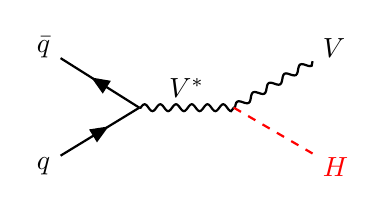
\begin{tikzpicture}[thick]
 \begin{feynman}
  \vertex (origin);
  \vertex [right=1.2cm of origin] (Vstar);
  \vertex [above right=0.50cm and 1.0cm of Vstar] (V1) {\(V\)};
  \vertex [red, below right=0.50cm and 1.0cm of Vstar] (H) {\(H\)};
  \vertex [above left=0.50cm and 1.0cm of origin] (g1) {\(\bar{q}\)};
  \vertex [below left=0.50cm and 1.0cm of origin] (g2) {\(q\)};
  \diagram* {
  (origin) -- [boson, edge label={\(V^{*}\)}] (Vstar) -- [boson] (V1),
  (Vstar) -- [red, scalar] (H),
  (origin) -- [fermion] (g1),
  (g2) -- [fermion] (origin),
  };
 \end{feynman}
\end{tikzpicture}
}}
\subcaptionbox{$t\bar{t}$ ($t\bar{t}H$) and $b\bar{b}$ ($b\bar{b}H$)}{
\resizebox{0.48\textwidth}{!}{
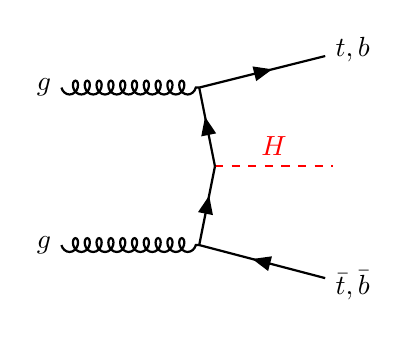
\begin{tikzpicture}[thick]
 \begin{feynman}
  \vertex (origin);
  \vertex [right=1.5cm of origin] (H);
  \vertex [above left=1cm and 0.2cm of origin] (v1);
  \vertex [below left=1cm and 0.2cm of origin] (v2);
  \vertex [left=1.75cm of v1] (g1) {\(g\)};
  \vertex [left=1.75cm of v2] (g2) {\(g\)};
  \vertex [above right=1.2cm and 1.4cm of origin] (t1) {\(t,b\)};
  \vertex [below right=1.2cm and 1.4cm of origin] (t2) {\(\bar{t},\bar{b}\)};
  \diagram* {
  (g1) -- [gluon] (v1),
  (g2) -- [gluon] (v2),
  (origin) -- [red, scalar, edge label={\(H\)}] (H),
  (origin) -- [fermion] (v1) -- [fermion] (t1),
  (t2) -- [fermion] (v2) -- [fermion] (origin),
  };
 \end{feynman}
\end{tikzpicture}
}}

\caption{Feynman diagrams representing the dominant Higgs production modes at
the LHC.}

\label{fig:higgs_production}
\end{figure}

\begin{table}[htpb]
 \centering
 \caption{ SM Higgs boson production cross sections in units of pb for
$m_{H}=125~\GeV$ in $pp$ collisions for the current LHC center-of-mass energy,
$\sqrt{s} = 13~\TeV$.  The predictions for the ggF channel include the latest
N3LO results, which have reduced theoretical uncertainties by a factor around 2
compared to the NNLO results \cite{PDG2018:Ch11}.}
 \begin{tabular}{@{}rrrrrrrr@{}} \toprule
  $\sqrt{s}~(\TeV)$ & ggF                  & VBF                  & $WH$                 & $ZH$                 & $t\bar{t}H$            & Total~(pb) \\ \midrule
  $13$              & $48.6_{-5\%}^{+5\%}$ & $3.78_{-2\%}^{+2\%}$ & $1.37_{-2\%}^{+2\%}$ & $0.88_{-5\%}^{+5\%}$ & $0.50_{-13\%}^{+9\%}$ &  $55.1$    \\
  \bottomrule
 \end{tabular}\label{table:higgs_production_xsection}
\end{table}

The dominant Higgs production mechanism at hadron colliders is gluon-gluon
fusion.  This may seem strange as gluons are massless and thus do not couple
directly to the Higgs boson.  Instead the gluons indirectly couple to the Higgs
boson via a quark loop.  As discussed in \Cref{sec:theory:fermion_mass}, the
coupling of a fermion is proportional to $m_f$, so the dominant contribution to
this quark loop comes from the top quark. It is important to note that the ggF
cross section in \Cref{table:higgs_production_xsection} is inclusive in number
of final state jets and thus will include diagrams like the one shown in
\Cref{fig:h_plus_j}.  There has been considerable effort to calculate exclusive
$H$ + jet(s) production process at NLO and NNLO \cite{deFlorian:2016spz} for
use in analysis where there is an explicit requirement for an associated jet
such as the one presented in this dissertation in \Cref{part:HbbISR}.

\begin{figure}[!htbp]
\centering
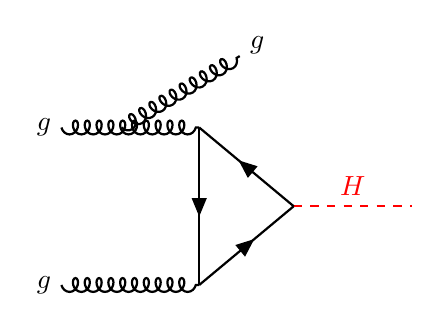
\begin{tikzpicture}[thick]
 \begin{feynman}
  \vertex (origin);
  \vertex [right=1.5cm of origin] (H);
  \vertex [above left=1cm and 1.2cm of origin] (v1);
  \vertex [below left=1cm and 1.2cm of origin] (v2);
  \vertex [left=1.75cm of v1] (g1) {\(g\)};
  \vertex [left=1.75cm of v2] (g2) {\(g\)};
  \vertex at ($(g1)!0.5!(v1)$) (ISR_start);
  \vertex [above right=0.8cm and 1.5 cm of ISR_start] (ISR) {\(g\)};
  \diagram* {
  (origin) -- [red, scalar, edge label={\(H\)}] (H),
  (origin) -- [fermion] (v1) -- [fermion] (v2) -- [fermion] (origin),
  (g1) -- [gluon] (v1),
  (g2) -- [gluon] (v2),
  (ISR_start) -- [gluon] (ISR),
  };
 \end{feynman}
\end{tikzpicture}
\caption{Feynman diagram for ggF Higgs + jet production.}
\label{fig:h_plus_j}
\end{figure}

The second-largest cross section for Higgs production at the LHC comes from the VBF
mechanism.  In VBF the initial state quarks scatter via the exchange of a
$W^{\pm}$ or $Z$ boson which subsequently radiates the Higgs boson.  Unlike ggF
this production mechanism scatters the initial state quarks which allows them to
be observed as part of the interaction.  The presence of these extra quarks
makes these interactions easier to select during analysis.

The third-largest cross section for Higgs production is in association with a
vector boson. The cross section for this is even smaller than the above two, but
remains important due to the easily selected signature of the decaying vector
boson.  The largest background at the LHC is multijet events coming from
interactions that produce strong force objects.  Thus the leptons from the
boson's decay act as a discriminator against this multijet background, greatly
reducing its effect on sensitivity. Note that the $W/Z$ can also decay
hadronically giving a final state that looks like $H$ + jet.

The lowest cross section of the four methods discussed is the
production of the Higgs boson in association with either $b\bar{b}$ or
$t\bar{t}$.  This channel is important because it allows direct measurement of
the $ttH$ coupling, unlike the ggF method where the quark in the loop is never
directly observed.

\section{Parton Distribution Function} \label{sec:higgs:partons}

The LHC collides protons, however looking at the feynman diagrams in
\Cref{fig:higgs_production} we see that it is quarks and gluons (a.k.a partons)
that produce these fundamental interactions. This is an indicator that when we
calculate the production cross section for a process at the LHC, we have to not
only consider the hard-scatter probability of the specific diagram, but also
consider the composition of the proton itself.  Specifically, we must consider
the fraction of the total momentum of the proton held by each of its constituent
partons.  This concept is described by Parton Distribution Functions (PDFs)
which give the probability that the indicated parton carries momentum fraction
$x$ of the proton when probed at with energy scale $Q$.  An example PDF for $Q =
10\text{GeV}^2$ and $Q = 10^{4}$GeV in \Cref{fig:parton_distribution_function}

\begin{figure}[!htbp]
  \begin{center}
    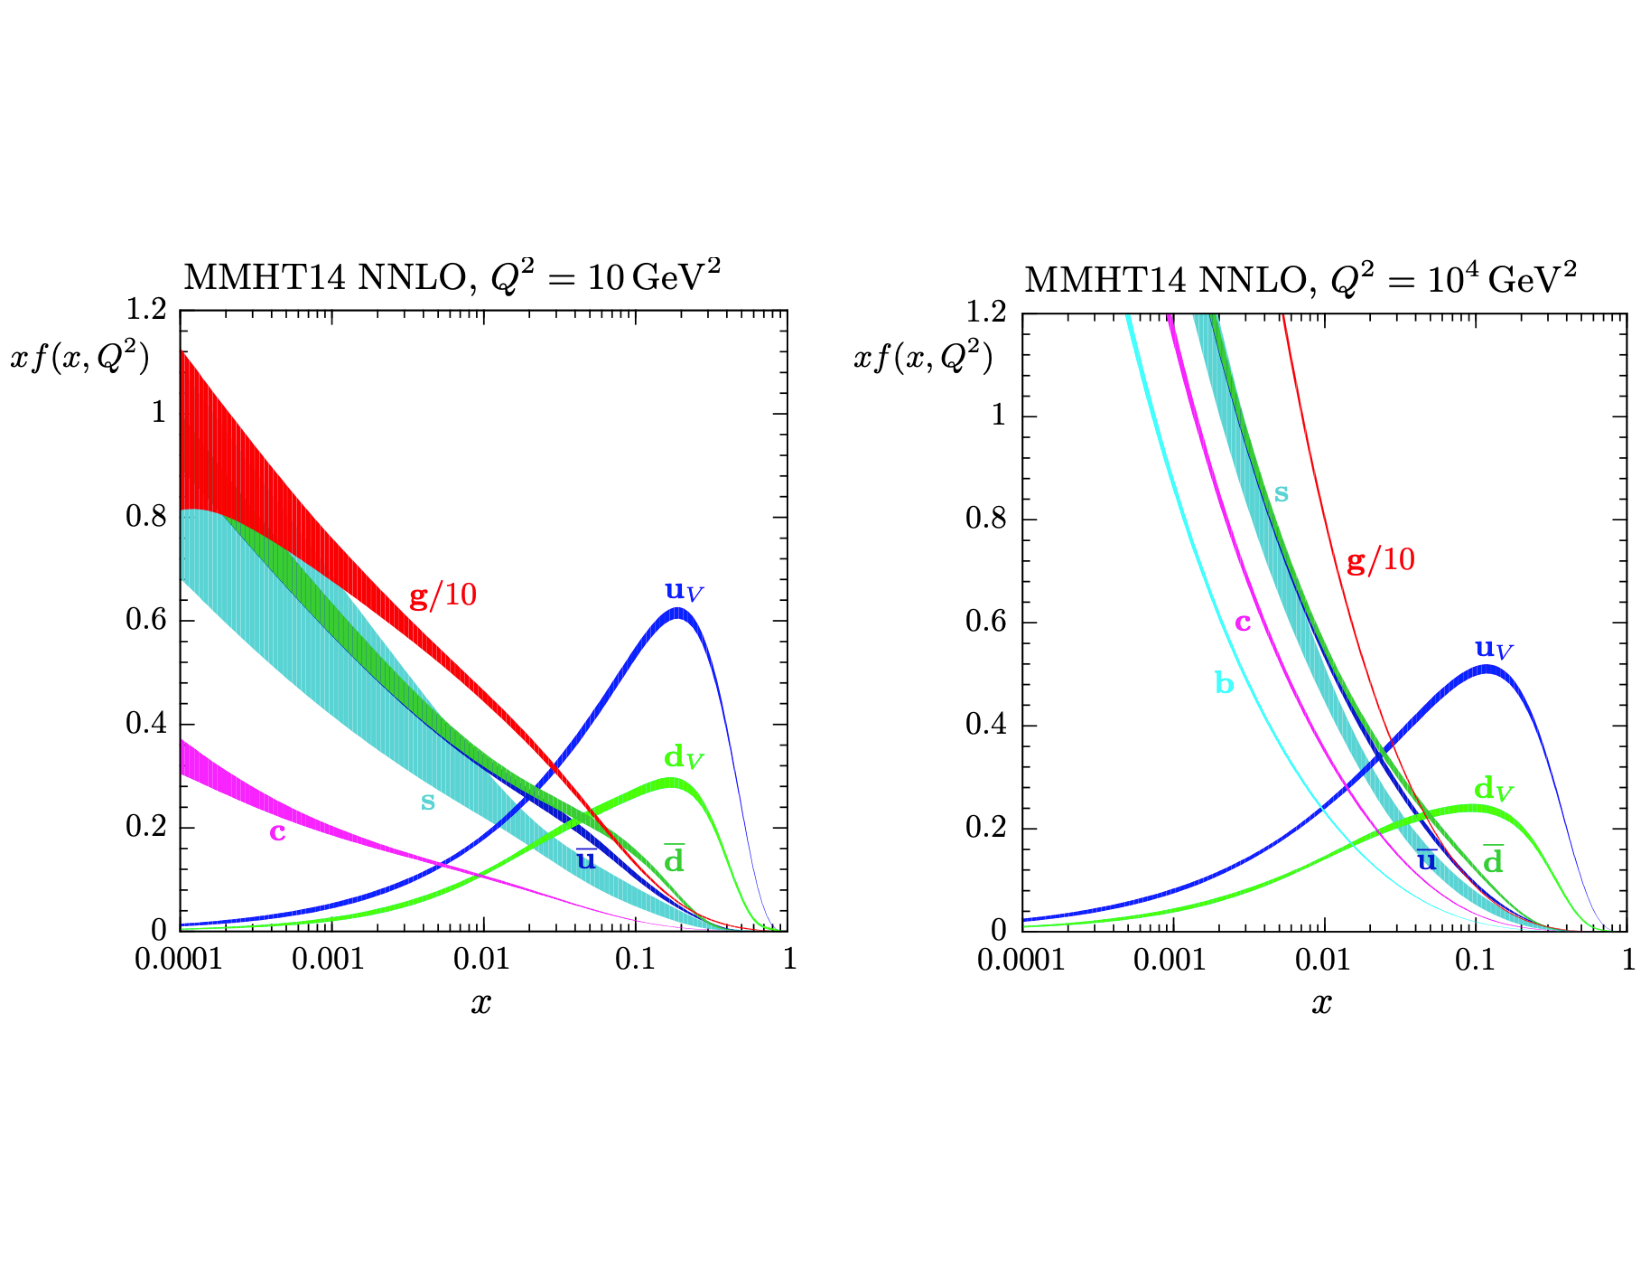
\includegraphics[width=0.8\linewidth]{figures/higgs/pdf.pdf}
    \caption{ \cite{Harland-Lang2015} MMHT2014 NNLO PDFs at $Q2 = 10\text{GeV}^{2}$ and $Q2
=10^{4}\text{GeV}^{2}$ with associated 68\% confidence-level uncertainty bands.
The colored regions indicate the probability of finding the labeled parton with
a momentum fraction given along the x axis. As expected the $u_V$ and $d_V$
contain the largest fraction of the momentum, however we can also see that many
gluons will exist with smaller fractions of the total momentum. Note that as
$Q^2$ increases you are more likely to find something besides a $u/d$}
    \label{fig:parton_distribution_function}
  \end{center}
\end{figure}

\section{Branching Ratios} \label{sec:higgs:branching}

The coupling of the SM Higgs with the gauge bosons and fermions has been shown
to give these particles their mass, however it also means that the Higgs can
decay into all of these particles.  In order of most to least likely final
states of a Higgs decay we have the decay to; a pair of $b$-quarks ($b\bar{b}$),
a pair of weak vector bosons where one is off-shell ($VV^{*}$), two gluons
($gg$), a duo of tau leptons ($\tau^{+}\tau^{-}$), or a pair of photons
($\gamma\gamma$).  Similar to the ggF production mechanism discussed in
\Cref{sec:higgs:production} the decays to massless gauge bosons (photons and
gluons) are facilitated through loops of massive particles. The exact feynman
diagrams depicting the above process' are shown in \Cref{fig:higgs_decay} while
information about their branching ratios is detailed in
\Cref{table:higgs_branching_ratios}.

\begin{figure}[!htbp]
\centering

\subcaptionbox{$H \rightarrow b\bar{b}$}{
\resizebox{0.48\textwidth}{!}{
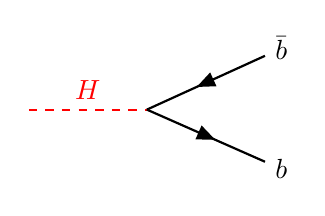
\begin{tikzpicture}[thick]
 \begin{feynman}
  \vertex (origin);
  \vertex [right=1.5cm of origin] (H);
  \vertex [above right=0.50cm and 1.5cm of H] (b1) {\(\bar{b}\)};
  \vertex [below right=0.50cm and 1.5cm of H] (b2) {\(b\)};
  \diagram* {
  (origin) -- [red, scalar, edge label={\(H\)}] (H),
  (b1) -- [fermion] (H) -- [fermion] (b2),
  };
 \end{feynman}
\end{tikzpicture}
}}
\subcaptionbox{$H \rightarrow W^{\pm}W^{\mp*}$}{
\resizebox{0.48\textwidth}{!}{
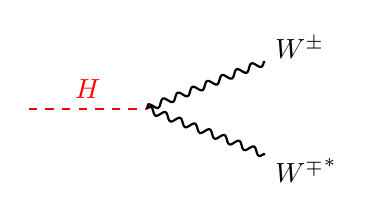
\begin{tikzpicture}[thick]
 \begin{feynman}
  \vertex (origin);
  \vertex [right=1.5cm of origin] (H);
  \vertex [above right=0.50cm and 1.5cm of H] (W1) {\(W^{\pm}\)};
  \vertex [below right=0.50cm and 1.5cm of H] (W2) {\({W^{\mp}}^{*}\)};
  \diagram* {
  (origin) -- [red, scalar, edge label={\(H\)}] (H),
  (W1) -- [boson] (H),
  (W2) -- [boson] (H),
  };
 \end{feynman}
\end{tikzpicture}
}} \\
\subcaptionbox{$H \rightarrow gg$}{
\resizebox{0.48\textwidth}{!}{
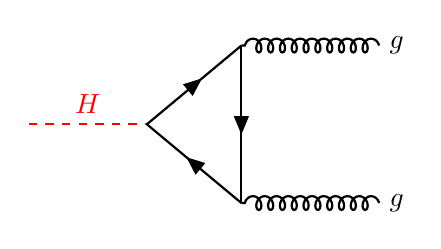
\begin{tikzpicture}[thick]
 \begin{feynman}
  \vertex (origin);
  \vertex [right=1.5cm of origin] (H);
  \vertex [above right=1cm and 1.2cm of H] (v1);
  \vertex [below right=1cm and 1.2cm of H] (v2);
  \vertex [right=1.75cm of v1] (g1) {\(g\)};
  \vertex [right=1.75cm of v2] (g2) {\(g\)};
  \diagram* {
  (origin) -- [red, scalar, edge label={\(H\)}] (H),
  (H) -- [fermion] (v1) -- [fermion] (v2) -- [fermion] (H),
  (g1) -- [gluon] (v1),
  (g2) -- [gluon] (v2),
  };
 \end{feynman}
\end{tikzpicture}
}}
\subcaptionbox{$H \rightarrow \tau^{+}\tau{-}$}{
\resizebox{0.48\textwidth}{!}{
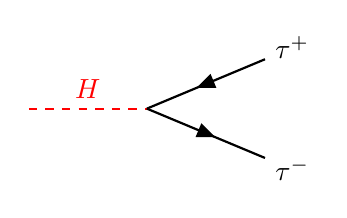
\begin{tikzpicture}[thick]
 \begin{feynman}
  \vertex (origin);
  \vertex [right=1.5cm of origin] (H);
  \vertex [above right=0.50cm and 1.5cm of H] (tau1) {\(\tau^{+}\)};
  \vertex [below right=0.50cm and 1.5cm of H] (tau2) {\(\tau^{-}\)};
  \diagram* {
  (origin) -- [red, scalar, edge label={\(H\)}] (H),
  (tau1) -- [fermion] (H) -- [fermion] (tau2),
  };
 \end{feynman}
\end{tikzpicture}
}} \\
\subcaptionbox{$H \rightarrow ZZ^{*}$}{
\resizebox{0.48\textwidth}{!}{
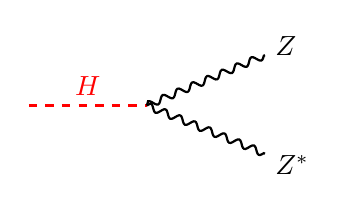
\begin{tikzpicture}[thick]
 \begin{feynman}
  \vertex (origin);
  \vertex [right=1.5cm of origin] (H);
  \vertex [above right=0.50cm and 1.5cm of H] (Z1) {\(Z\)};
  \vertex [below right=0.50cm and 1.5cm of H] (Z2) {\(Z^{*}\)};
  \diagram* {
  (origin) -- [red, scalar, edge label={\(H\)}] (H),
  (Z1) -- [boson] (H),
  (Z2) -- [boson] (H),
  };
 \end{feynman}
\end{tikzpicture}
}}
\subcaptionbox{$H \rightarrow \gamma\gamma$}{
\resizebox{0.48\textwidth}{!}{
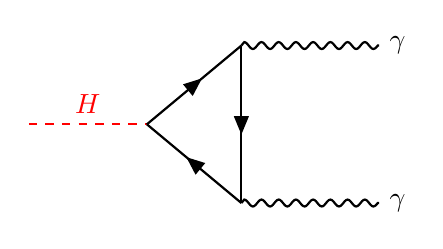
\begin{tikzpicture}[thick]
 \begin{feynman}
  \vertex (origin);
  \vertex [right=1.5cm of origin] (H);
  \vertex [above right=1cm and 1.2cm of H] (v1);
  \vertex [below right=1cm and 1.2cm of H] (v2);
  \vertex [right=1.75cm of v1] (gamma1) {\(\gamma\)};
  \vertex [right=1.75cm of v2] (gamma2) {\(\gamma\)};
  \diagram* {
  (origin) -- [red, scalar, edge label={\(H\)}] (H),
  (H) -- [fermion] (v1) -- [fermion] (v2) -- [fermion] (H),
  (gamma1) -- [photon] (v1),
  (gamma2) -- [photon] (v2),
  };
 \end{feynman}
\end{tikzpicture}
}}


\caption{Feynman diagrams representing the leading Higgs decay channels.}

\label{fig:higgs_decay}
\end{figure}

\begin{table}[htpb]
 \centering
 \caption{ The branching ratios and the relative uncertainty for a Standard Model Higgs boson with $m_{H}=125~\GeV$ \cite{PDG2018:Ch11}.}
 \begin{tabular}{@{}lrr@{}} \toprule
  Decay Channel           & Branching Ratio       & Relative Uncertainty \\ \midrule
  $H\to b\bar{b}$         & $5.84 \times 10^{-1}$ & $_{-3.3\%}^{+3.2\%}$ \\
  \addlinespace[0.3em]
  $H\to W^{+}W^{-}$       & $2.14 \times 10^{-1}$ & $_{-4.2\%}^{+4.3\%}$ \\
  \addlinespace[0.3em]
  $H\to \tau^{+}\tau^{-}$ & $6.27 \times 10^{-2}$ & $_{-5.7\%}^{+5.7\%}$ \\
  \addlinespace[0.3em]
  $H\to ZZ$               & $2.62 \times 10^{-2}$ & $_{-4.1\%}^{+4.3\%}$ \\
  \addlinespace[0.3em]
  $H\to \gamma\gamma$     & $2.27 \times 10^{-3}$ & $_{-4.9\%}^{+5.0\%}$ \\
  \addlinespace[0.3em]
  $H\to Z\gamma$          & $1.53 \times 10^{-3}$ & $_{-8.9\%}^{+9.0\%}$ \\
  \addlinespace[0.3em]
  $H\to \mu^{+}\mu^{-}$   & $2.18 \times 10^{-4}$ & $_{-5.9\%}^{+6.0\%}$ \\
  \bottomrule
 \end{tabular}\label{table:higgs_branching_ratios}
\end{table} 

In \Cref{table:higgs_branching_ratios} the order is determined by two distinct effects; 
the proportionality of the Higgs couplings to the mass of the decay product, and whether 
or not the rest mass of the higgs is sufficient to produce the two final state objects.  
In \Cref{fig:higgs_decay_plot} you can see that as the mass of the higgs boson gets 
closer to $2m_W$ the cross section for $H \rightarrow WW$ grows.

\begin{figure}[!htbp]
  \begin{center}
    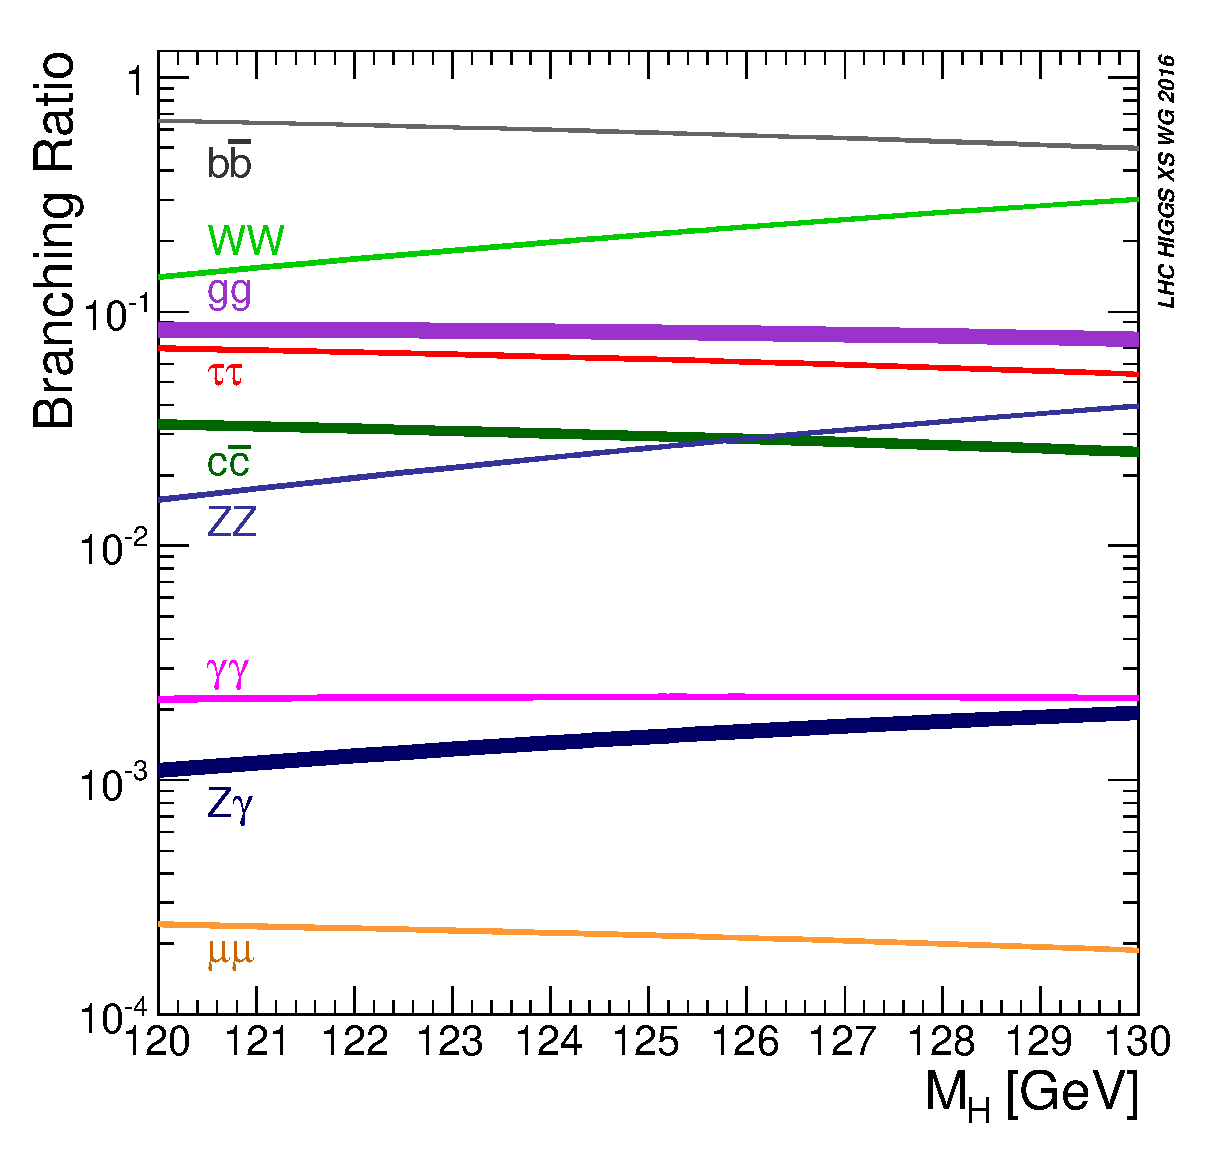
\includegraphics[width=0.5\linewidth]{figures/higgs/higgs_decay_plot.eps}
    \caption{Branching ratios for the decay of the SM Higgs boson near $m_{H} = 125$GeV including theoretical uncertainty bands \cite{PDG2018:Ch11}}
    \label{fig:higgs_decay_plot}
  \end{center}
\end{figure}



\section{Evidence for the SM Higgs} \label{sec:higgs:higgs_evidence}

Using the above information about predicted final states the CMS and ATLAS
experiment collaborations analyszed 5 $\text{fb}^{-1}$ of LHC Run 1 data 
\cite{Khachatryan:2016vau} to make measurements of the SM Higgs production 
cross-sections and branching ratios.  The combined results of these studies 
can be seen in \cref{fig:higgs_production_measurement} 
\cref{fig:higgs_decay_measurement_1} and \cref{fig:higgs_decay_measurement_2}.  
Given the uncertanties on the measurements these results show good agreement 
between the predictions of the Standard Model and experiment with all best 
fit values falling within $2\sigma$ of the SM theoretical prediction.

\begin{figure}[!htbp]
  \begin{center}
    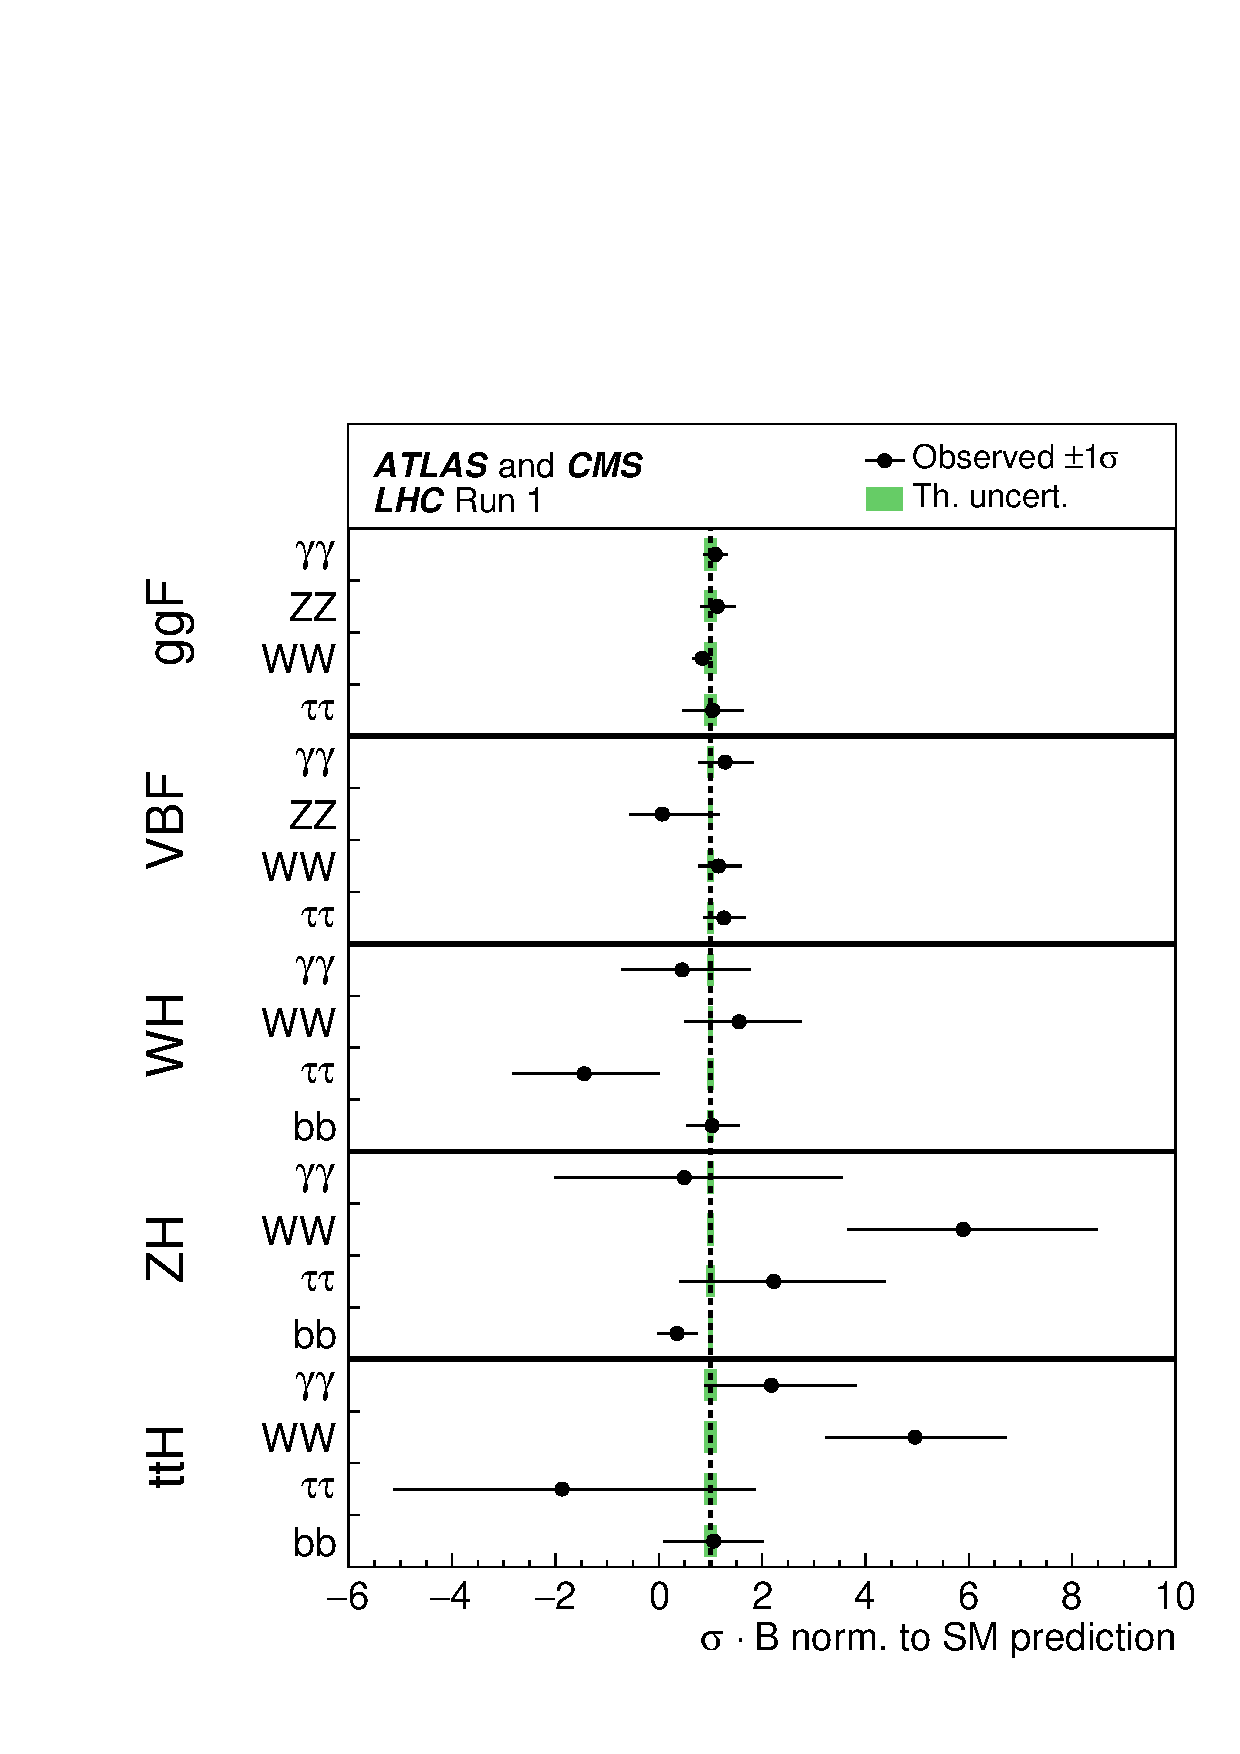
\includegraphics[width=0.5\linewidth]{figures/higgs/higgs_production_measurement.pdf}
    \caption{ Best fit values of $\sigma_{i} \cdot B^{f}$ for each specific channel $i \rightarrow H \rightarrow f$, as obtained from the generic parameterisation with 23 parameters for the combination of the ATLAS and CMS measurements. The error bars indicate the $1\sigma$ intervals. The fit results are normalised to the SM predictions for the various parameters and the shaded bands indicate the theoretical uncertainties in these predictions. Only 20 parameters are shown because some are either not measured with a meaningful precision, in the case of the $H \rightarrow ZZ$ decay channel for the $WH$, $ZH$, and $t\bar{t}H$ production processes, or not measured at all and therefore fixed to their corresponding SM predictions, in the case of the H → bb decay mode for the ggF and VBF production processes \cite{Khachatryan:2016vau}.}
    \label{fig:higgs_production_measurement}
  \end{center}
\end{figure}

\begin{figure}[!htbp]
  \begin{center}
    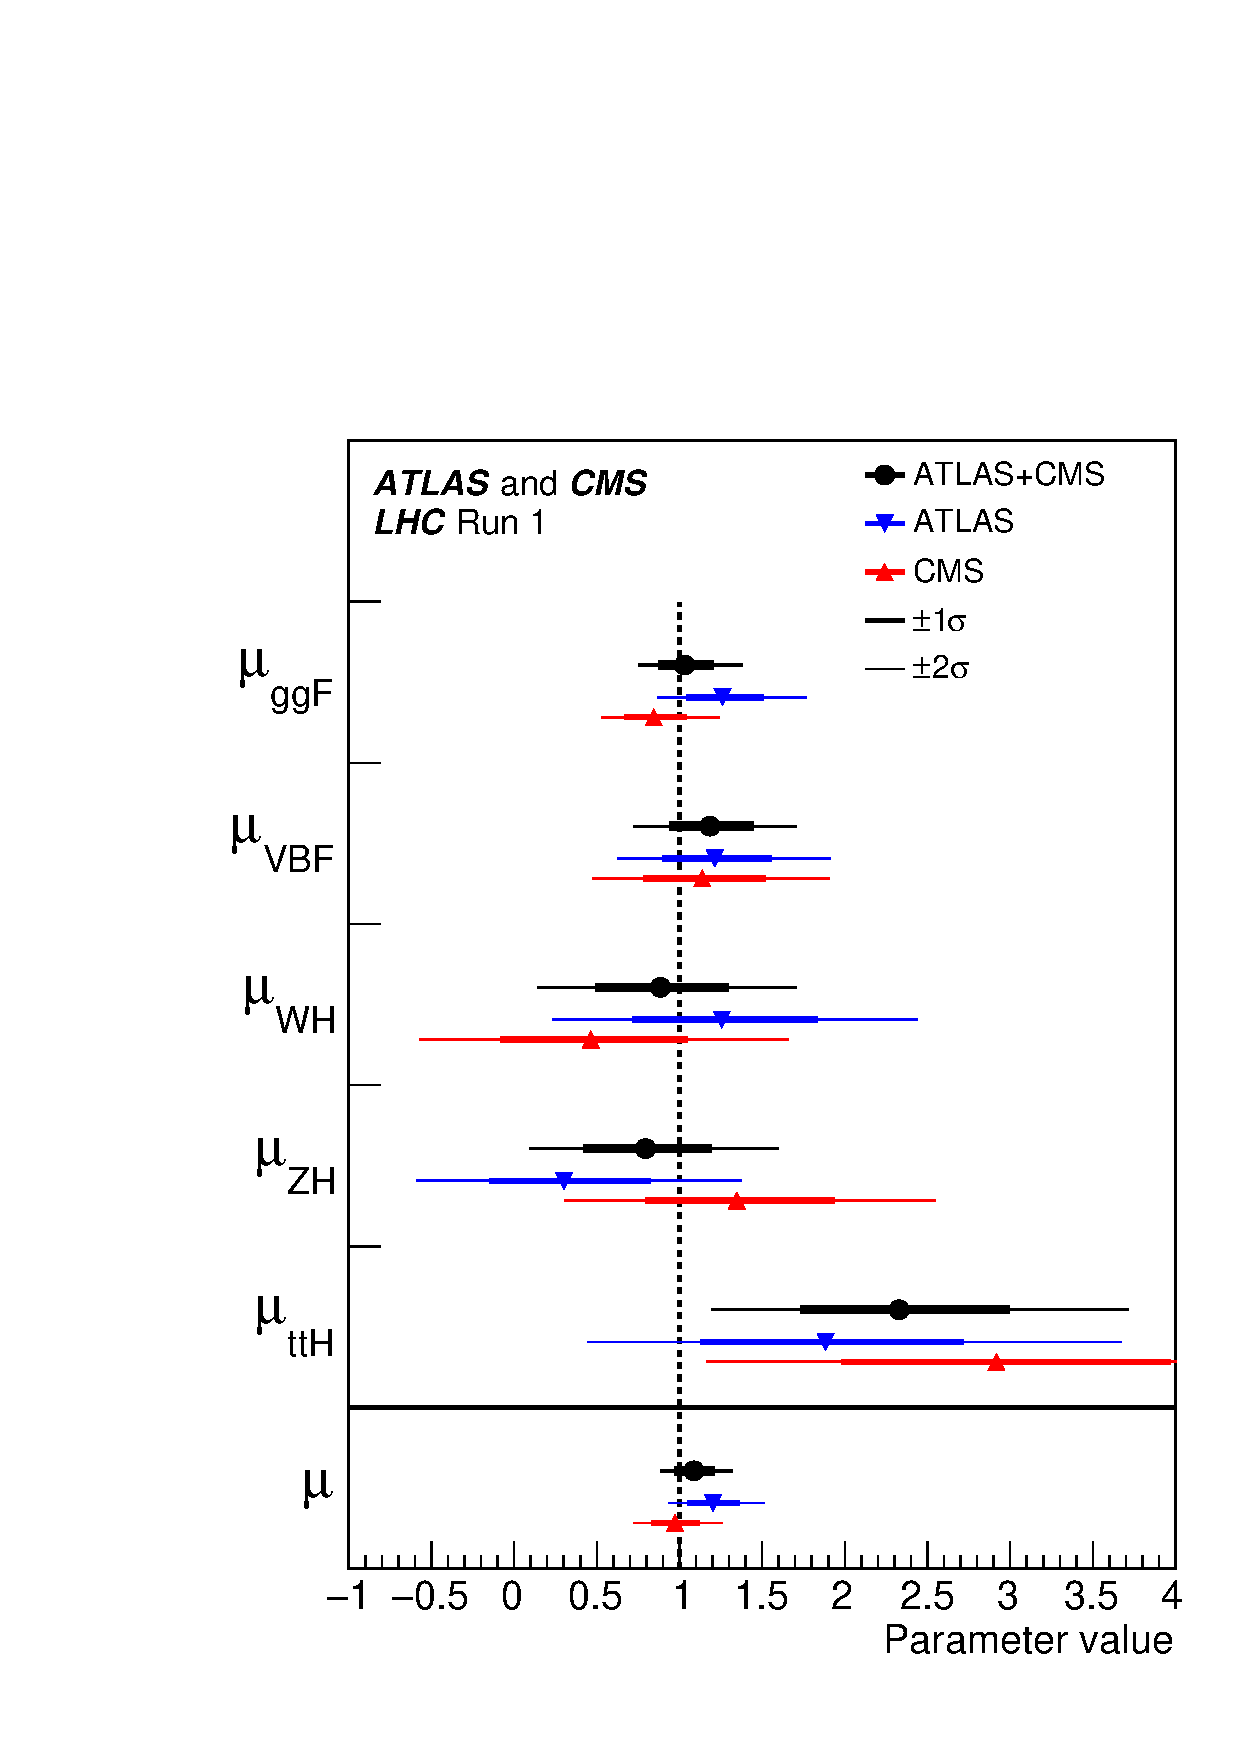
\includegraphics[width=0.5\linewidth]{figures/higgs/higgs_decay_measurement_1.pdf}
    \caption{Best fit results for the production signal strengths for the combination of ATLAS and CMS data. Also shown are the results from each experiment. The error bars indicate the $1\sigma$ (thick lines) and $2\sigma$ (thin lines) intervals. The measurements of the global signal strength $\mu$ are also shown \cite{Khachatryan:2016vau}.}
    \label{fig:higgs_decay_measurement_1}
  \end{center}
\end{figure}

\begin{figure}[!htbp]
  \begin{center}
    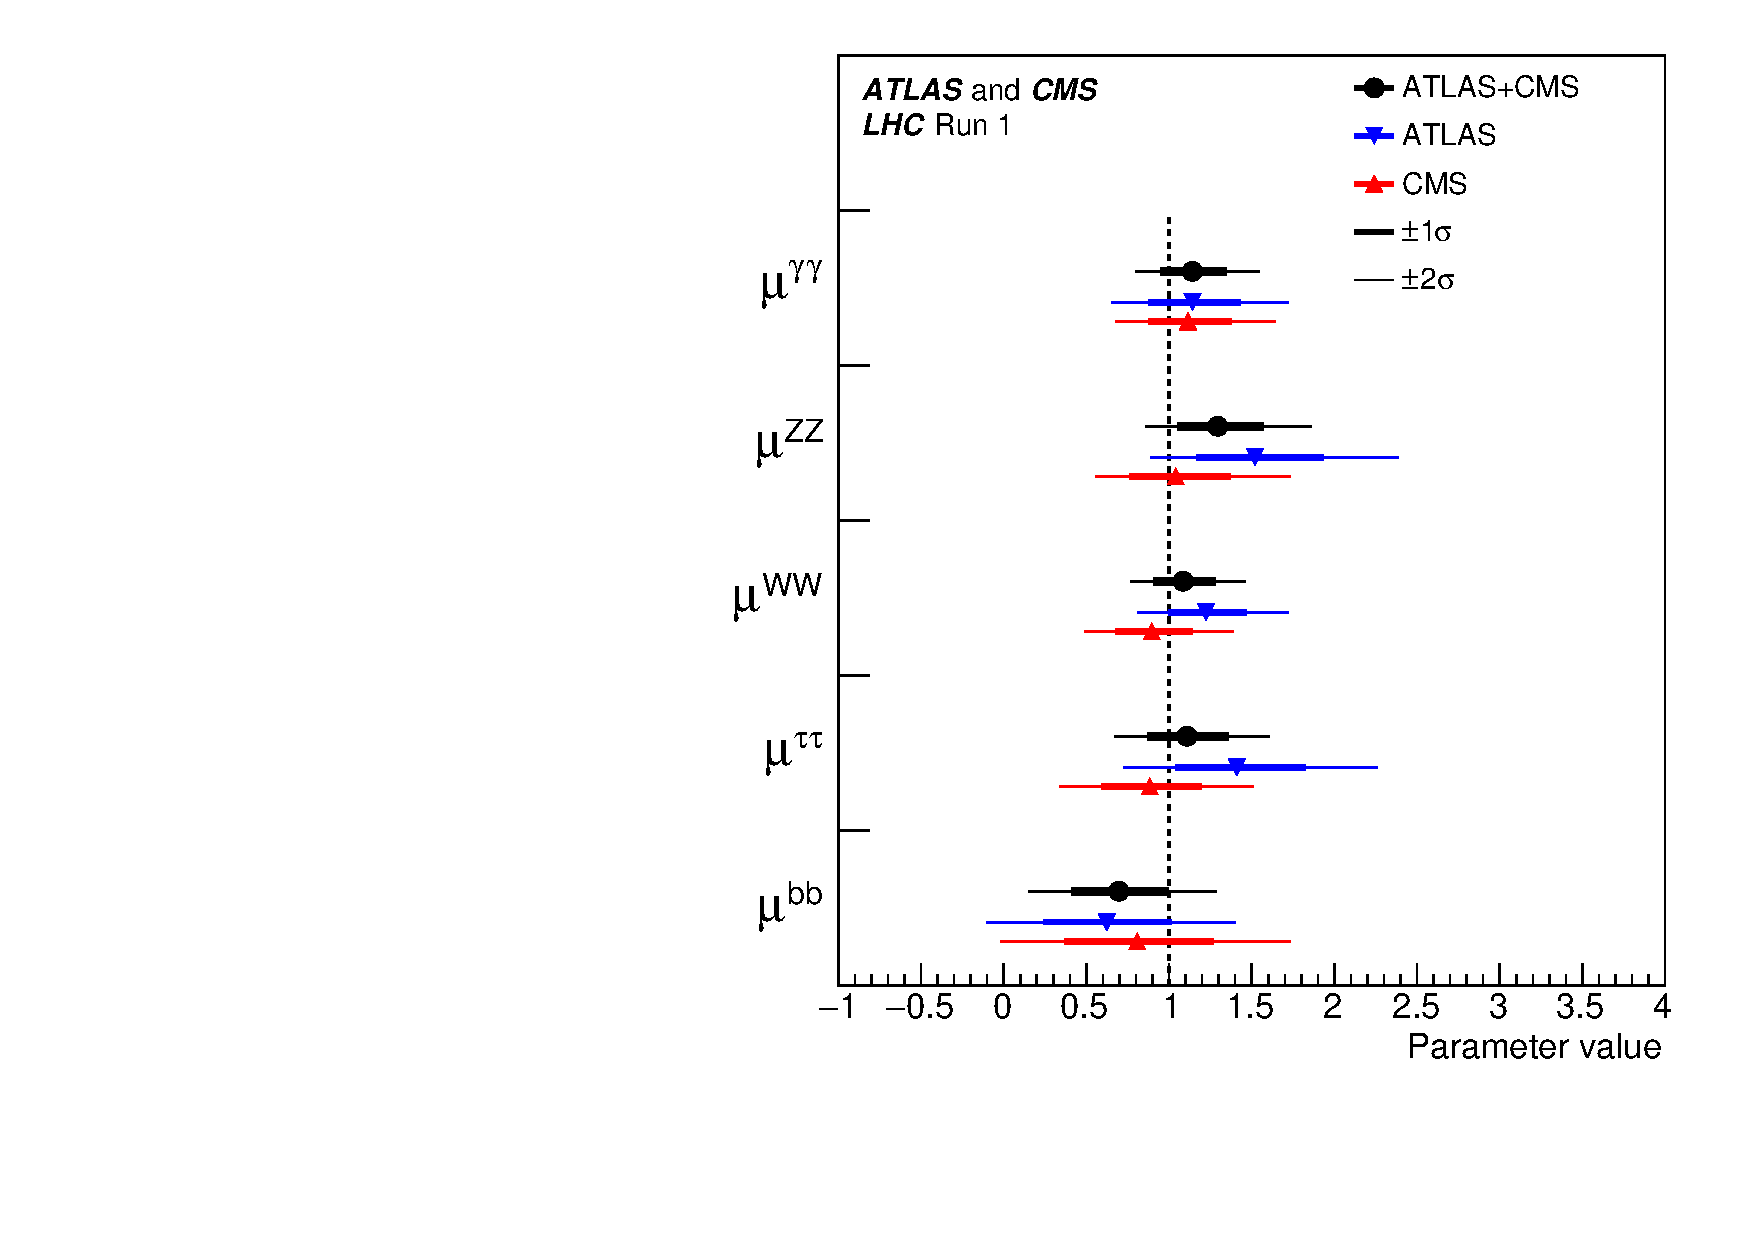
\includegraphics[width=0.5\linewidth]{figures/higgs/higgs_decay_measurement_2.pdf}
    \caption{ Best fit results for the decay signal strengths for the combination of ATLAS and CMS data. Also shown are the results from each experiment. The error bars indicate the $1\sigma$ (thick lines) and $2\sigma$ (thin lines) intervals \cite{Khachatryan:2016vau}.}
    \label{fig:higgs_decay_measurement_2}
  \end{center}
\end{figure}

\section{Boosted Higgs} \label{sec:higgs:boosted}



\part{Experimental Apparatus and Associated Facilities}
% The Large Hadron Collider and ATLAS Detector

\chapter{The Large Hadron Collider} \label{chap:lhc}

Located 100 meters under the Swiss / French boarder lies the 26.7 kilometer
Large Hadron Collider (LHC) \cite{Evans:2008zzb}.  The culmination of a huge international collaboration,
this apparatus is used to produce proton and heavy ion collisions for observation by
the four major experiments at the LHC: ATLAS, CMS, LHCb, and ALICE.  The system
was designed for a maximum center-of-mass  energy of $\sqrt{s} = 14$ TeV and a peak
instantaneous luminosity of $L = 10^{34} $cm$^{-2} $s$^{-1}$.  

The first LHC workshop was held in 1984 in Lausanne at the European Organization
for  Nuclear Reserach (CERN) \cite{LlewellynSmith:2014lmn}.  The nearly 30 year
old case for a machine that would push towards the discovery of the elusive
Higgs Boson was presented using the existing CERN accerlerator facilities and
the Large Electron Positron (LEP) collider tunnel. The proposal became reality
on September 10, 2008 when the first proton beams were circulated, only to have
calamity strike 9 days later in the form of a catastrophic electrical fault. The
repairs and improvements lasted until November 2009 when the LHC restarted.
Since then this modern marvel has worked wonderfuly and, as hoped, lead to the
discovery of the Higgs Boson by the CMS and ATLAS collaborations July 4, 2013.

The following  chapter provides a brief introduction to the worlds
most powerful accelerator starting with the little red bottle of hydrogen in 
building XXX, and ending with the interaction point where protons collide at the 
highest energies ever produced.

\section{Particle Incjecton Chain} \label{sec:lhc:injection}

\begin{figure}[!htbp] 
  \begin{center}
    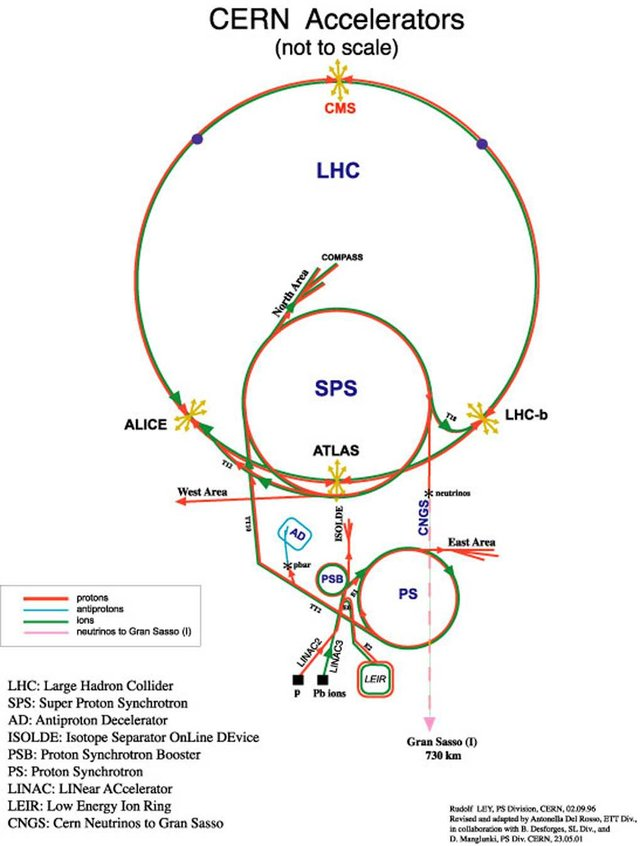
\includegraphics[width=0.9\linewidth]{figures/lhc/injection.jpg}
    \caption{ CERN accelerator complex} 
    \label{fig:injection_chain} 
  \end{center} 
\end{figure}

We begin with the most common element in the Universe, hydrogen, as our source
of protons.  A bottle of hydrogen gas provides 100 microsecond pulses of raw
$H_{2}$ which is then injected into a Duoplasmatron. There,  a strong electric
field and free elctrons from a cathode ionize the molecule into bare $H^{+}$ aka
a proton!  These protons are then accelerated by a 90kV field, leaving the
Duoplasmatron with 1.4\% speed of light ($\sim$4000km/s) or, in relativistic
units, about 83keV. The bare protons are then fed into the accelerating
RadioFrequency (RF) cavities of Linear Accelerator 2 (LINAC2). Inside,
conductors charged by a powerful oscillating electromagnetic field accelerate
the protons resulting in a 50MeV energy. Along the way, small quadrupole magnets
shape the proton packet insuring they remain in a tight beam.  This pattern of
accleration with RF cavities and shaping/turnig with magnets is then repeated
with CERN's first synchrotron, the Proton Synchrotron (PS) rendering a 1.4 GeV
beam.  The final step before the LHC comes with the Super Proton Synchrotron
where the same technologies are implemented to produce 450 GeV protons, ready
for injection into the LHC. A diagramatic representation of this chain can be
seen in figure \cite{injection_chain} 

In order to produce proton-proton collisions the LHC uses two beams circulating
in opposite directions.  The beams are not continuous, but instead consist of
bunches, or buckets, of $\mathcal{O}(10^{11})$ protons with a spacing of 25ns.
Given the LHC circumference this allows for 3564 buckets, however only 2808 are
filled per beam due to safety requirements and injection limitations.  Each beam
takes 4 minutes and 20 seconds to fill and then an additional 20 minutes to for
the protons to reach their maximum energy of 7 TeV TeV, or 99.99999991\% the
speed of light! Under normal operating conditions these beams can be used for
many hours.

\section{Accelerator complex layout and design} \label{sec:lhc:layout}

We begin with the most common element in the Universe, hydrogen, as our source
of protons.  A bottle of hydrogen gas provides raw $H_{2}$ which is then
injected into a Duoplasmatron which uses a strong electric field to break the
molecule into bare $H^{+}$ aka a proton!  The proton is then accelerated by a 90
kV supply and leaves the Duoplasmatron with 1.4\% speed of light (~4000
km/s).


\section{Performance} \label{sec:lhc:performance}

Since the begining of its stable running in 2010 the LHC has performed well,
even exceeding our expectations.  While the experiment itself is incredibly
complex, the performance of the machine, for the purposes of our analysis, can
be reduced to two numbers; the familiar center of mass energy of the beams and a
less common quantity known as the integrated luminosity.  

For particle physics the integrated luminosity is proportional to the total
number of collisions recorded during a specified time period, while the
instantaneous luminosity is proportional to the bunch crossing rate along with
the cross section of a proton-proton interaction and represents the potential
number of collisions per second.  Knowing this we can see that the integrated
luminosity, $L_{int}$ is simply the integral of the instantaneous luminosity
$L_{inst.}$ for a choosen data period as seen in equation XXX.

$$ L_{int} = \int L_{inst.}dt $$

For a standard Gaussian beam, $L_{inst.}$ can be written as

$$ L = \frac{N_{b}^{2}n_{b}f_{rev}\gamma_{r}}{4\pi\epsilon_{n}\beta^{*}}F $$,

where $N_{b}$ is the number of particles per bunch, $n_{b}$ the number of
bunches per beam, $f_{rev}$ the revolution frequency, $\gamma_{r}$ the
relativistic gamma factor, $\epsilon_{n}$ the normalized transverse beam
emittance, $\beta^{*}$ the beta function at the collision point, and $F$ the
geometric luminosity reduction factor due to the crossing angle at the
interaction point given by

$$ F = \bigg(1 + \Big( \frac{\theta_{c}\sigma_{z}}{2\sigma^{*}} \Big) ^{2}
\bigg)^{-1/2} $$,

where $\theta_{c}$ is the full crossing angle at the interaction point,
$\sigma_{z}$ is the RMS bunch length, and $\sigma^{*}$ is the transverse RMS
beam size at the interaction point.

For the ATLAS experiment the integrated luminosity for each year can be seen in
figure XXX as well as an example of the instantaneous luminosity for the choosen
year in figure XXX.

\section{Pile-up at the LHC} \label{sec:lhc:pileup}

Given the large number of protons per bunch and the cross-section of a
proton-proton interaction, the probability to observe multiple interactions per
bunch crossing is quite high.  These multiple-interaction are known as pile-up,
$\mu$ or the time averaged representation $\langle \mu \rangle$, and come in two
different forms: 

\begin{enumerate} \item \textbf{In-time pile-up:} These are the other
proton-proton collisions that occur during the same bunch crossing as the
primary interaction that cauesd the Data Aquisition (DAQ) system to trigger.
These are the standard extra interactions we expect to observe as stated above.
\item \textbf{Out-of-time pile-up:} These are interactions that occur either
before or after a bunch crossing that causes the DAQ to trigger.  This effect is
generally due to the long integration times of some detector electronics.
\end{enumerate}

The pile-up profile for past years can be seen in figure XXX.  The width of this
distributino is due a combination of Poisonian statistics, the decrease in
number of protons per bunch over the lifetime of a single run, and optimization
tweaks to the beam's profile during runtime.  Understanding and eliminating the
noise from these pile-up events is crucial to reconstructing physics variables
to represent the primary interaction we hope to observe.


\chapter{The ATLAS Detector} \label{chap:atlas}

\section{Tracking with the Inner Detector} \label{sec:atlas:tracking}

With its closest component, the Insertable B-Layer (IBL)
\cite{Potamianos:2209070}, only 3.3 cm from the interaction point. The Inner
Detector (ID), shown in \cref{fig:inner_detector_diagram}
\cite{ATLAS-TDR-4,ATLAS-TDR-5}, faces the incredible challenge of providing
precise momentum resolution and identification of both primary and secondary
vertex measurements of charged particle tracks all while receiving the highest fluence.

\begin{figure}[!htbp]
  \begin{center}
    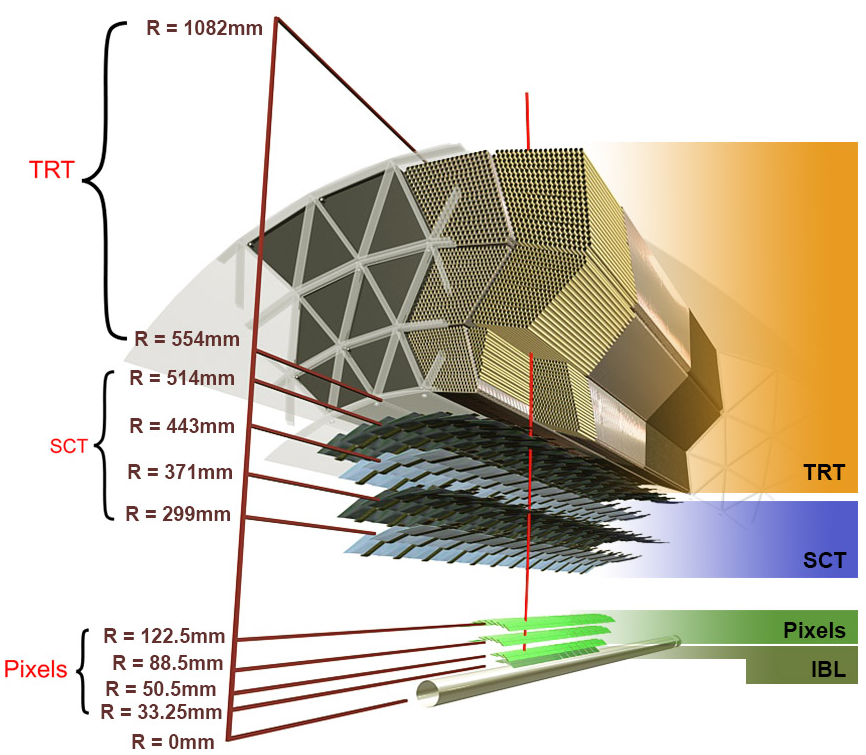
\includegraphics[width=0.8\linewidth]{figures/atlas/inner_detector_diagram}
    \caption{ \cite{Potamianos:2209070} Diagram of inner detector}
    \label{fig:inner_detector_diagram}
  \end{center}
\end{figure}

It is designed to be very compact to reduce the probability of a particle
decaying inside and to give precision measurements of the particles curvature in
the 2T solenoidal magnetic field. This leads to excellent momentum resolution
above the nominal \pT threshold of $0.5$GeV and within the pseudorapidity range
of $|\eta| < 2.5$ as shown in \cref{fig:inner_detector_schematic}.

\begin{figure}[!htbp]
  \begin{center}
    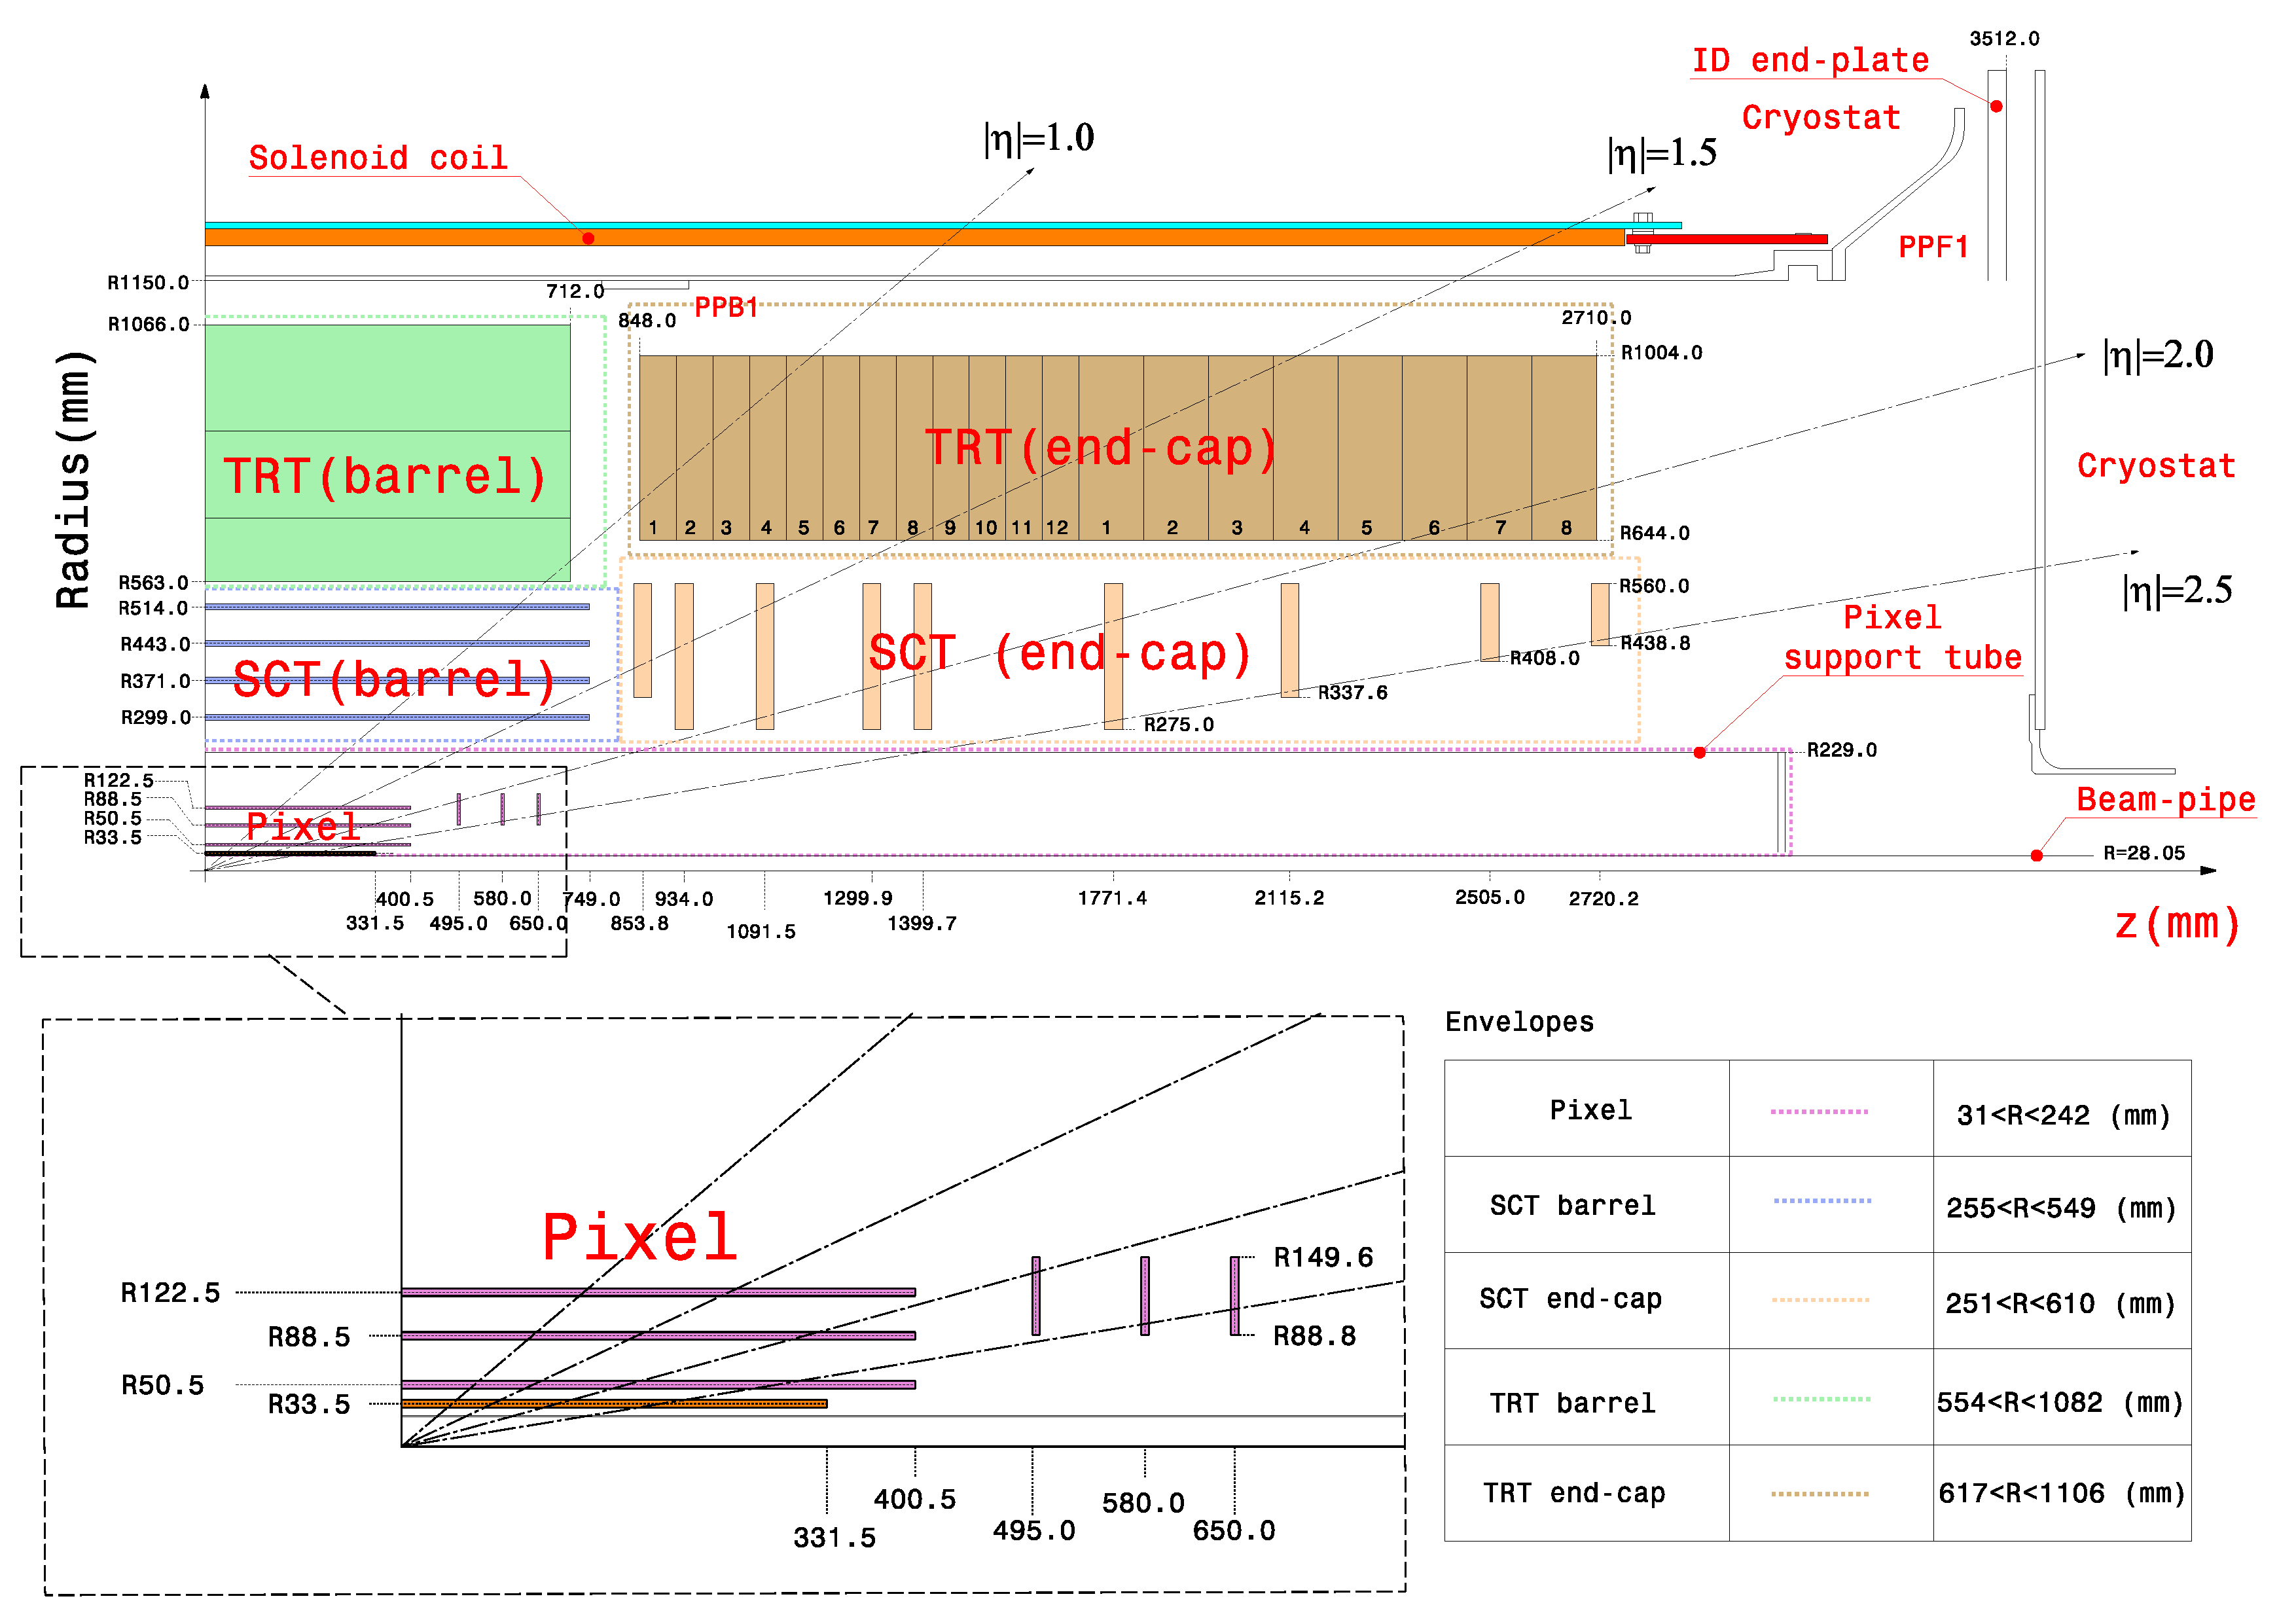
\includegraphics[width=0.8\linewidth]{figures/atlas/inner_detector_schematic}
    \caption{ \cite{PIX-2018-001} Schematic of the Inner Detector including $\eta$
lines.  Each component shown is cylindrically symmetric leading to a
multi-layered detector.}
    \label{fig:inner_detector_schematic}
  \end{center}
\end{figure}

The ID is composed of three different detector technologies for particle
trajector reconstruction: Pixel Detector, Semiconductor Tracker (SCT) and
the Transition Radiation Tracker (TRT).  These will be discussed in the
following sections. 

\subsection{Pixel Detector}

The ATLAS Pixel Detector \cite{PERF-2007-01}, the innermost subdetector of the ID, is designed to
give the best resolution possible as close as possible to the interaction point.
This is accomplished using the 4 barrel layers and 3 disks per endcap as
indicated in \cref{fig:inner_detector_schematic}. The innermost barrel
layer, the IBL, has pixel dimensions of $50\mu $m$(\hat{\phi}) \times 250\mu $m$
(\hat{z}) \times 200\mu $m$(\hat{r})$.  For the other layers the dimensions are
$50\mu $m$(\hat{\phi}) \times 400\mu $m$(\hat{z})$ for about $90\%$ of the pixels
and $50\mu $m$(\hat{\phi}) \times 600\mu $m$(\hat{z})$ for the others, all with a
thickness of $250\mu $m$(\hat{r})$.  This gives a total active area of $1.88 $m$^2$
collected through 92.4 million readout channels, more than half of the total
number of channels for ATLAS. This detailed charged particle information very
close to the interaction point is crucial not only for pattern recognition and
track reconstruction, but also for the reconstruction of the primary and
secondary verticies intrinsic to the decay of $b$-hadrons, a critical element
of the analysis presented in this thesis.

\subsection{Semiconductor Tracker}

Encompassing the Pixel Detector, the Semiconductor Tracker (SCT)
\cite{PERF-2007-01} is composed of double-sided silicon microstrip modules.
Each side of the 4088 modules is constructed out of two silison strip sensors
that are daisy-chained togeather.  The result is 768 composite strips each
$12.6$cm with an inter-strip pitch of $80 \mu$m. In the barrel the strips are
alligned with the $\hat{z}$ direction, while in the end-caps they are aligned
with the $\hat{r}$ direction. In both cases the separation of the strips is
constant in $\hat{\phi}$. The two sides are rotated with respect to each other
by $40 \mu$m to allow for position measurement along the length of the strip.
These modules are then used to tile the 4 barrel layers and 9 disks per endcap
(18 disks in total) as seen in \cref{fig:inner_detector_schematic}.  This
design is chosen to ensure that each charged track interacts with 8 strip
layers (equivalent to four space points).  This information is used to further
measure the momentum and impact parameter, as well as vertex identification of
charged particles.

\subsection{Transition Radiation Tracker}

The Transition Radiation Tracker \cite{PERF-2007-01}, the outermost subdetector
of the ID, provides tracking through the detection of transition radiation from
ultra-relativistic charged particles for $\eta < 2.0$ using 350,000 drift tube
channels also known as straws.  The 4mm diameter straws are filled with a $70\%$
Xe, $27\%$ CO$_2$, and $3\%$ O$_2$ gas mixture and a 31$\mu$m diameter
gold-plated tungsten wire anode at the center for the collection of the
ionization signal. In the barrel 73 azimuthally symetric layers of 144cm straws
are oriented parallel to the beam pipe with an electrical division in the center
of each allowing the two sides to be read out separately.  For each endcap the
straws are radially oriented in 160 symmetric planes each containing 768 37cm
long drift tubes shown in \cref{fig:inner_detector_schematic}.  In both
the barrel and the endcaps polypropylene fibers (barrel) or foils (encaps)
function as the transition radiation material which causes the relativistic
charged particles to radiate and thus ionize the gas in the straw.  The amount
of transition radiation produced is proportional to the Lorentz factor meaning
that lighter particles (e.g. electrons) will produce more radiation.  Thus, by
defining a high and low threshold, we can identify tracks belonging to electrons
by requiring they register more high-threshold hits. There are typically 36 TRT
hits per charged particle track. 

\section{Calorimetry} \label{sec:atlas:calorimetry}

\begin{figure}[!htbp]
  \begin{center}
    \includegraphics[width=0.8\linewidth]{figures/atlas/calorimeter_cutaway}
    \caption{ \cite{PERF-2007-01} A cutaway diagram of ATLAS's sampling calorimeters}
    \label{fig:calorimeter_cutaway}
  \end{center}
\end{figure}

Once the proton collision remnants have passed through the ID and it's
surrounding solenoid they enter into the ATLAS calorimeters depicted in figure
\ref{fig:calorimeter_cutaway}.  Sampling calorimeter technologies were choosen
for their compact geometry and lower cost point.  These are constructed by
alternating layers of absorber, a dense material which reduces the incedent
particles energy, and active material which produces a detectible signal when a
partilce passes through.  This means that the detected signal is only a fraction
of the total energy of the particle and thus requires a study of the calorimeter
response for calibration purposes \cite{Fabjan:692252}. The first system, the
Electromagnetic Calorimeter (EMC), is designed to measure the energy of
electrons and photons which primarily lose their energy via bremstralung and
pair production electromagnetic interactions.  Outside of the EMC is the
Hadronic Calorimeter (HC) which is designed to measure the energy of jets of
hadrons through their electromagnetic and strong interactions. These detectors
cover the entire $|\eta| < 4.9$ range and provide complete containment of both
Electromagnetic and Hadronic showers with higher granularityi in the EMC for
$|\eta| < 2.5$, the region matched to the ID, for precision measruements of
electrons and photos.  By instrumenting this huge space in $|\eta|$ we can
search for events with asymetric energy deposits which imply the existence of a
particle we didn't detect represented by missing transverse energy $\MET$.

\subsection{Electromagnetic Calorimeter}

The innermost calorimeter, the Liquid Argon (LAr) Electromagnetic Calorimeter
(EMC) \cite{PERF-2007-01}, uses lead as the absorber and liquid argon as
the active material in an "accordion geometry" as seen in figure
\ref{fig:accordion}. This geometry was choosen for uniform coverage in
$\hat{\phi}$ due to its lack of un-instrumented cracks in the radial direction.
The barrel region covers $|\eta| < 1.475$ and an end cap on each side covers
$1.375 < |\eta| < 3.2$ each housed in their own cryostat.  The barrel is
composed of two half barrels with a 4mm gap at $z = 0$ and both end caps are
divided into an intter wheel covering $2.5 < |\eta| < 3.2$ and an outer wheel
covering $1.375 < |\eta| < 2.5$.

\begin{figure}[!htbp]
  \begin{center}
    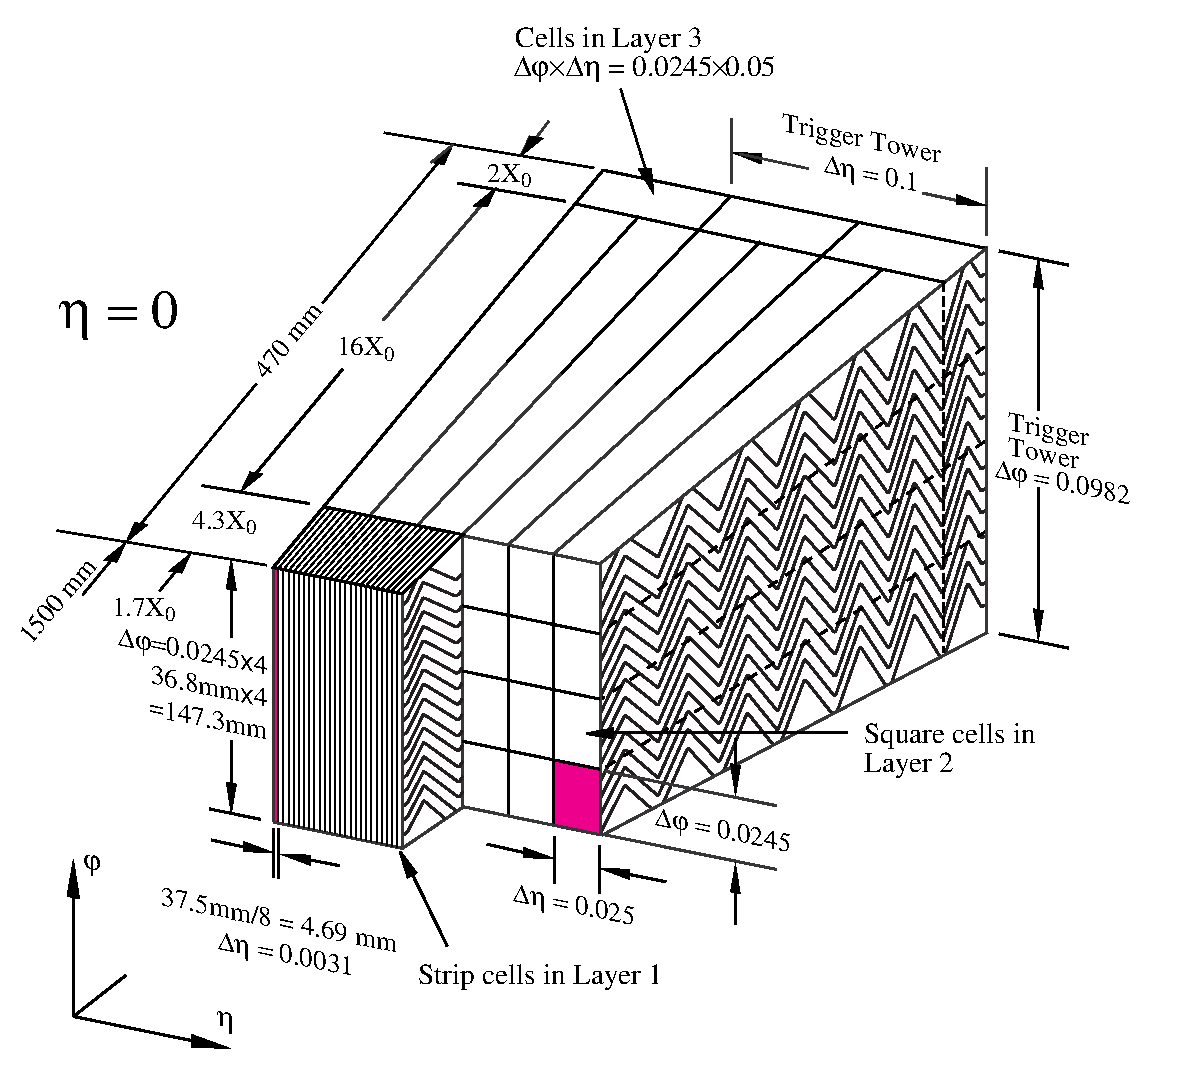
\includegraphics[width=0.8\linewidth]{figures/atlas/accordion}
    \caption{ \cite{PERF-2007-01} Sketch of LAr EMC barrel module where the lead
and liquid argon layers are visible in an accordion like geometry. Looking from
the foreground to the back there are 3 different types of cells visible.}
    \label{fig:accordion}
  \end{center}
\end{figure}

In the $|\eta| < 2.5$ region the EMC has 3 radial layers for precision physics
measurements.  Layer 1 consists of strip cells which are finely segmented with
$\Delta\eta = 0.0031$ and $\Delta\phi = 0.0245$ allowing for precision position
resolution which gives discrimination power between a single $\gamma$ deposit
and the $\pi^0$ characteristic $\gamma\gamma$ deposit. Layer 2 , which collects
the largest fraction of energy from electromagnetic shower, is segmented with
$\Delta\eta = .025$ and $\Delta\phi = 0.0245$. Layer 3 collects the tail of the
electromagnetic shower using a coarser segmentation of $\Delta\eta = .05$ and
$\Delta\phi = 0.0245$.  Additionally, in the region $|\eta| < 1.8$ a thin
pre-sampler , which contains no lead absorber, was placed in front of Layer 1 to
allow for energy corrections due to losses upstream of the EMC.  Combined the
EMC is $>$ 22 radiation lengths ($X_0$) in the barrel and $>$ 24 $X_0$ in the
end-caps, where a radiation length is the average distance an electron travels
in a given material before losing $1/e$ of its original energy $E_0$ via
bremsstrahlung radiation.

\subsection{Hadronic Calorimeter}

Directly outside the EMC envelope is the Hadronic Calorimeter (HC) system
\cite{PERF-2007-01} which consists of three sampling calorimeter technologies:
the Tile calorimeter, the LAr hadronic end-cap calorimeter (HEC) and the LAr
forward calorimeter (FCal).  Combined, these three subsystems give measurements
of hadronic jet energies in the $0 <|\eta| < 4.9$ range. The tile calorimeter
uses steel as the absorber layer and scintillating tiles as the active material
and covers the region $|\eta| < 1.7$ with a barrel section flanked by two barrel
extensions each divided azimuthally into 64 modules.  These scintillator tiles
are read out on two sides by wave-length shifting fibers connected to
photomultiplier tubes as seen in figure \ref{fig:tile_calorimeter}. At $\eta =
0$ the total tile calorimeter thickness is 9.7 nuclear interaction lengths
($\lambda$), where $\lambda$ is the average distance a hadron travels before
interacting inellastically with a nucleus.

\begin{figure}[!htbp]
  \begin{center}
    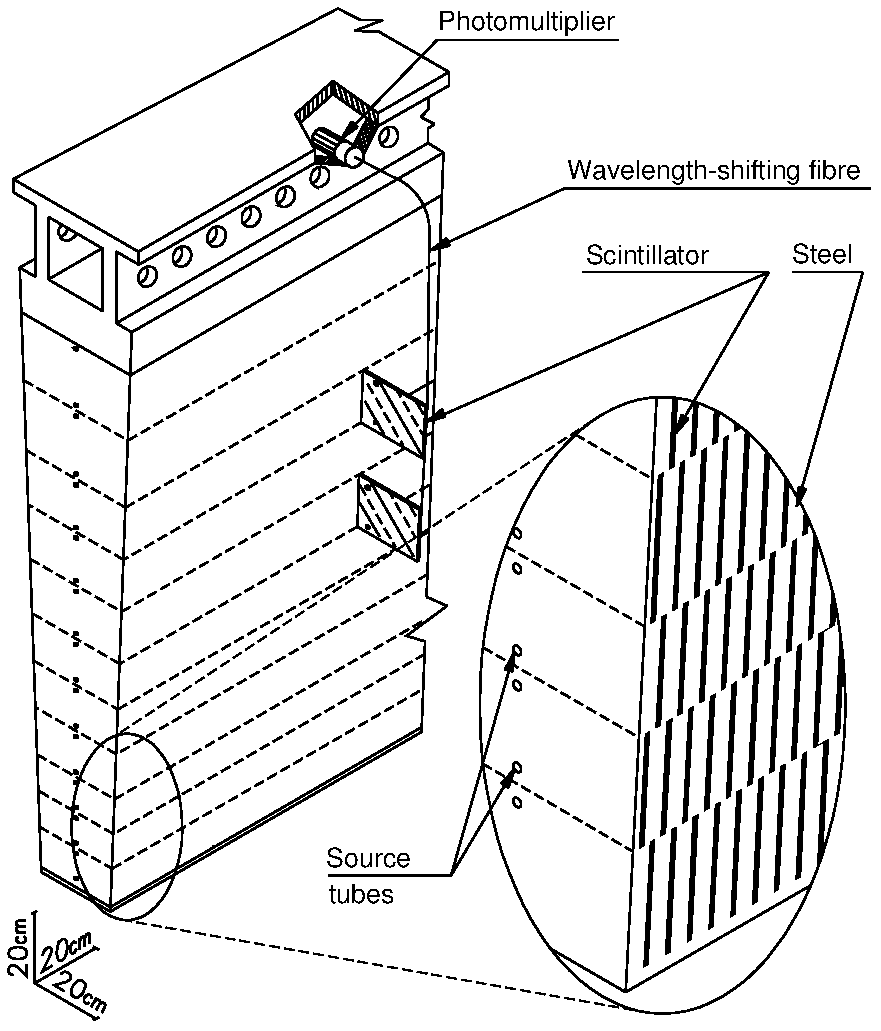
\includegraphics[width=0.8\linewidth]{figures/atlas/tile_calorimeter.pdf}
    \caption{ \cite{PERF-2007-01} Schematic of a tile calorimeter module
including a depiction of the connection between the scintillator tile to the
photomultiplier via a wavelength-shifting fibre.}
    \label{fig:tile_calorimeter}
  \end{center}
\end{figure}

The HEC is composed of two independent wheels per end-cap located just past the
EMC end-cap but sharing the same cryostat. This system  uses copper as an
absorber and liquid argon for the active material and covers the $1.5 < |\eta| <
3.2$ range using 32 wdge-shaped modules per wheel. Finally, the FCal shares the
same cryostat as the EMC and HEC end-caps and acts to extend the coverage of the
combined calorimeter system to include the $3.1 < |\eta| < 4.9$ range.  Each
endcap contains 3 modules, the first an electromagnetic module
(Copper/Liquid-Argon) which is followed by two hadronic modules which use
(Tungsten/Liquid-Argon.

\section{Muon Spectrometer} \label{sec:atlas:muons}

The ATLAS Muon Spectrometer (MS) \cite{PERF-2007-01}, see
\Cref{fig:muon_system}, accomplishes tracking of muons in the $|\eta| < 2.7$
region for momentum reconstruction while also triggering on charged particles
in the $|\eta| < 2.4$ region.  The magnetic field necessary for momentum
reconstruction is provided by 3 air-core toroid systems, one barrel toroid
covering $|\eta| < 1.4$ and two end-cap toroid systems which are inserted into
the inner radius of the barrel toroid to cover the $1.6 < |\eta| < 2.7$. The
so-called transition region $1.4 < |\eta| < 1.6$ between these two magnet
systems is covered by a combination of the barrel and end-cap toroid magnets.
Similar to the ID the resolution in the MS is inversely proportional to the particle's
incident momentum.  Any muon with $\pt$ lower than $\sim 3~\GeV$ will never
make it to the MS due to energy loss in the calorimeters \cite{PERF-2007-01}.

\begin{figure}[!htbp]
  \begin{center}
    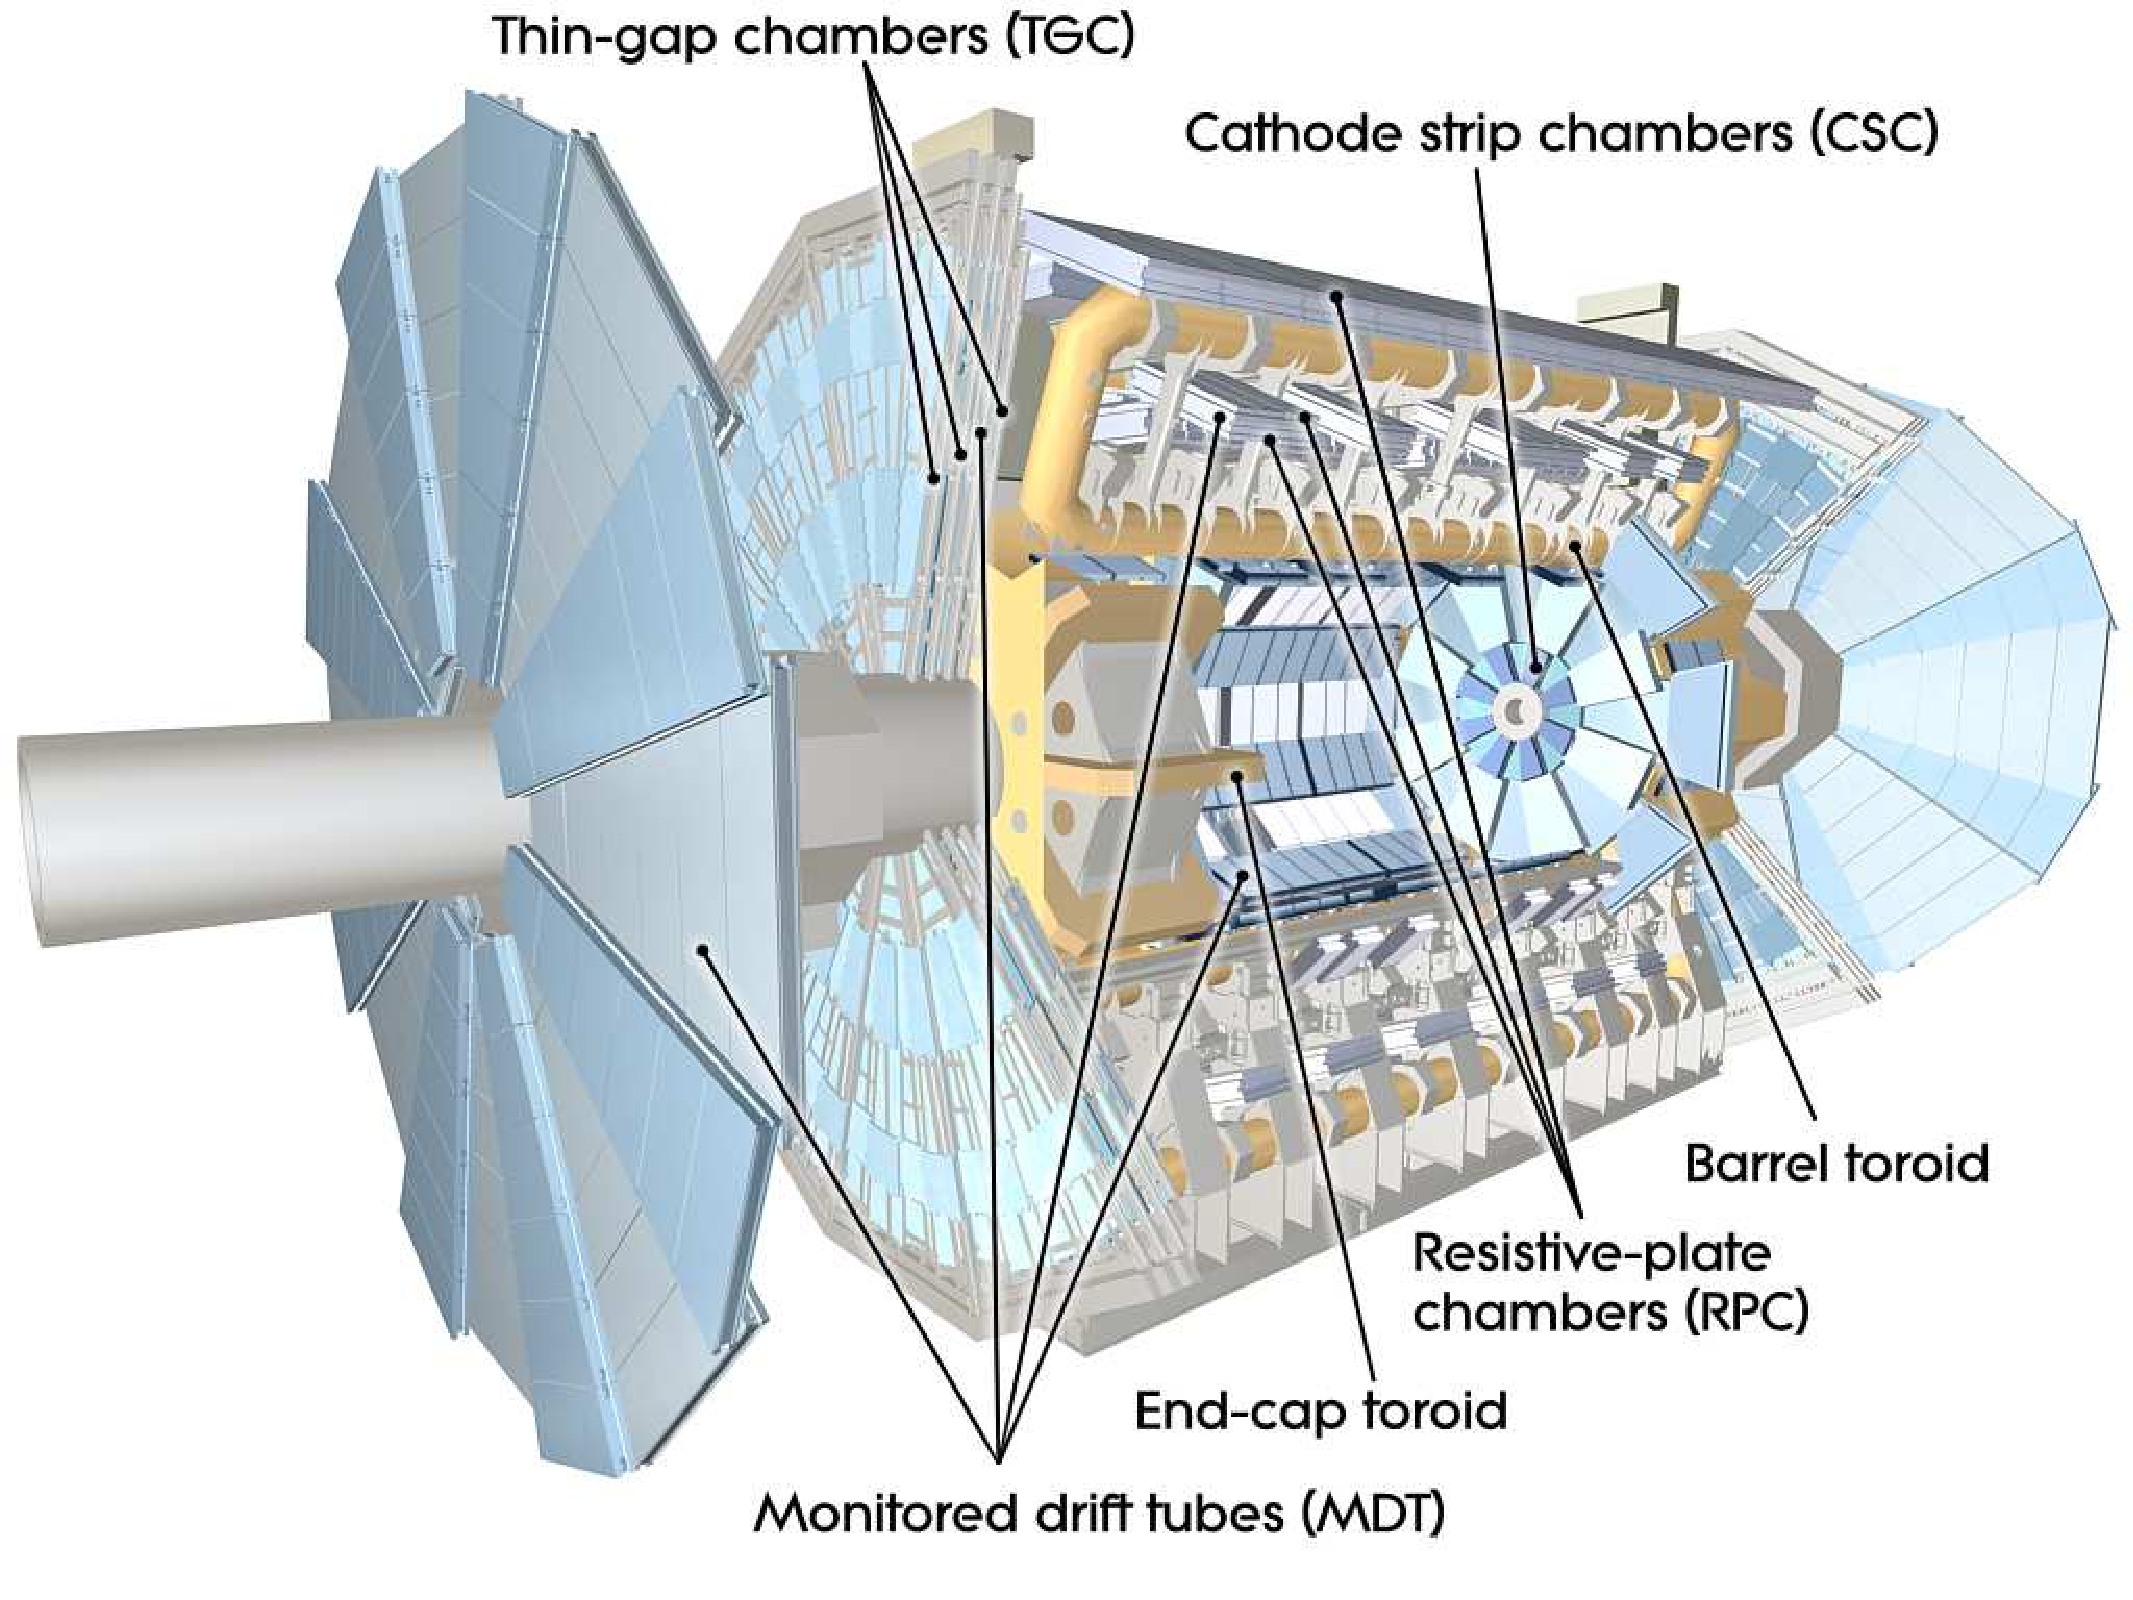
\includegraphics[width=0.8\linewidth]{figures/atlas/muon_system}
    \caption{A cut-away diagram of the ATLAS muon system
and its many sub-detectors \cite{PERF-2007-01}.}
    \label{fig:muon_system}
  \end{center}
\end{figure}

Precision tracking measurements for momentum reconstruction is accomplished
using the Monitored Drift Tube chambers (MDTs) for $|\eta| < 2.0$.  The MDT
system consists of 1163 drift tube chambers arranged in three to eight layers
for varying $\eta$.  The Cathode-Strip Chambers (CSCs) span the range $2.0 <
|\eta| < 2.7$ and are designed to withstand the higher rate at high $\eta$ and
retain good time resolution using multiwire proportional chambers with
orthogonal segmented cathode planes.

The MS also gives nanosecond tracking information for triggering on muon tracks.
This is accomplished using Resistive Plate Chambers (RPC) in the barrel region
$|\eta| < 1.05$ and Thin Gap Chambers (TGC) in the end-cap $1.05 < |\eta| < 2.4$
region.  Both chamber systems deliver a triggerable signal with a spread of
$15-25$ ns, thus providing the ability to tag individual beam-crossings.




\part{The HbbISR Analysis}
% The analysis 

\chapter{Data and Monte-Carlo Simulation} \label{chap:data}

This analysis focuses on the data collected by the ATLAS detector from \pp
collisions produced by the LHC at the center-of-mass-energy of 13 TeV.  In
particular the analysis shown uses datasets collected in 2015, 2016, and 2017
and ammounts to an integrated luminosity of $80.5 \text{ fb}^{-1}$ after beam,
detector and data-quality requirements are taken into account. 

In order to compare our findings with theory, we use the predictions of the SM
to produce Monte-Carlo (MC) simulated events to model the signal and background
processes.  These MC samples go through a full simulation of the ATLAS detector
and are processed such that the MC and Data have the same format at analysis
level. This allows us to analyze the MC and Data using the same framework such 
that we can make direct comparisons between theory and reality as our final product.

\section{Data Used} \label{sec:data:data}

As mentioned earlier, the data are checked to make sure they are of high
quality, meaning that the beam, detector and data collection systems were all
fully operational during the event in question. These data quality requirements
are enforced by choosing only events from each respective year's Good Runs List
(GRL), an XML file produced by the ATLAS data quality monitoring team that
lists all luminosity blocks that have met the data quality criteria.  This
analysis uses three such GRLs - one for each year of data taking
(2015, 2016, 2017) - corresponding to annual integrated luminosities of
$3.2~\ifb$, $33~\ifb$, and $44.3~\ifb$.

\section{Higgs Boson Signal Monte Carlo Samples} \label{sec:data:signal_mc}

In order to simulate Higgs boson events, the three leading production
mechanisms at the LHC were considered, shown in \Cref{fig:higgs_production}:
gluon-gluon fusion, vector boson fusion and Higgsstrahlung.  These three
production modes represent 50\%, 30\% and 20\% of the total Higgs signal,
respectively, before analysis cuts are applied.  In all samples the simulated
Higgs boson is forced to decay to the $b\bar{b}$ final state.

The ggF $H$ + jet events were generated using the HJ+MiNLO~\cite{Hamilton2015}
prescription, assuming a finite top quark mass, with the \textsc{Powheg-Box} 2
generator~\cite{Campbell2012} and the NNPDF30 NNLO parton distribution
functions~\cite{Hamilton:2012rf}.  After generation the events were showered
using \textsc{Pythia} 8.212~\cite{Sjostrand:2014zea} with the AZNLO tune and
the CTEQ6L1 parton distribution functions~\cite{Pumplin:2002vw}. Any
$b$-hadrons produced during this process were decayed using
\textsc{EvtGen}~\cite{LANGE2001152}.

The VBF $H$ + jet events were also generated using the \textsc{Powheg-Box}
generator~\cite{Nason:2009ai} with the NNPDF30 NLO parton distribution
functions~\cite{Hamilton:2012rf}. Again the showering was performed with
\textsc{Pythia} 8.212~\cite{Sjostrand:2014zea} using the AZNLO tune and the
CTEQ6L1 parton distribution functions~\cite{Pumplin:2002vw}.  The decay of
$b$-hadrons was again performed using \textsc{EvtGen}~\cite{LANGE2001152}.

Higgsstrahlung events were generated using the \textsc{Pythia} 8.212
generator~\cite{Sjostrand:2014zea}, the AZNLO tune and the CTEQ6L1 parton
distribution functions~\cite{Pumplin:2002vw}.  Again the decay of $b$-hadrons
is handled by \textsc{EvtGen}~\cite{LANGE2001152}. Unfortunately the
\textsc{Pythia} $ZH$ process does not include the $gg \rightarrow ZH$
contribution.  To account for this the cross section is corrected to the LHC
Higgs cross section working group's (LHCHXSWG) recommendation
\cite{MelladoGarcia:2150771}.

\section{Background Monte Carlo} \label{sec:data:bkg_mc}

Modeling the expected contributions of backgrounds to the analysis is done with
a mix of data driven methods and Monte Carlo simulated samples as discussed in
\Cref{chap:background}.  The MC samples were used for the development of the
modeling of the non-resonant QCD multijet backgrounds and for the estimation
of the major resonant backgrounds from $V$+jet, $t\bar{t}$, and single-top
production.  For the multijet background the final estimation is data driven,
but the MC was used to develop the background model.

The QCD dijet events were simulated by the \textsc{Pythia} 8.186
generator~\cite{Sjostrand:2007gs} with the A14 tune and the NNPDF23 LO
PDF~\cite{Carrazza:2013axa} using \textsc{EvtGen} to decay the resulting
$b$-hadrons~\cite{LANGE2001152}.  To maintain a constant statistical precision
over a large momentum range, the weighted events were generated with a flat \pT
spectrum.

Hadronically decaying $W$ and $Z$ events were produced with a maximum of four
additional partons at leading order (LO).  This was accomplished with the
\textsc{Sherpa} 2.1.1 generator~\cite{Gleisberg:2008ta} and the CT10 parton
distribution functions~\cite{Lai:2010vv}.  For leptonically decaying $W$ and
$Z$ events samples were produced with a maximum of two additional partons at LO
and a maximum of four at next-to-leading order (NLO).  This allowed us to
correct the LO hadronic $W$ and $Z$ cross-sections to the NLO leptonic $W$ and
$Z$ cross-sections by applying multiplicative ``$k$-factors."  These corrections
were 1.28 for the $W$+jets and 1.37 for the $Z$+jets \cite{Aaboud:2018zba}. An
alternate sample of hadronically decaying $W$ and $Z$ events was produced for
cross checks using the \text{Herwig}++2.7.1 generator~\cite{Bahr:2008pv} with
the UEEE4 tune~\cite{Buckley:2018wdv} and the CTEQ6L1~\cite{Pumplin:2002vw}.
Unlike the \textsc{Sherpa} samples these \textsc{Herwig} samples only contained
one additional parton in the matrix element calculation.

Our $t\bar{t}$ samples were generated at tree-level using \textsc{Powheg-Box}
2~\cite{Campbell2012} and the NNPDF30 NLO parton distribution
functions~\cite{Ball:2014uwa}. After generation the events were showered using
\textsc{Pythia} 8.230~\cite{Sjostrand:2014zea} using the A14 tune and the
NNPDF23 LO parton distribution functions~\cite{Carrazza:2013axa} with all
$b$-hadron decays performed by \textsc{EvtGen}~\cite{LANGE2001152}.  The
samples were then broken up according to the decay mode of the two top quarks
into three categories; all-hadronic, semi-leptonic, all-leptonic. Additional
$t\bar{t}$ events were generated with the \textsc{Sherpa} 2.2.1
generator~\cite{Gleisberg:2008ta} using the NNPDF30 NNLO parton distribution
functions~\cite{Ball:2014uwa}.  This second sample was used as a cross check of
the main samples generated with \textsc{Powheg-Box} 2 + \textsc{Pythia} 8.

Single-top samples, containing a single top/anti-top quark and a
$W^{-}$/$W^{+}$, were generated at tree level with \textsc{Powheg-Box}
2~\cite{Campbell2012} with the NNPDF30 parton distribution
functions~\cite{Lai:2010vv}. This process was showered using \textsc{Pythia}
8.230~\cite{Sjostrand:2014zea} configured with the A14 tune and the NNPDF23
parton distribution functions~\cite{Carrazza:2013axa} with all resulting
$b$-hadrons decayed via \textsc{EvtGen}~\cite{LANGE2001152}.


\chapter{Physics Object Selection} \label{chap:objects}

After the ATHENA Digitization step both data and monte carlo have the same
format, representing the three dimentional energy deposits.  In order to analyze
these deposits they are cleaned, clustered and checked for overlap resulting in
physics objects useful for our specific analysis.

\section{Calorimeter Jets} \label{sec:objects:calo_jets}

\section{Track Jets} \label{sec:objects:track_jets}

\section{Fat Jets} \label{sec:objects:fat_jets}

\section{B-tagged Jets} \label{sec:objects:b_jets}

\section{Muons} \label{sec:objects:muons}

As muons traverse the entire detector they leave a track of charge deposits in
the Inner Detector (ID) and Muon Spectrometer (MS) which is then reconstructed to
represent the path of the muon \cite{Aad:2016jkr}. This results in four
different muon types, dependant upon which subdetectors were used in the
reconstruction:

\begin{enumerate}
  \item Combined (CB) muons: First the charged track is reconstructed independently in the ID and MS.  Then a global refit combines the hits from both subdetectors. This global fit may add or subtract MS hits from the track to achieve the best fit quality.
  \item Segment-tagged (ST) muons: A track is developed in the ID and then extrapolated to the MS.  If this extrapolation finds at least one local track segment in the MDT or CSC it is labeled a muon.  This is generally used for low $\pT$ muons which may only traverse one layer of the MS.
  \item Calorimeter-tagged (CT) muons: A track formed in the ID is labeled a muon if it can be associated with a calorimeter deposit consistent with a minimum-ionizing particle.  This is the least pure muon type, but it allows for reconstruction of muons that pass through the partially instrumented region of the MS.
  \item Extrapolated (ME) muons: These muons are reconstructed using only MS track information and the loose requirement that the hits are compatible with a trajectory originating from the interaction point.  This type is useful for extending the muon acceptance into the region not covered by the ID.
\end{enumerate}

After the muon type is determined the quality of the muon is categorized by
requiring a specific number of hits in each subcomponent.  These quality
requirements are provided to address the specific needs of different physics
analysis. The four muon quality levels are defined:

\begin{enumerate}
  \item[\texttt{loose}] The lowest quality is designed to maximize the reconstruction efficiency for muons by allowing all muon types to be used.  This is primarily useful for analyses of multi-leptonic final states such as $H \rightarrow 4\ell$.
  \item[\texttt{medium}] The medium quality is designed to minimize the systematic uncertainties associated with muon reconstruction and calibration.  Only CB and ME tracks are used, with at least 3 CB track hits and at least 3 ME layers.  This is the default quality selection in ATLAS and the one used for muons in this analysis.
  \item[\texttt{tight}] This selection maximizes the purity of muons but reduces the reconstruction efficiency. Only CB muons with at least 2 layers of the MS that also satisfy the \texttt{medium} selection requirements are allowed.
  \item[\texttt{high-$\pT$}] Designed to optimize the momentum resolution for tracks with $\pT > 100~\GeV$.  This selection only includes CB muons with hits in at least two layers of the MS that also satisfy the \texttt{medium} selection requirements. This quality level is mostly used for high-mass $W'$ and $Z'$ analyses.
\end{enumerate}

The final step for muon reconstruction is to check that the muon is well
isolated, in order to suppress muons resulting from meson and heavy-flavor decays. This
is done using both the track-based ($\pT^{\text{varcone}30}$) and the
calorimeter-based ($E_{\text{T}}^{\text{topocone}20}$) isolation-based variables which
represent the scalar sum of $\pT$ inside a $\Delta R < 0.3$ cone and the
scalar sum of $E_{\text{T}}$ inside a $\Delta R < 0.2$ cone.  Taking the ratio of
these variables to the total $\pT$ of the candidate muon gives a sense of
how much radiation is surrounding the core of the muon in question. Many
different isolation working points are established by cutting on these ratio
distributions. For this analysis the \texttt{loose} working point was chosen which gives a
$99\%$ muon reconstruction efficiency constant in $\eta$ and $\pT$ as
measured in both a simulated $Z \rightarrow \mu\mu$ sample and data \cite{Aad:2016jkr}.

After reconstruction, these muons are calibrated to data using the well understood
decay $J/\Psi \rightarrow \mu^{+}\mu^{-}$ to cover the low $\pT$ spectrum and
$Z \rightarrow \mu^{+}\mu^{-}$ for the high $\pT$ spectrum, as shown in \Cref{sec:objects:medium_muons}.

\begin{figure}[!htbp]
  \centering
  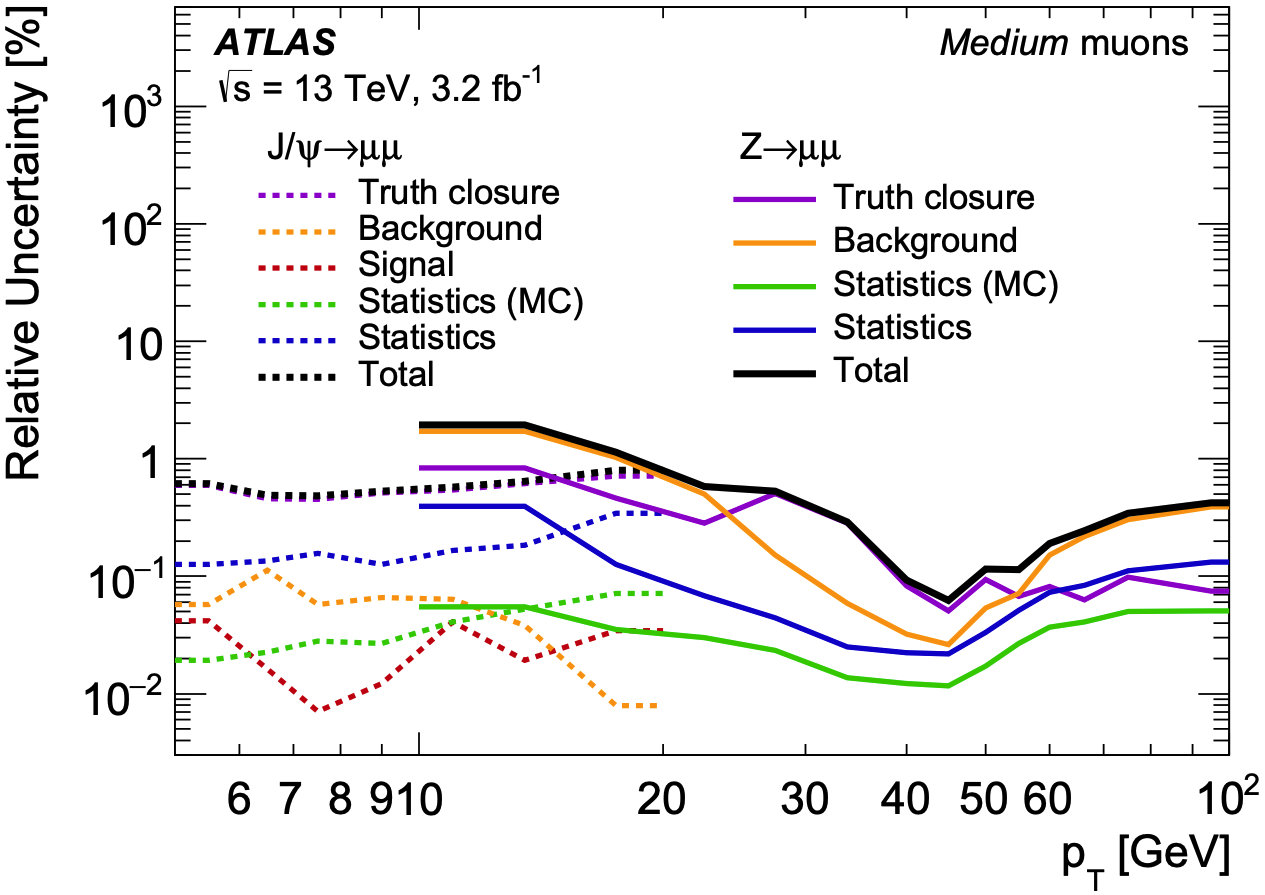
\includegraphics[width=0.8\linewidth]{figures/objects/medium_muons}
  \caption{Total uncertainty in the efficiency scale factor for Medium muons as a function of $\pT$ as measured in $Z \rightarrow \mu\mu$ (solid lines) and $J/\Psi \rightarrow \mu\mu$ (dashed lines) decays. The combined uncertainty is the sum in quadrature of the individual contributions \cite{Aad:2016jkr}.}
  \label{sec:objects:medium_muons}
\end{figure}

\section{Overlap Removal} \label{sec:objects:overlap}



\chapter{Event Selection} \label{chap:selection}

Having created our physics objects we begin to make selections of what types of
events we want to consider given the goal of our analysis.  In our boosted
topology this means considering things like momentum, jet collection efficiencies and
background rejection.

\section{Selected Triggers} \label{sec:selection:triggers}

This analysis uses exclusively large-$R$ jet triggers in order to maximally
capture the boosted decay products of the Higgs. However, pile-up increased
over the course of LHC Run 2 as shown in \Cref{fig:pileup}. This increase in
pile-up corresponds to an increase in the underlying event energy that can be
clustered into jets and thus an increase in the rate of the large-$R$ jet
trigger. As a result the High Level Trigger (HLT) $\pT$ requirement was
increased over the years in order to maintain a low trigger rate for data
recording.  This results in a different triggering algorithm for the 2015,
2016, and 2017 data taking years.  While all the triggers require a large-$R$
jet to be reconstructed in the HLT, the 2015 and 2016 triggers used an
ungroomed (a10) large-$R$ jet algorithm while in 2017 a trimmed (a10t) version
was used.  In 2015 the large-$R$ trigger looked for an ungroomed large-$R$ jet
with $\pT > 360~\GeV$.  In 2016 the $\pT$ threshold was raised to $420~\GeV$.
In 2017 the requirement changed to look for a trimmed large-$R$ jet with $\pT >
480~\GeV$.  This information is summarized in \Cref{table:triggers}, which also
details the integrated luminosity for the various triggers as well as the
offline $\pT$ threshold.  Notice that the offline threshold differs from the
HLT threshold.  This is due to the fact that the trigger must make a quick
calculation of the jet energy in order to keep data rates low. However, this
online calculation sacrifices accuracy, so some jets that should have
passed are instead ignored.  This results in a turn-on curve in the $\pT$
distribution near the online threshold where the trigger is not yet fully
efficient. Thus, a higher offline threshold is chosen corresponding to when the
trigger is fully efficient.  All triggers used in this analysis are fully
efficient for an offline threshold of $\pT > 480~\GeV$.  In order make sure the
triggers are fully efficient for our offline selection, all events are required
to contain a trimmed large-$R$ jet with $\pT > 480~\GeV$.

\begin{table}[htpb]
 \centering 
  \caption{ Summary of the large-$R$ jet triggers used for the data taking
periods of 2015, 2016, and 2017 and the offline $\pT$ thresholds at which
they become fully efficient. The recorded integrated luminosity for each
trigger is also included.}
 \begin{tabular}{@{}rlrr@{}}
  \toprule
  Year   & Trigger Name                 & Offline $\pT$ Threshold~$(\GeV)$ & Luminosity~$\left(\ifb\right)$ \\ \midrule
  $2015$ & $\text{HLT\_j360\_a10\_lcw\_sub\_L1J100}$  & $410$                              & $3.2$                          \\
  $2016$ & $\text{HLT\_j420\_a10\_lcw\_L1J100}$      & $450$                              & $33.0$                         \\
  $2017$ & $\text{HLT\_j460\_a10t\_lcw\_jes\_L1J100}$ & $480$                              & $44.3$                         \\
  \bottomrule
 \end{tabular}
 \label{table:triggers}
\end{table}

\section{Pre-selection Studies} \label{sec:selection:pre_selection}

\section{Signal Selection} \label{sec:selection:signal_selection}

\section{Optimisation} \label{sec:selection:optimisation}


\chapter{Background Estimation} \label{chap:background}

The dominant background was QCD.  I worked on the ttbar control region.  The Vqq
and single top backgrounds were estimated from monte carlo.

\section{Multijet QCD estimation} \label{sec:background:qcd}

The dominant background contribution to the SR comes from the non-resonant
multijet QCD process. Unfortunately the estimation of this process through MC
is not reliable due to the statistical precision of available samples and the
underlying inaccuracies of the event generation.  Thus, a data-driven estimate
was employed by fitting the large-$R$ jet mass distribution, $m_{J}$, in the SR
with a parametric function after validation of the procedure in the
$\text{CR}_{\text{QCD}}$.  This approach is further motivated by the good
agreement in shape of the $\text{CR}_{\text{QCD}}$ and SR over the mass range
of the fit, $70~\GeV$ to $230~\GeV$, as seen in
\Cref{fig:selection:sr_cr_shape}. A brief summary of this process is presented
below, with in-depth details available in Reference \cite{Feickert:2690521}.

The statistical precision of $\sim 1~\ifb$ of the
$\text{CR}_{\text{QCD}}$ is found to be comparable to that of the SR for a
luminosity of $80.5~\ifb$.  Thus, the $\text{CR}_{\text{QCD}}$ was
broken into 60 slices constructed using adjacent data runs resulting in an
average of $1.2~\ifb$ of data per slice.

Two families of parametric functions were used for this modeling.  The
polynomial exponential function was chosen to be the nominal model

\begin{equation}
\label{sec:background:polynomial}
f_{n} \left(x \middle|\,\vec{\theta}\right) = \theta_{0}\, \exp\left(\sum_{i=1}^{n} \theta_{i}\,x^{i}\right), \quad x = \frac{m_{J} - 150~\GeV}{80~\GeV},
\end{equation}

and the alternative model, the formal Laurent series,

\begin{equation}
\label{sec:background:laurent}
f_{n} \left(x \middle|\,\vec{\theta}\right) = a \sum_{i=0}^{n} \frac{\theta_{i}}{x^{i+1}}, \quad a=10^{5},\,x = \frac{m_{J} + 90~\GeV}{160~\GeV}.
\end{equation}

The $\theta$ coefficients are determined by the fit, $a$ is empirically chosen
to keep the scale of parameters at $\mathcal{O}(1)$, and the independent
variable $x$ parameterizes the fit range $m_{J}\in[70,230]$ GeV to $x\in[-1,1]$
for \Cref{sec:background:polynomial} and $x\in[1,2]$ for
\Cref{sec:background:laurent}.  This reparameterization was empirically seen to
provide improved numerical stability in the fit.

Both functions are tested on a random $\text{CR}_{\text{QCD}}$ slice to
determine the minimum number of model parameters needed to describe the shape
of the distribution.  The $Z$ + jets, $W$ + jets, and
$k$-factor corrected $t\bar{t}$ contributions are all scaled
by their cross sections times the luminosity and then subtracted from the slice
to remove bias from the fit.  The results of a likelihood ratio test with
Wilks' theorem \cite{wilks1938} and the $F$-test
\cite{snecdecor1991statistical} were both used to determine the minimum number
of model parameters for both function choices.  The Wilks test preferred a
five-parameter model for both while the $F$-test preferred a four-parameter
model for both.  To be conservative in our final estimate, the five-parameter
model was chosen for both the polynomial exponential function and the formal
Laurent series.

In order to determine the robustness of these fit functions, they were validated
using all of the $\text{CR}_{\text{QCD}}$ slices.  For these validation studies
the fit included properly scaled $Z$ + jets, $W$ + jets, $t\bar{t}$ and single
top contributions in addition to the $\text{CR}_{\text{QCD}}$ slice. Within the
statistical precision given by the different data slices, the $\chi^{2}/\text{ndf}$
from the individual fits is found to follow the expected distribution of a good
fit.

\section{Top Quark Pair Background} \label{sec:background:ttbar}

The substantial contribution to the SR by boosted $t\bar{t}$ production shown
in \Cref{table:efficiencies_and_yields} makes its modeling a top
priority~\footnote{Pun!}.  Unfortunately, current MC generators are not able to
predict the $t\bar{t}$ cross section well in this boosted regime as seen in
\Cref{sec:background:mismodeling}.  This long-standing issue is likely due to
missing higher-order diagrams rather than due to suboptimal generator setup
\cite{ATL-PHYS-PUB-2018-009}.  To compensate for this mismodeling the
$t\bar{t}$ yield in the SR is corrected with a normalization scale factor.  The
scale factor, or $k$-factor, is derived by fitting the $t\bar{t}$ normalization
of the in the $t\bar{t}$ enriched control region ($\text{CR}_{t\bar{t}}$).  In
the final fit the SR $t\bar{t}$ MC sample is fit by a double-sided Crystal Ball
function \cite{Gaiser:1982yw} to smooth out statistical fluctuations, and then
its normalization is constrained with the derived flat $k$-factor using its
uncertainty.

\begin{figure}[!htbp]
\centering
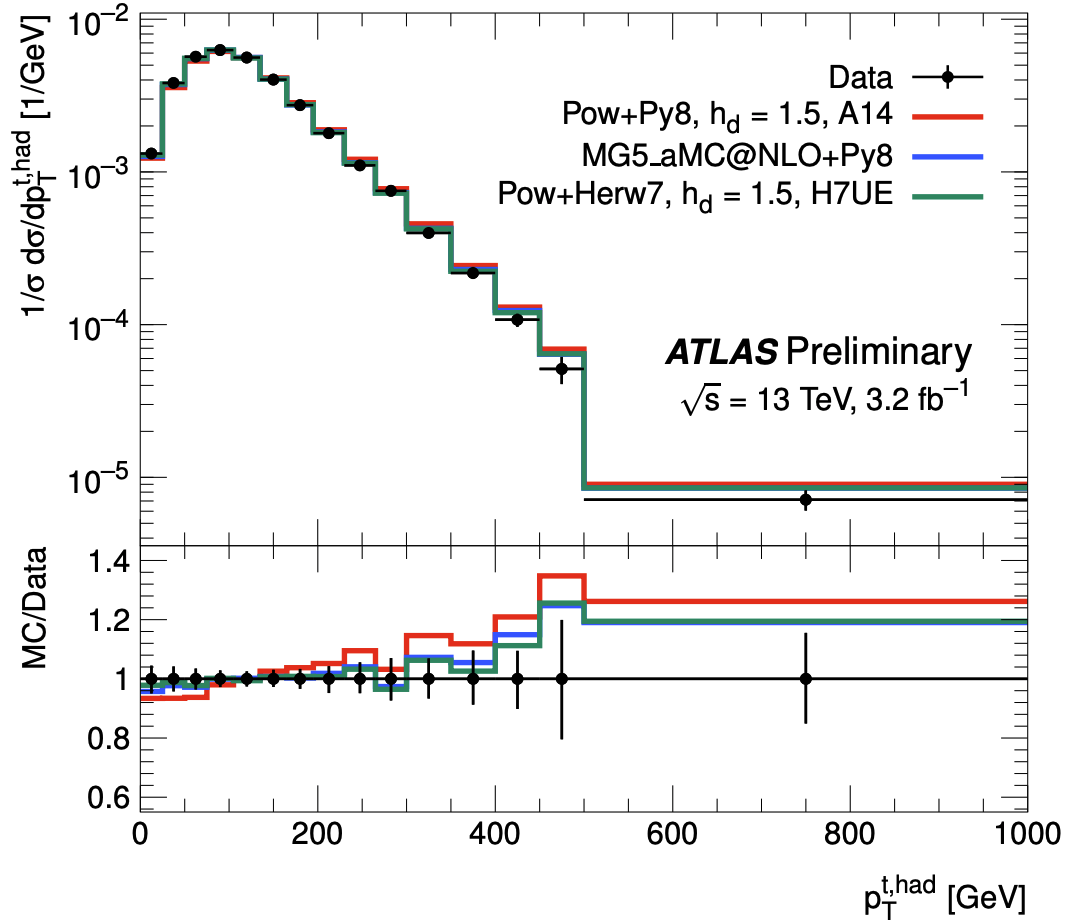
\includegraphics[width=0.6\linewidth]{figures/backgrounds/mismodeling}
\caption{Comparison in $\pT$ of the top quark for different generator setups
used to assess the NLO+PS matching as well as the parton shower and
hadronization uncertainty after optimization, compared to data at $\sqrt{s} =
13~\TeV$ \cite{ATL-PHYS-PUB-2018-009}.}
\label{sec:background:mismodeling}
\end{figure}

\subsection{Constructing the $\text{CR}_{t\bar{t}}$ Control Region}

The $t\bar{t}$-enriched control region uses the same $\pT$ selections as the
signal candidate large-$R$ jet in addition to the following criteria to select
$t\bar{t}$ events like the one shown in \Cref{sec:background:ttbar_depiction}.
Three regions are defined by requiring zero ($\text{CR}_{t\bar{t}0}$), one
($\text{CR}_{t\bar{t}}$) or two ($\text{CR}_{t\bar{t}2}$) tight quality
$b$-tags in the two leading VR track jets of the signal candidate. The
configuration with exactly one $b$-tag, $\text{CR}_{t\bar{t}}$, is was chosen
to exploit the single $b$-quark that results from the dominant decay mode of
the top quark $t \rightarrow bW$.  This one $b$-tag region has contributions from
$t\bar{t}$, single-top, $Z$ and $H$ when one $b$-tag is lost, and multijet when
the $b$-tag is faked.  The other two regions are used to validate the
extrapolation of the $k$-factor into the $\text{CR}_{\text{QCD}}$ and SR.

\begin{figure}[!htbp]
  \centering
\subcaptionbox{\label{sec:backgrounds:ttbar_feynman}}{
\resizebox{0.48\linewidth}{!}{
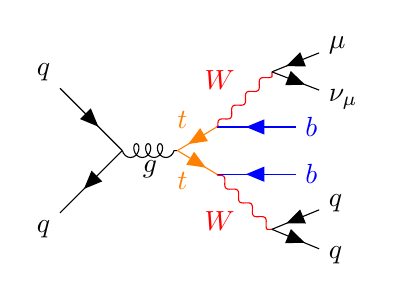
\begin{tikzpicture}
  \begin{feynman}
    % initial state particles
    \vertex (i1) {\(q\)};
    \vertex [below=2cm of i1] (i2) {\(q\)};

    % vertices
    \vertex [below right=1.cm and 1cm of i1] (a);
    \vertex [right=0.7cm of a] (b);

    % final state particles
    \vertex [above right=0.3cm and 0.5cm of b] (t1);
    \vertex [below right=0.3cm and 0.5cm of b] (t2);

    \vertex [above right=0.7cm and 0.7cm of t1] (W1);
    \vertex [blue, right=1.0cm of t1] (f1) {\(b\)};

    \vertex [blue, right=1.0cm of t2] (f2) {\(b\)};
    \vertex [below right=0.7cm and 0.7cm of t2] (W2);

    \vertex [above right=0.1cm and .6cm of W1] (f3) {\(\mu\)};
    \vertex [below right=0.1cm and .6cm of W1] (f4) {\(\nu_{\mu}\)};
    \vertex [above right=0.1cm and .6cm of W2] (f5) {\(q\)};
    \vertex [below right=0.1cm and .6cm of W2] (f6) {\(q\)};

    \diagram* {
      (i1) -- [fermion] (a) 
        -- [fermion] (i2),

      (a) -- [gluon, edge label'=\(g\)] (b),

      (t1) -- [orange, fermion, edge label'=\(t\)] (b)
        -- [orange, fermion, edge label'=\(t\)] (t2),

      (f1) -- [blue, fermion] (t1)
        -- [red, boson, edge label=\(W\)] (W1),
      (f2) -- [blue, fermion] (t2)
        -- [red, boson, edge label'=\(W\)] (W2),

      (f3) -- [fermion] (W1)
        -- [fermion] (f4),
      (f5) -- [fermion] (W2)
        -- [fermion] (f6),
    };

      
  \end{feynman}
\end{tikzpicture}
}} \hfill
\subcaptionbox{\label{sec:backgrounds:ttbar_cartoon}}{
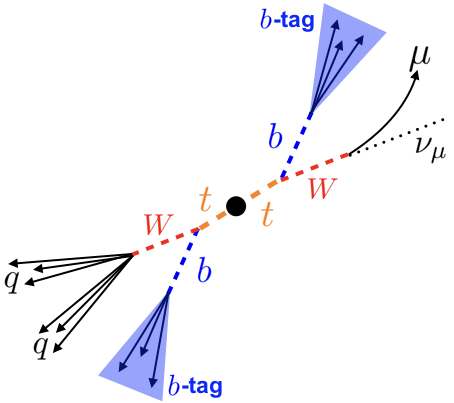
\includegraphics[width=0.48\linewidth]{figures/backgrounds/ttbar_cartoon}
}

\caption{(a) Feynman diagram of $t\bar{t}$ decay to $b$-quarks and leptonic $W$-boson decays. (b) Cartoon depicting $t\bar{t}$ decay to $b$-quarks and leptonic $W$-boson decays in center of mass frame.}
\label{sec:background:ttbar_depiction}

\end{figure}

To reduce multijet contamination in the sample the second top quark in the
opposite hemisphere of the signal candidate is required to decay leptonically
in the muon channel. \Cref{sec:backgrounds:phi_study} compares the $\Delta\phi$
between the leading muon in the event and the signal candidate jet for the
multijet and $t\bar{t}$ MC samples. This distribution shows the expected
back-to-back topology of the $t\bar{t}$ system depicted in
\Cref{sec:backgrounds:ttbar_cartoon} versus the multijet sample where the muons
come from the signal candidate due to hadron decays in flight. Thus, a cut of
$\Delta\phi(\text{muon} - \text{signal}) > \frac{2\pi}{3}$ was chosen to reduce
the QCD contribution by several orders of magnitude while only reducing the
$t\bar{t}$ contribution by roughly a factor of three~\footnote{This is expected
as the leptonic decay of $W$ is mostly agnostic to lepton flavor giving them
roughly uniform branching fractions, $BR(W \rightarrow \mu \nu_{\mu}) / BR(W
\rightarrow l \nu_l) = \frac{1}{3}$.  This is known as the universality of the
weak interaction}.

The QCD contribution is further suppressed by a cut on the muon $\pT$.
\Cref{sec:backgrounds:pt_study} compares the $\pT$ spectra for $t\bar{t}$ and
QCD before the $\Delta\phi$ cut selection. The larger mass of the $W$
boson leads to higher $\pT$ muons than the softer QCD-initiated muons.

\begin{figure}[!htbp]
\centering
\subcaptionbox{$\Delta \phi(\text{leading muon}-\text{signal})$ study \label{sec:backgrounds:phi_study}}{
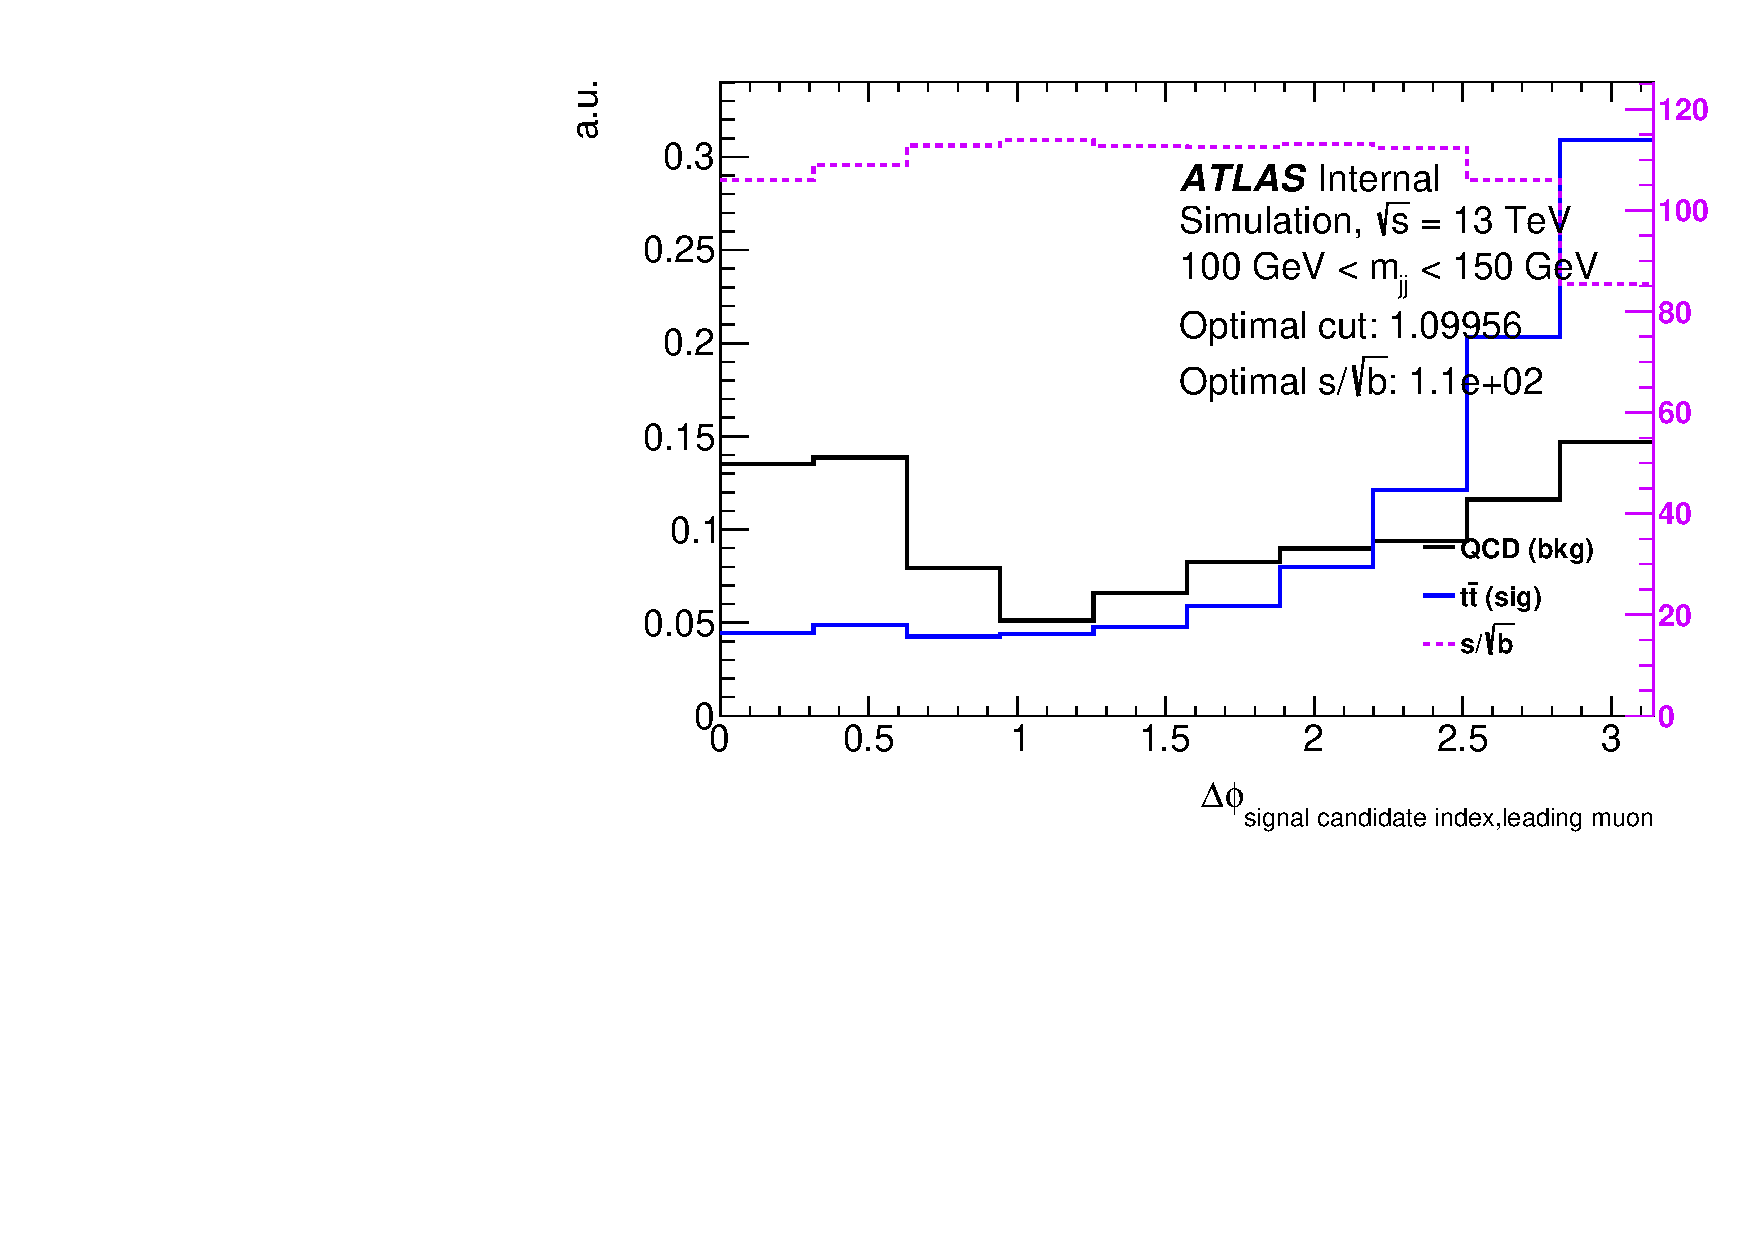
\includegraphics[width=0.48\linewidth]{figures/backgrounds/phi_study}
}\hfill
\subcaptionbox{Leading muon $\pT$ study \label{sec:backgrounds:pt_study}}{
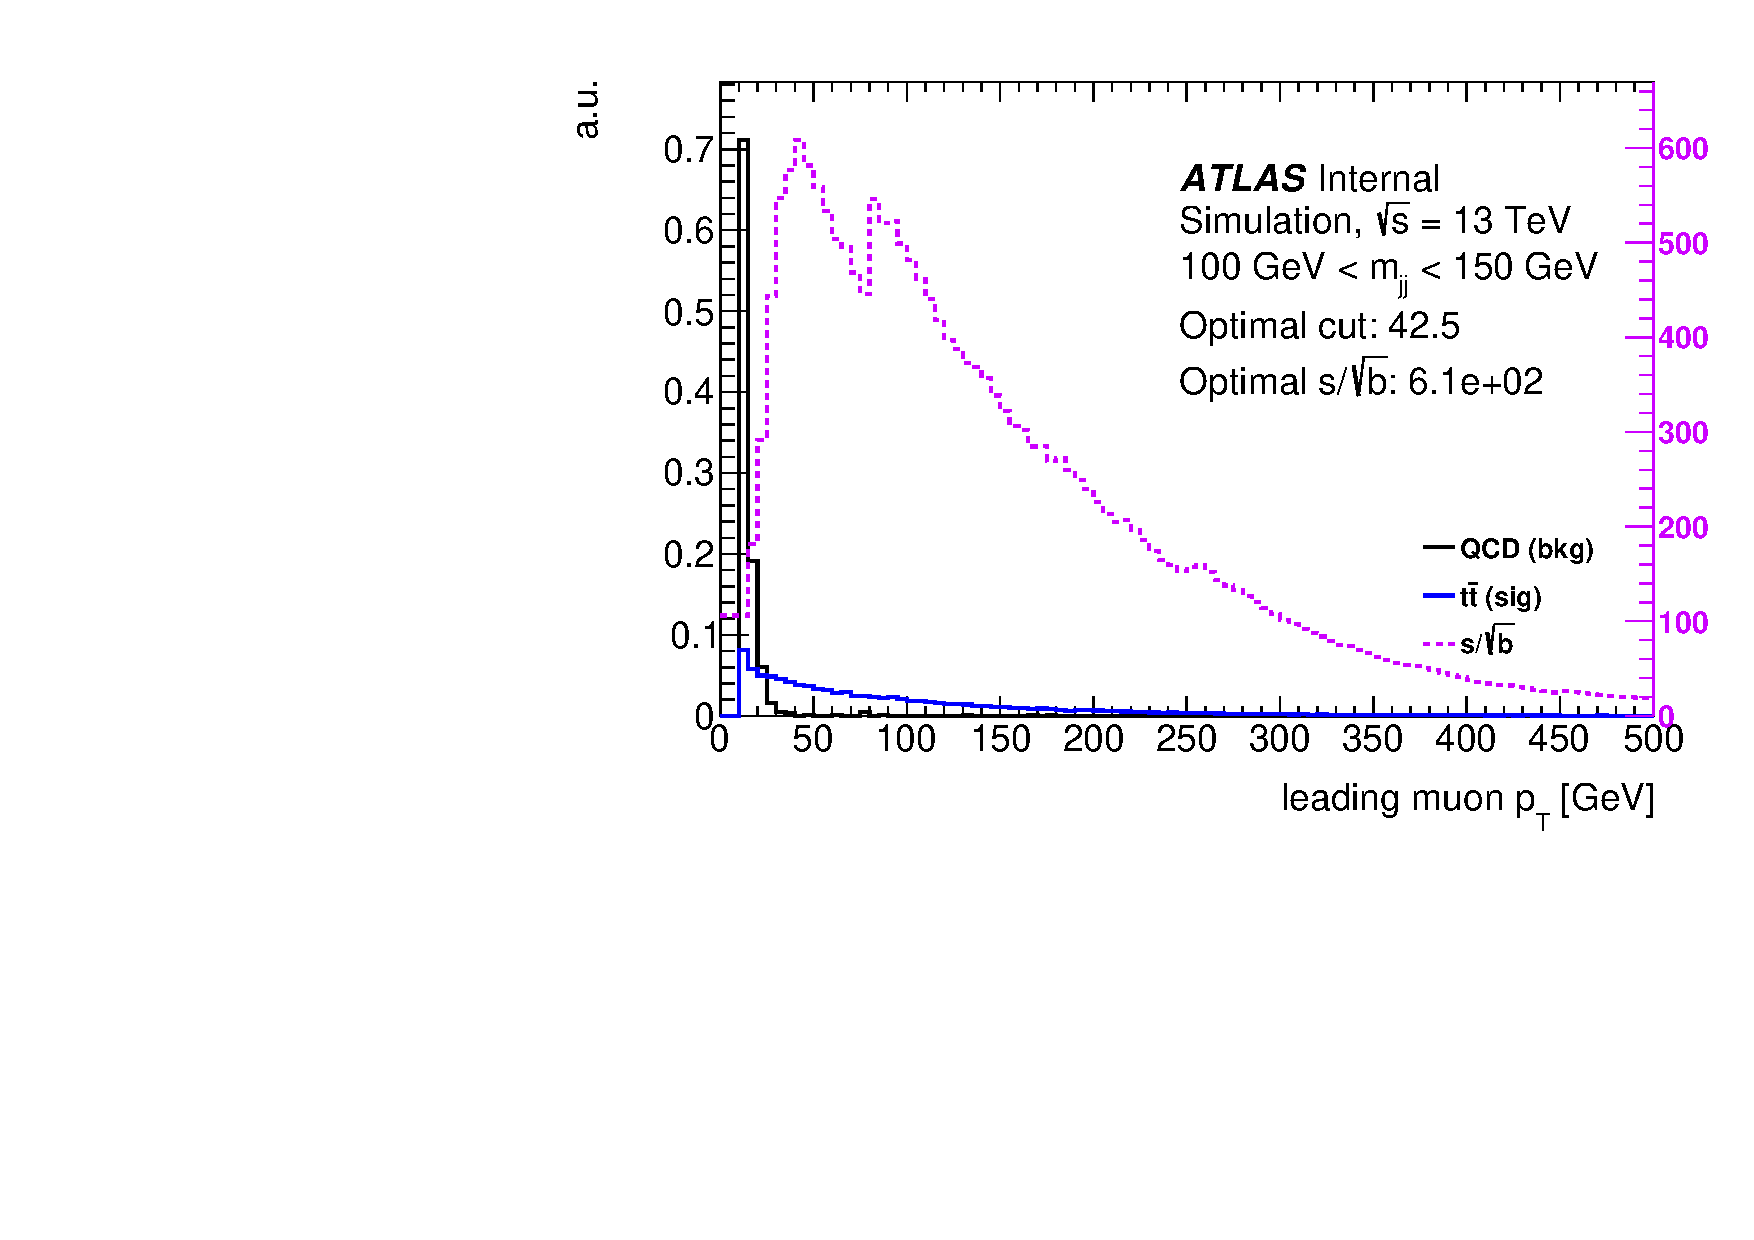
\includegraphics[width=0.48\linewidth]{figures/backgrounds/pt_study}
}
\caption{Comparison of the two variables, $\Delta \phi(\text{leading muon}-\text{signal})$ (a) and muon $\pT$ (b), between \textsc{Pythia}8 multijet and \textsc{Powheg} \ttbar simulated events used to create the \ttbar control region. The selection requires exactly one $b$-tagged track jet in the signal candidate \largeR jet. The magenta line shows the expected $s/\sqrt{b}$ significance with $80.5~\ifb$ \cite{Alison:2649017}.}
\label{sec:background:qcd_rejection_studies}
\end{figure}

Finally, at least one tight $b$-tagged track-jet is required to be within
$\Delta R < 1.5$ of the chosen muon.  This requirement exploits the collimation
of the decay products of the boosted top quark $t \rightarrow
b\mu\nu_{\mu}$.  This requirement reduces the contamination from $V(ll)$+jets
and $VV$ events. The above $\text{CR}_{t\bar{t}}$ requirements are summarized visually in \Cref{sec:background:ttbar_selection_diagram}.

\begin{figure}[!htbp]
\centering
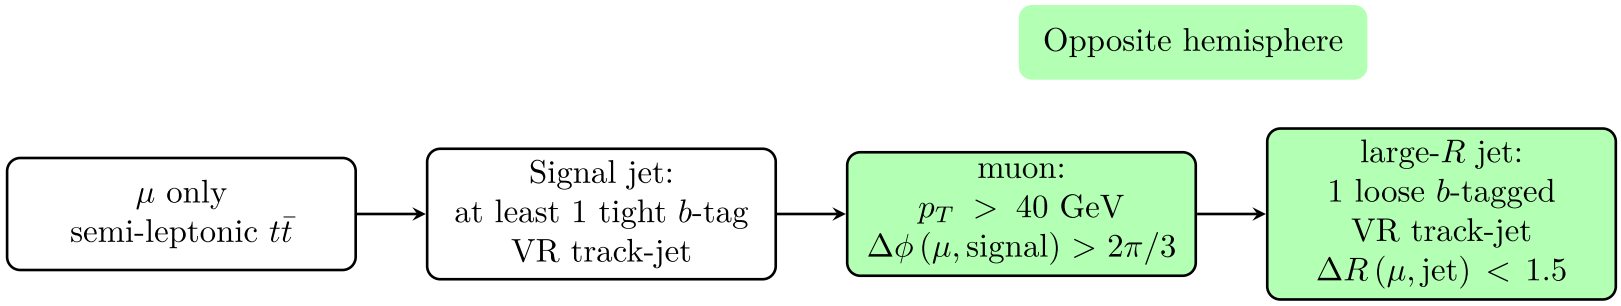
\includegraphics[width=1.0\linewidth]{figures/backgrounds/ttbar_selection}
\caption{Diagram of the $\text{CR}_{t\bar{t}}$ selection criteria \cite {Feickert:2690521}.}
\label{sec:background:ttbar_selection_diagram}
\end{figure}

\subsection{$k$-factor Estimation}

Finally the $t\bar{t}$ MC template is fit to the data in the
$\text{CR}_{t\bar{t}}$ over the mass range $100~\GeV$ to $200~\GeV$.  Single
top ($Wt$) and $W \rightarrow l\nu$ templates were included in the fit with
their normalizations kept constant. The full statistical and systematic
uncertainty is determined by running the Bayesian Analysis Toolkit (BAT)
\cite{Beaujean:2011zz}, discussed in \Cref{chap:fit}, with the large-$R$ jet
energy scale (JES), jet mass resolution (JMR), luminosity, $t\bar{t}$
modeling and flavor tagging systematic uncertainties discussed in
\Cref{chap:systematics}.

The pre- and post-fit distributions for the $\text{CR}_{t\bar{t}}$ are shown in
\Cref{sec:background:ttbar_fit} with the pull distributions shown in
\Cref{sec:background:ttbar_pulls}.  The JES and JMR systematics are constrained
by information about the peak in $t\bar{t}$ which was not available in the
dataset used to derive the recommendations. A $k$-factor of $0.84 \pm 0.11$ is
found for $\text{CR}_{t\bar{t}}$, showing that the MC overestimates the
$t\bar{t}$ yield as expected (see \Cref{sec:background:mismodeling}). This
value is used to constrain the $t\bar{t}$ contribution in the final fit to the
SR. The results for all three $t\bar{t}$ control regions are given in
\Cref{table:ttbar_kfactors}.  All three regions are consistent with eachoother
and the results of the dedicated boosted top quark study presented in reference
\cite{ATLAS:2016jct}.

\begin{table}
  \centering
  \caption{The \ttbar scale factors and their uncertainties from the three \ttbar
control regions. The value for CRttbar is used in the Signal Region. NOTE:
CRttbar2 fit failed due to low statistics but is almostly completely dominated
by ttbar in this region.  The value here is the simple ratio of number of events in ttbar
vs. data, and the uncertainty is the $t\bar{t}$ statistical uncertainty.}
  \begin{tabular}{@{}lrr@{}}
    \toprule
    Region & scale factor & uncertainty \\
    \midrule
    CRttbar0 & $0.87$ & $0.12$ \\
    CRttbar  & $0.84$ & $0.11$ \\
    CRttbar2 & $0.96$ & $0.21$ \\
    \bottomrule
  \end{tabular}
  \label{table:ttbar_kfactors}
\end{table}

\begin{figure}[!htbp]
\centering
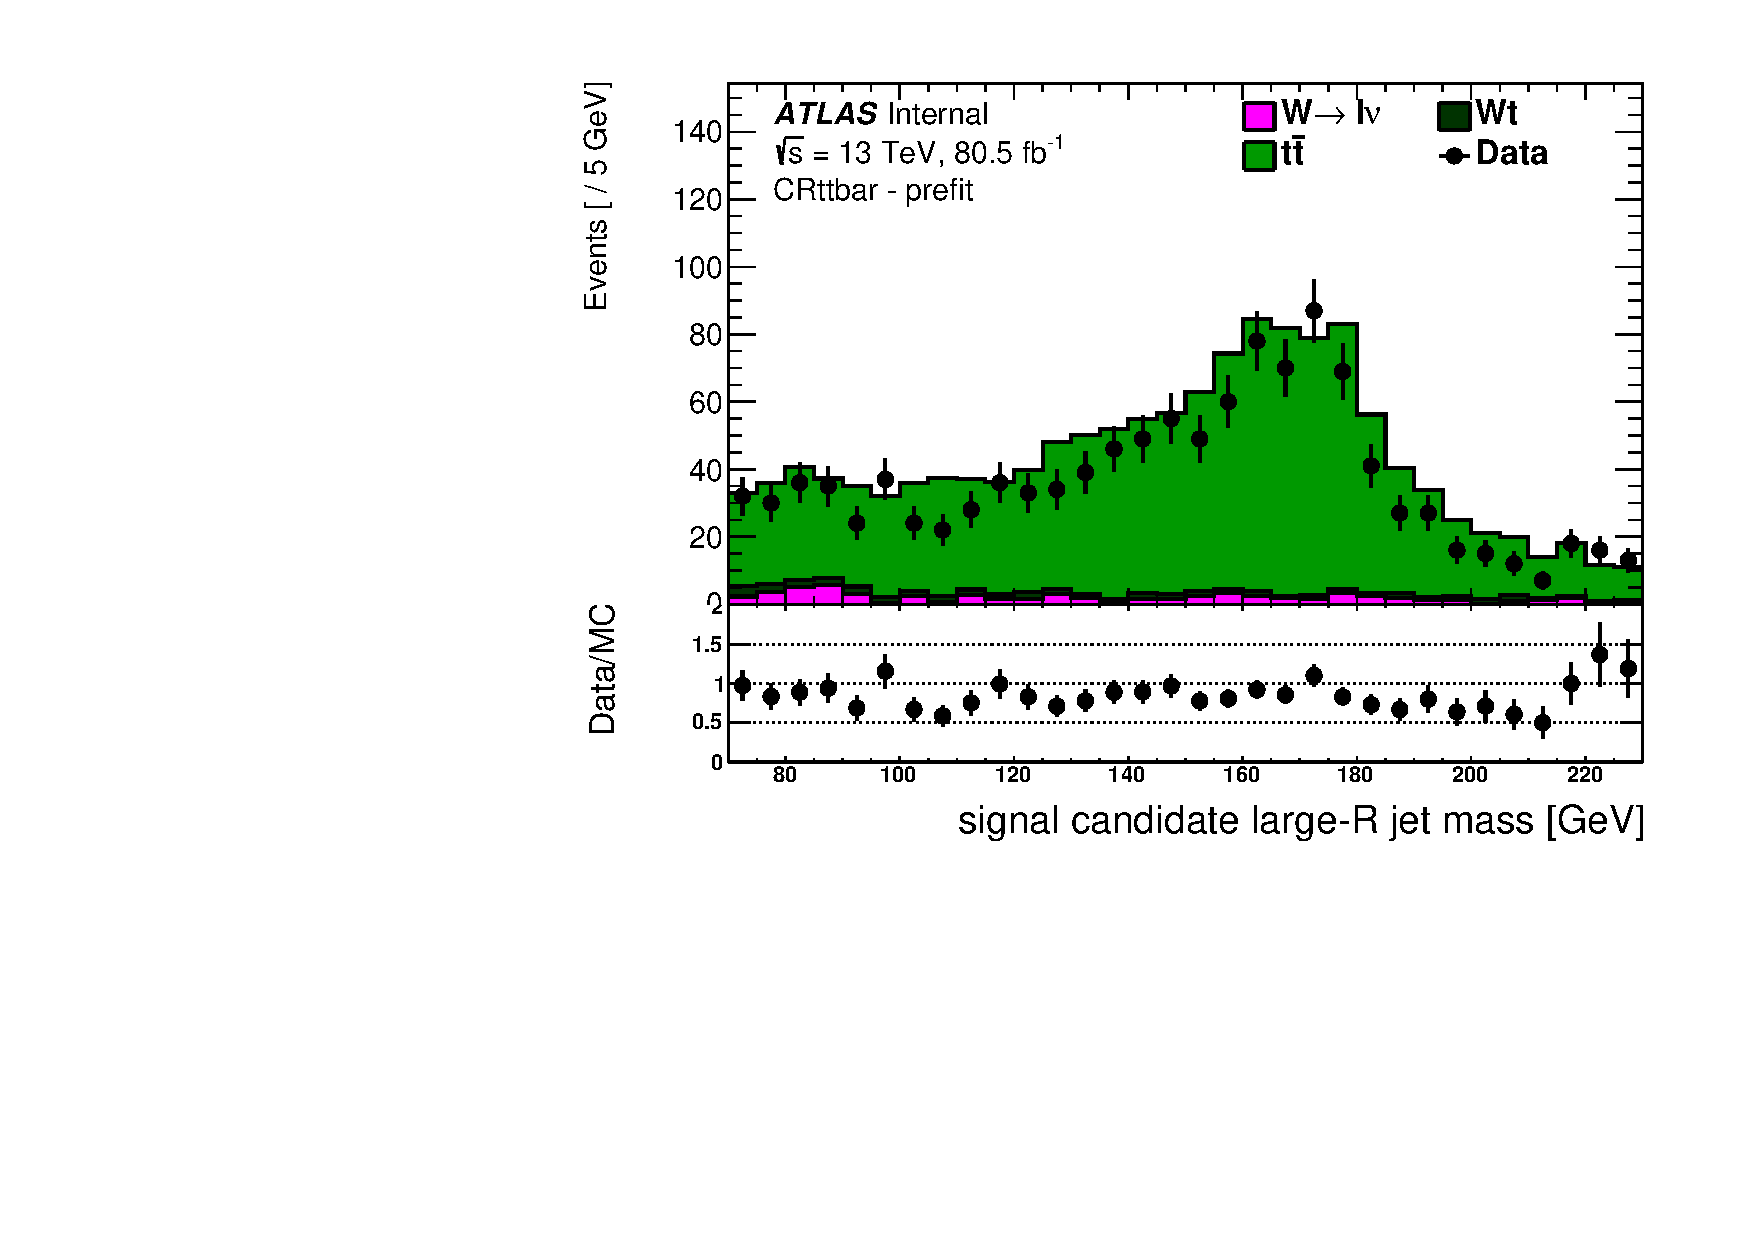
\includegraphics[width=0.49\linewidth]{figures/backgrounds/ttbar_prefit} \hfill
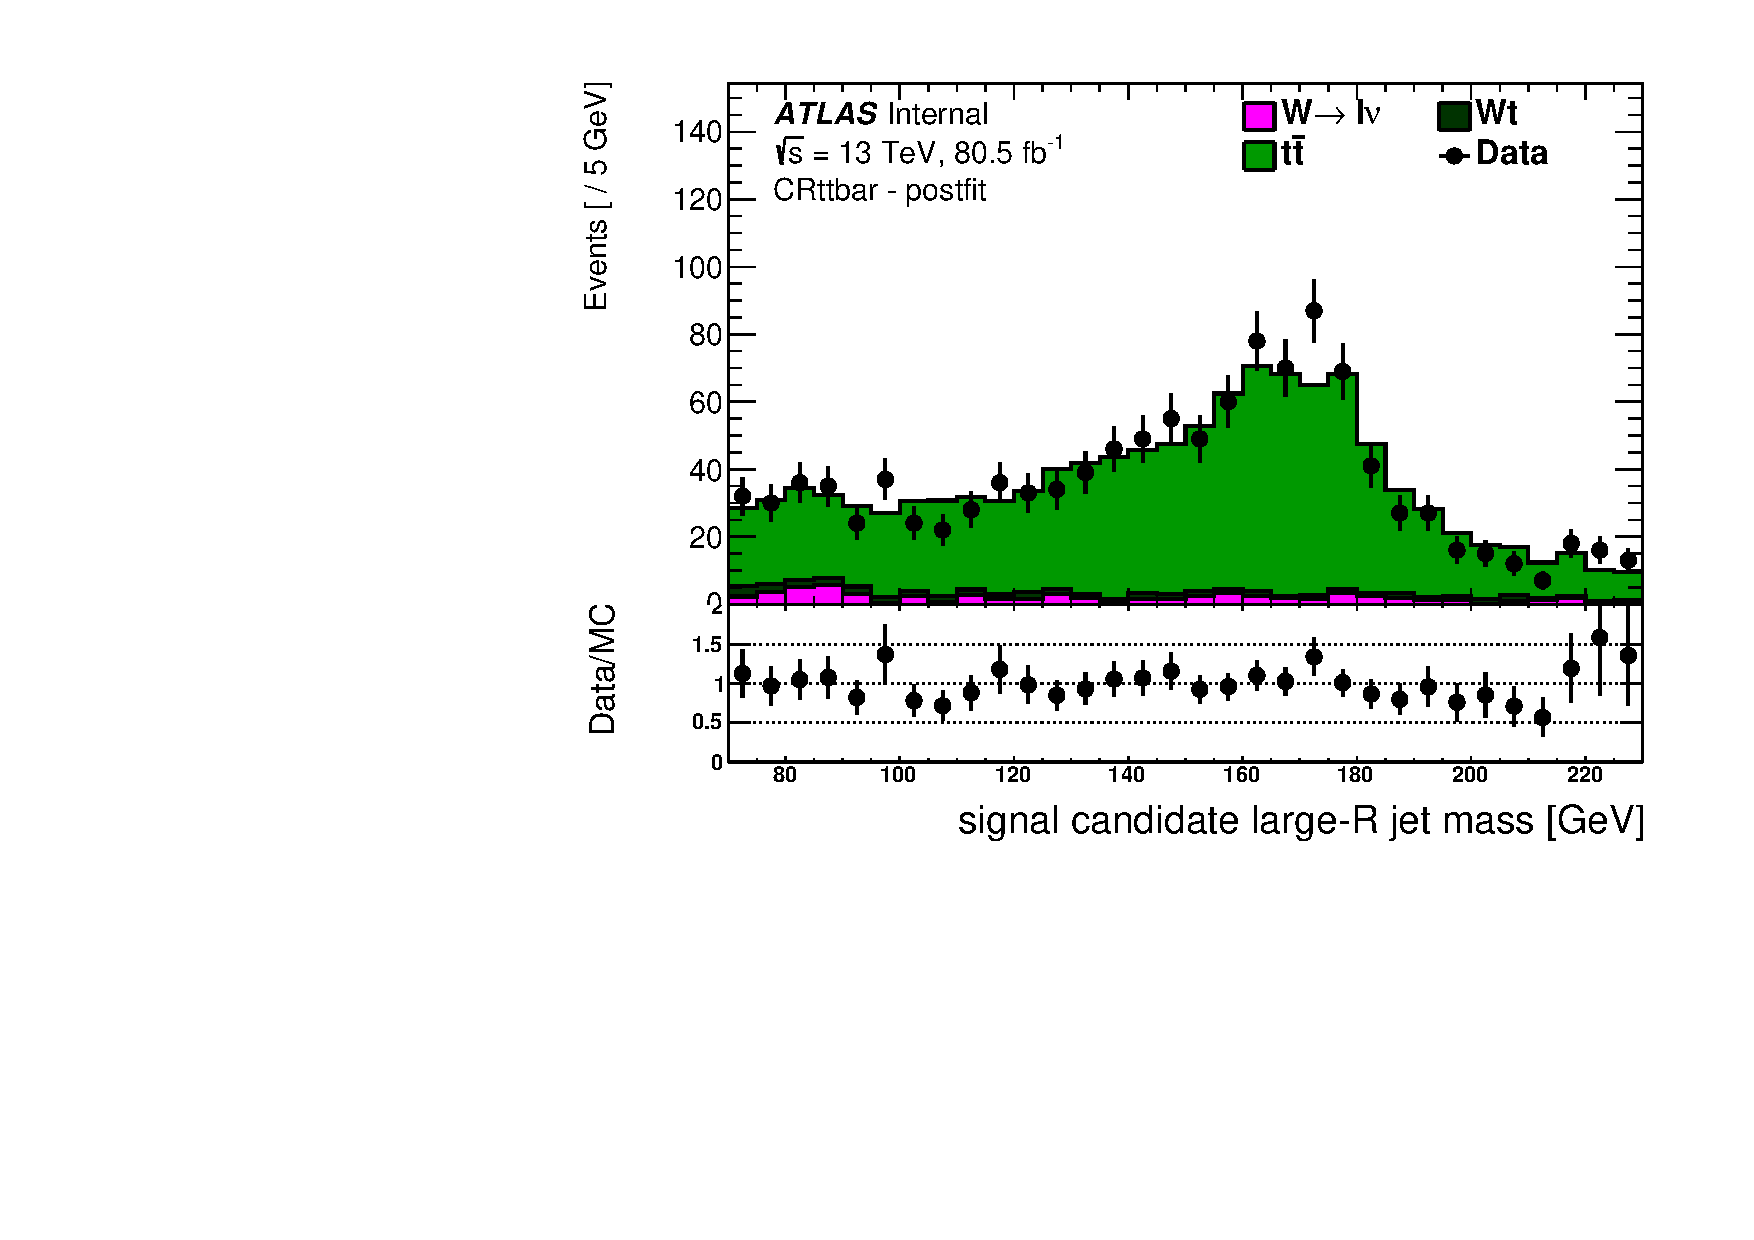
\includegraphics[width=0.49\linewidth]{figures/backgrounds/ttbar_postfit}
\caption{The pre-fit (left) and post-fit (right) data vs MC comparison for fitting the $\text{CR}_{t\bar{t}}$ region.}
\label{sec:background:ttbar_fit}
\end{figure}

\begin{figure}[!htbp]
\centering
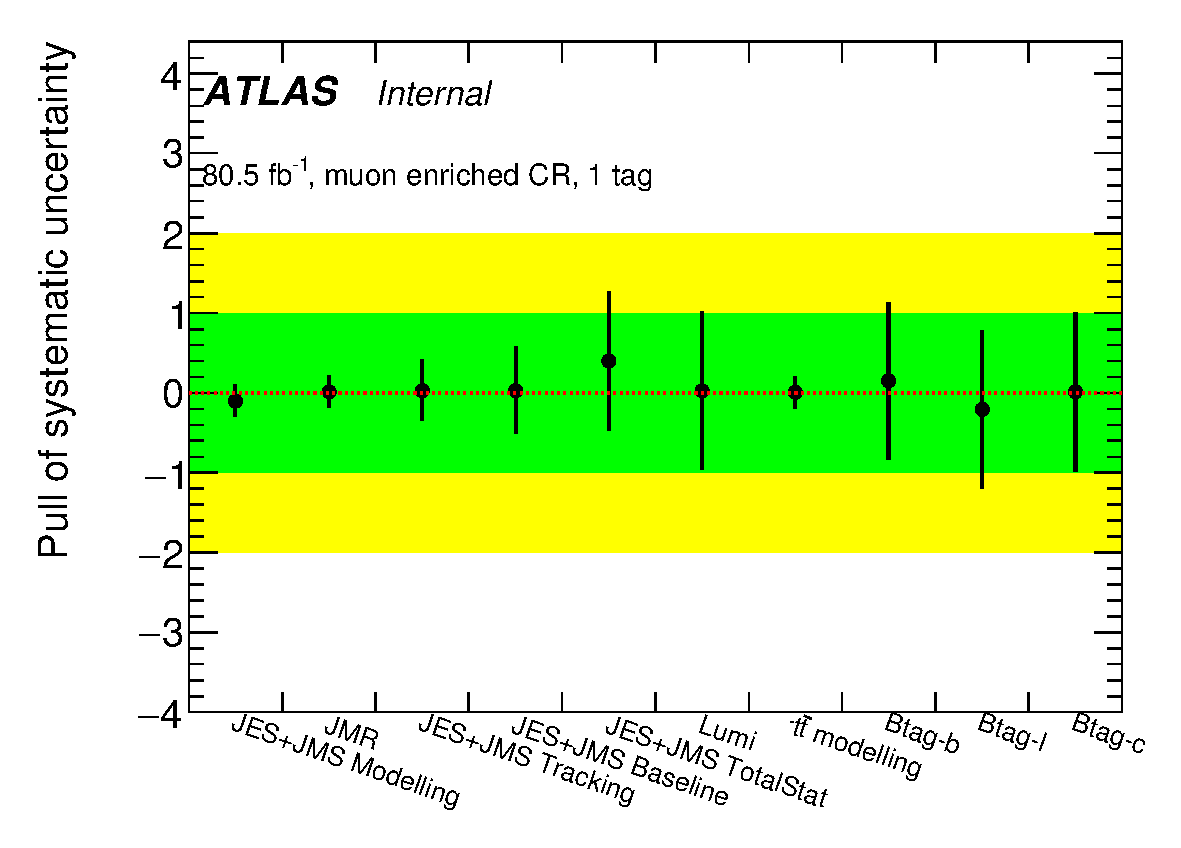
\includegraphics[width=0.7\linewidth]{figures/backgrounds/ttbar_pulls}
\caption{The pull distributions for the different nuisance parameters used in the $\text{CR}_{t\bar{t}}$ fit.}
\label{sec:background:ttbar_pulls}
\end{figure}

\section{Single top estimation} \label{sec:background:single_top}

\section{Hadronic Vector Boson Background} \label{sec:background:vqq}

The $V+\text{jets}$ template is constructed by fitting the generated MC
histogram with the sum of three Gaussians plus a constant term.  The systematic
variations, discussed in \Cref{chap:systematics}, of this template are re-fit
using the same functional choices.  This results in smooth histograms to be
used as input to the fit discussed in \Cref{chap:fit}.


\chapter{Systematic Uncertainties} \label{chap:systematics}

This chapter presents the sources of systematic uncertainty in
the analysis that could result in biases to the final fit.  These sources of
uncertainty can come from experimental calibrations or procedures and from the
MC modeling of signal and background. They can contribute to uncertainties in
the overall yield (``normalization") and to the differential shape of the
signal candidate mass observable used in the statistical procedure for the
final fit.  The sources of uncertainty on the derivation of the QCD multijet
background are separated from the uncertainties on the resonant backgrounds as
the former is estimated using data while the later are estimated using MC
simulation.  Each of the relevant sources of uncertainty are briefly discussed
and a summary is presented.

\section{Uncertainties on Data-Driven QCD Modeling} \label{sec:systematics:qcd_modeling}

The QCD background estimate discussed in \Cref{sec:background:qcd} is based on
a direct fit to data. The choice of function used to fit the QCD background is
empirically based so it is important to consider the uncertainty introduced by
this choice.  This is modeled by considering the differences between the
nominal polynomial exponential function in \Cref{sec:background:polynomial} and
the alternate Formal Laurent series \Cref{sec:background:laurent} in a series
of pseudoexperiments.  To do this Poisson toys are sampled from the QCD
component of the fit to the SR which contains all components of the full model
(QCD, $Z$ + jets, $W$ + jets, $t\bar{t}$, and the Higgs boson signal) but no
nuisance parameters. The toys are then fit with the nominal and alternative
function choices.  The uncertainty bands from these two sets of fits provide a
measure of of the statistical uncertainty on the multijet parameterization
derived from the spread of fit parameters, and a systematic uncertainty on the
choice of fitting function derived from the difference between the two fitted
shapes.

\section{Uncertanties on Resonant Backgrounds and Signal} \label{sec:systematics:resonant_modeling}

All MC templates in this analysis contain uncertainties derived from the
large-$R$ jet energy and mass calibrations \cite{Aaboud:2018kfi} and the
calibration of the \texttt{MV2c10} $b$-tagging algorithm \cite{Aaboud:2018xwy}
which effects $b$, $c$, and $l$ jet flavors differently.  The jet energy and
jet mass calibration uncertanties affect both normalization and shape of the
templates.  This means their impact on the analysis must be determined by
varying the jet energy and jet mass up and down within their uncertanties and
propogating the varied templates through the entire analysis procedure.  The
effect of the jet energy resolution uncertainty was also tested, but found to
be negligible. The impacts of uncertainties on the calibration of the
\texttt{MV2c10} algorithm have been found to be independent of the large-$R$
jet mass for all MC templats and thus only affect the signal normalization.

To account for the modeling uncertanties associated with the choice of MC
generator, additional shape uncertanties are applied to the $V$ + jets and
$t\bar{t}$ templates.  The systematic is determined by taking the difference
between the large-$R$ jet mass shapes from two different MC generators.  For
$V$ + jets the nominal shape was generated using \textsc{Sherpa} 2.1.1 and then
compared to the alternate shape generated with \textsc{Herwig}++ 2.7.  For
$t\bar{t}$ the nominal shape was generated with \textsc{Powheg-Box} 2 and
compared with the alternate shape generated with \textsc{Sherpa} 2.1.1.

The $t\bar{t}$ normalization in the SR is constrained by the $k$-factor derived
from a fit to data in the $\text{CR}_{t\bar{t}}$ as discussed in
\Cref{sec:background:ttbar}.  The uncertainty on the measurement was found to
be $13\%$ and is treated as a systematic uncertainty on the $t\bar{t}$
normalization.

In order to have an accurate simulation the normalization of all MC templates
must be scaled by the integrated luminosity of the dataset in question.  The
systematic uncertainty on the integrated luminosity measurement is derived
following the methodology presented in Reference \cite{Aad:2013ucp}.  For this
analysis it was found to be $2.1\%$.

Theoretical systematic uncertanties on the normalization of the $V$ + jets and
Higgs components are added to the fit in the SR.  Theory uncertainties on the
$V$ + jets processes result from the impact of higher order electroweak and QCD
corrections to their differential cross sections \cite{Lindert:2017olm}. For
Higgs production the dominant theoretical uncertainty is from ggF production
which is taken to be $30\%$.  This is consistent with the cross section
uncertainty calculated with the MiNLO procedure and includes the effects of the
non-zero top-mass for Higgs bosons with $\pT > 400~\GeV$.  This same
uncertainty is applied for the other production mechanisms for Higgs' with
$\pT > 400~\GeV$.  The result is a total theory uncertainty on the Higgs
cross section of $30\%$.

\section{Summary of Systematics} \label{sec:systematics:summary}

The signal strength ($\mu_{s}$) is defined as the scale factor which multiplies
the cross section times branching fraction that is predicted by the signal
hypothesis being considered.  Thus, the final fit, discussed in
\Cref{chap:fit}, of our theory based MC to the SR data provides a direct
measurement of this signal strength and therefore a direct measurement of the
model's prediction. However, to understand the significance and error on this
result the statistical and systematic uncertainties must be taken into account
during the fitting procedure.

To get a sense of the the individual impact of each systematic on the total
uncertainty for the measurement of $\mu_{s}$, the following ad hoc comparison
is made.  First, the total uncertainty on $\mu_{s}$ ($\sigma_{tot}$) is
determined by running the fit with all sources of error (systematic and
statistical) allowed to float within their defined constraints.  By definition:

$$ \sigma_{\text{tot}}^{2} \; = {\underbrace{\sum_{i}^{n} \sigma_{i}^{2}}_{\substack{\text{Contributions from} \\ \text{n systematics}}}} + {\underbrace{\vphantom{\sum_{i}^{n}} \sigma_{\text{stat.}}}_{\substack{\text{Contribution from} \\ \text{statistics}}}}$$

Next, the fit is re-run with all systematics fixed to their pre-fit values
except for the systematic being investigated for its impact. This gives us
$\sigma_{i}$, the uncertainty on $\mu_{s}$ when only considering the effect of
the $i^{th}$ nuisance parameter. Note that the statistical uncertainty
($\sigma_{\text{stat}}$) is still included as it is inherent to the fitting
procedure.

Finally we take the difference in quadrature between $\sigma_{\text{tot}}$ and
$\sigma_{i}$ and divide it by the measured $\mu_{s}$ value found in the final
fit which includes all sources of uncertainty. 

$$ \frac{\sqrt{\Delta \sigma_i^2}}{\mu_{s}} $$

This ad hoc comparison represents the impact of the $i^{th}$ nuisance parameter
on the total uncertainty of the measurement of $\mu_{s}$. A summary of the
impact of each systematic for the two considered signal models (Higgs + jets
and $V$ + jets) is presented in \Cref{table:systematic_uncertainties}

\begin{table}[htpb]
 \centering
 \caption{
  Summary of the impact $(\sqrt{\Delta \sigma_i^2}/\mu_{s})$ of the main systematic uncertainties on the total uncertainty, $\sigma_{tot}$, of the measured signal strength, $\mu_{s}$, for the $V$ + jets and Higgs boson + jets signals signals~\cite{ATLAS-CONF-2018-052}.}
 \begin{adjustbox}{max width=\textwidth}
  \begin{tabular}{@{}llrrrr@{}}
   \toprule
   Source                    & Type           & $V$ + jets & Higgs + jets  \\ \midrule
   Jet energy and mass scale & Norm. \& Shape & $15\%$     & $14\%$ \\
   Jet mass resolution       & Norm. \& Shape & $20\%$     & $17\%$ \\
   $V$ + jets modeling       & Shape          & $9\%$      & $4\%$  \\
   $t\bar{t}$ modeling       & Shape          & $<1\%$     & $1\%$  \\
   $b$-tagging $(b)$         & Normalization  & $11\%$     & $12\%$ \\
   $b$-tagging $(c)$         & Normalization  & $3\%$      & $1\%$  \\
   $b$-tagging $(l)$         & Normalization  & $4\%$      & $1\%$  \\
   $t\bar{t}$ $k$-factor     & Normalization  & $2\%$      & $3\%$  \\
   Luminosity                & Normalization  & $2\%$      & $2\%$  \\
   Alternate QCD function    & Norm. \& Shape & $4\%$      & $4\%$  \\
   $W$/$Z$ and QCD (Theory)  & Normalization  & $14\%$     &        \\
   Higgs (Theory)            & Normalization  &            & $30\%$ \\
   \bottomrule
  \end{tabular}
 \end{adjustbox}
 \label{table:systematic_uncertainties}
\end{table}


\chapter{Statistical Fit} \label{chap:fit}



\section{Limit Setting and Bayes' Theorem} \label{sec:fit:theory}

\section{Implementation of Priors} \label{sec:fit:priors}

As discussed in \Cref{sec:fit:theory} the priors representing the nuisance
parameters and the signal normalization are chosen to represent the analyzer's
knowledge before the data is considered. Generally speaking, the shape of the
prior distribution for systematic uncertainties is chosen to give decreased
probability as the fit tries to pull the value away from their nominal value,
while for the signal parameter the choice is made to have as little influence
on the marginalized posterior as possible.

For the $t\bar{t}$ signal strength a Gaussian prior is used with the mean and
width determined by the fit to data in the $\text{CR}_{t\bar{t}}$.  The
Gaussian prior is then normalized to unity and defined over the range [$-\nu_{5
\cdot t\bar{t}}, \nu_{5 \cdot t\bar{t}}$], where $\nu_{5 \cdot t\bar{t}}$ is five
times the expected value for $t\bar{t}$, and is set to zero elsewhere.

The remaining nuisance parameters are included using a Gaussian prior for each
source.  The Gaussian for the QCD fit function choice uncertainty is defined in
the range [$0\sigma, 1\sigma$], where $0\sigma$ corresponds to the nominal fit
function and $1\sigma$ corresponds to the alternate fit function.  All other
sources of systematic uncertainty are defined using a Gaussian over the large
range $[-3\sigma, 3\sigma]$ to allow ample room for fluctuations.
 
The two signal models, $V$ + jets and Higgs + jets, are each included in the
combined fit by utilizing a uniform prior to represent the parameter corresponding
to the number of events.  This is done to remove analyzer bias, thus allowing
the final result to more accurately reflect the data.  Furthermore, both priors
are normalized to unity over their respective ranges for reasons discussed in
\Cref{sec:fit:bat}. The $V$ + jets uniform prior is defined to be $1/(2 \cdot
\nu_{5 \cdot V})$ over the range [$-\nu_{5 \cdot V}, \nu_{5 \cdot V}$] and zero
everywhere else. Here $\nu_{5 \cdot V}$ is defined to be five times the expected
value for $V$ + jets. The Higgs + jets uniform prior is defined to be
$1/\nu_{H\text{max}}$ over the range [$0,\nu_{H\text{max}}$] and zero elsewhere.  This
$\nu_{H\text{max}}$ is the number of Higgs + jets events corresponding to the point
where the likelihood is a factor of $10^{5}$ times smaller than its maximum
value.  In both cases the ranges were chosen to be very large so as to not
influence the result.

\section{Bayesian Analysis Toolkit} \label{sec:fit:bat}

The Bayesian Analysis Toolkit (BAT) \cite{Beaujean:2011zz,Beresford:2642397} is
used to obtain the marginalized posterior distribution \Cref{eq:fit:bayes}
discussed in \Cref{sec:fit:theory}.  It takes as input the data, the parameters
$\nu$ and $\boldsymbol{\theta}$ along with their corresponding prior
distributions discussed in \Cref{sec:fit:priors}, and the chosen likelihood
function $\mathcal{L}(\nu,\boldsymbol{\theta}|Data)$.  Here the likelihood
function is given by the product of the Poisson probability in each bin: 

\begin{equation} \label{sec:fit:likelihood}
\mathcal{L}(\nu,\boldsymbol{\theta}|Data) = \prod_{i=1}^{N} \frac{(s_{i}(\nu,\boldsymbol{\theta}) + b_{i}(\nu,\boldsymbol{\theta}))^{n_{i}}}{n_{i}!} e^{-(s_{i}(\nu,\boldsymbol{\theta}) + b_{i}(\nu,\boldsymbol{\theta}))}
\end{equation}

In the above the product runs over all N bins in the histogram being fit,
$s_{i}$ and $b_{i}$ are the expected number of signal and background events
expected in bin $i$ dependant upon $\nu$ and $\boldsymbol{\theta}$, and $n_{i}$
is the number of data events in bin $i$.  Note that in \Cref{sec:fit:priors}
the signal parameter priors are normalized to unity such that $\nu$ corresponds
to the number of signal events. Now \Cref{sec:fit:likelihood} can be used to
calculate the probability of a given set of parameter values $\nu$ and
$\boldsymbol{\theta}$ given the data.  Plugging this definition into
\Cref{eq:fit:bayes} gives us the final form of Bayes' equation used to
calculate the marginalized posterior $p(\nu|\text{Data})$ given below.

\begin{equation} \label{sec:fit:full_bayes}
p(\nu|\text{Data}) \propto \pi(\nu) \int \prod_{i=1}^{N} \frac{(s_{i}(\nu,\boldsymbol{\theta}) + b_{i}(\nu,\boldsymbol{\theta}))^{n_{i}}}{n_{i}!} e^{-(s_{i}(\nu,\boldsymbol{\theta}) + b_{i}(\nu,\boldsymbol{\theta}))} \prod_{j}\pi(\theta_j)\text{d}\boldsymbol{\theta}
\end{equation}

The final step is to calculate the integral in \Cref{sec:fit:full_bayes} across
the multi-dimentional space of $(\nu,\boldsymbol{\theta})$. However, calculating the
integral for such a large space is not computationally feasible so BAT instead
employed a Markov Chain Monte Carlo (MCMC) \cite{Betancourt2017ACI,
Beresford:2642397} in order to sammple the space efficiently.

The basic idea of a MCMC is to perform a random walk in the parameter space
$(\nu,\boldsymbol{\theta})$ making sure to spend more time sampling regions of
high probability, i.ee sampling proportional to the posterior.  The sequence of
parameter values on the walk depends only on the previous set making the
resuling dequence of parameter values a Markov Chain \cite{Markov2006}.  The
Metropolis-Hastings algorithm \cite{10.2307/2334940,Beresford:2642397} is used
to generate the Markov Chains used in BAT.  This procedure is detailed below
and an illustration of the process for only two parameters $\theta_{1}$ and
$\theta_{2}$ is shown in \Cref{sec:fit:markov_chain}.

\begin{enumerate}
\item The chain begins at position $\boldsymbol{x_{1}}$ in the parameter space to be sampled.
\item The next position, $\boldsymbol{x_{2}}$, is proposed by selecting each new parameter from a Breit-Wigner distribution centered on the value of the corresponding parameter for the current position $\boldsymbol{x_{1}}$.
\item A random number $r$ between 0 and 1 is selected from a uniform distribution.
\item The value of the posterior $p(\nu,\boldsymbol{\theta}|\text{Data})$, given in \Cref{eq:fit:posterior}, is calculated for both  $\boldsymbol{x_{1}}$ and  $\boldsymbol{x_{2}}$ resulting in $p(\nu,\boldsymbol{\theta}|\text{Data})_{1}$ and $p(\nu,\boldsymbol{\theta}|\text{Data})_{2}$.
\item If $r < \frac{p(\nu,\boldsymbol{\theta}|\text{Data})_{2}}{p(\nu,\boldsymbol{\theta}|\text{Data})_{1}}$, the algorithm transitions to the new position $\boldsymbol{x_{2}}$ and it is added to the chain. Otherwise the algorithm remains at $\boldsymbol{x_{1}}$ and it is added to the chain.
\item This process is then repeated starting from the chosen position defined as position $\boldsymbol{x_{1}}$.
\end{enumerate}

\begin{figure}[!htbp]
\centering
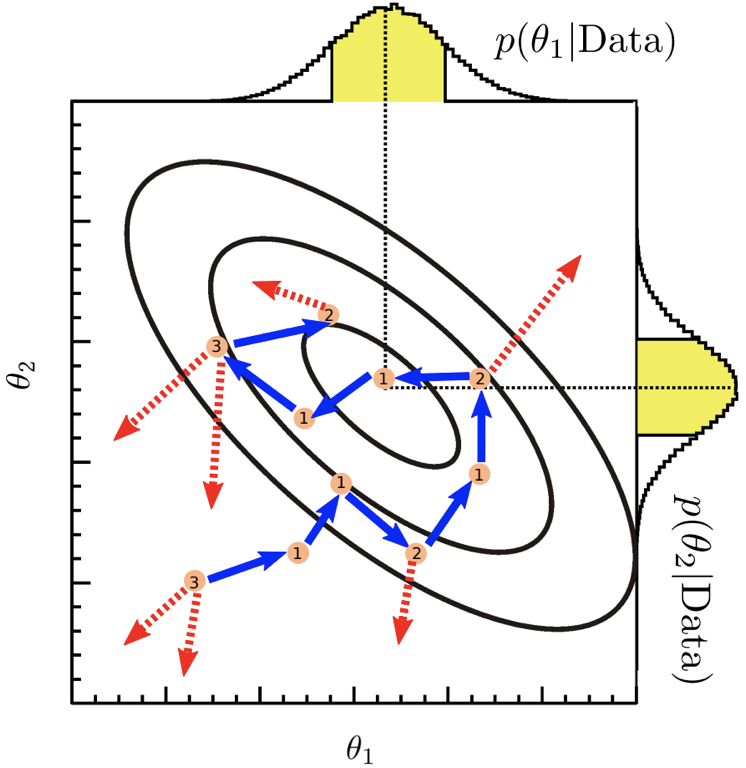
\includegraphics[width=0.7\linewidth]{figures/fit/markov_chain}
\caption{\cite{Beresford:2642397}This figure illustrates a random walk in parameter space $(\theta_{1},\theta{2})$. The numbers indicate the number of iterations the chain remained at this point in parameter space, the blue arrows indicate accepted transitions, and the red arrows indicate rejected transitions. The marginalised posterior distributions obtained for the two parameters $p(\theta_{1}|Data)$ and $p(\theta_{2}|Data)$ are also shown, and the yellow bands correspond to the central 68\% of the distributions.}
\label{sec:fit:markov_chain}
\end{figure}

This random walk in parameter space generates a chain which preferentially
transitions to positions corresponding to high probability regions of the
posterior, effectively sampling the important regions of the posterior
distribution.  By plotting the frequency of occurrence for each parameter along
the chain, and then normalizing the distribution to unity, the desired
marginalized posterior for the signal parameter $p(\nu|\text{Data})$ is found.
In \Cref{chap:results} this marginalized posterior is used to find the final
results of the analysis presented.


\chapter{Results} \label{chap:results}

This chapter summarizes the results and interpretation of the boosted $H
\rightarrow b\bar{b}$ search described in this dissertation and published in
Reference \cite{ATLAS-CONF-2018-052}.  To arrive at this point; the theory was
presented (\Cref{chap:standard_model,chap:higgs}), the data were collected
(\Cref{chap:lhc,chap:atlas}), a simulation of the data from theory was
constructed (\Cref{chap:data}), physics objects were built in data and MC
(\Cref{chap:objects}), events were then selected for analysis
(\Cref{chap:selection}), the backgrounds were modelled
(\Cref{chap:background}), sources of error were discussed
(\Cref{chap:systematics}), and finally all of these considerations were
combined in statistical fit (\Cref{chap:fit}). This procedure gives an estimate
of the observed signal significance and signal strength ($\mu_{s}$) for the
boosted $V \rightarrow b\bar{b}$ which is used as a standard candle to validate
the analysis, and the boosted $H \rightarrow b\bar{b}$ which is the main signal
of interest. The following sections briefly outline the extraction of the
results and present the measured quantities.

\section{Measurement Procedure} \label{sec:results:procedure}

To measure the Standard Model signal of interest a model comprised of $V$ +
jets, $H \rightarrow b\bar{b}$ and $t\bar{t}$ templates along with a QCD
multijet model function is fit to the data. The $t\bar{t}$ template is constructed
from a MC sample with its normalization corrected with a $k$-factor derived
from a dedicated $t\bar{t}$ Control Region. This fit simultaneously extracts
the signal strengths of the $V$ + jets and $H \rightarrow b\bar{b}$ process
($\mu_{V}$ and $\mu_{H}$ respectively) which are parameterized with a flat
prior. The comparison of data to the maximum a posteriori probability (post-fit)
model is seen in \Cref{sec:results:money_plot}.

\begin{figure}
\centering
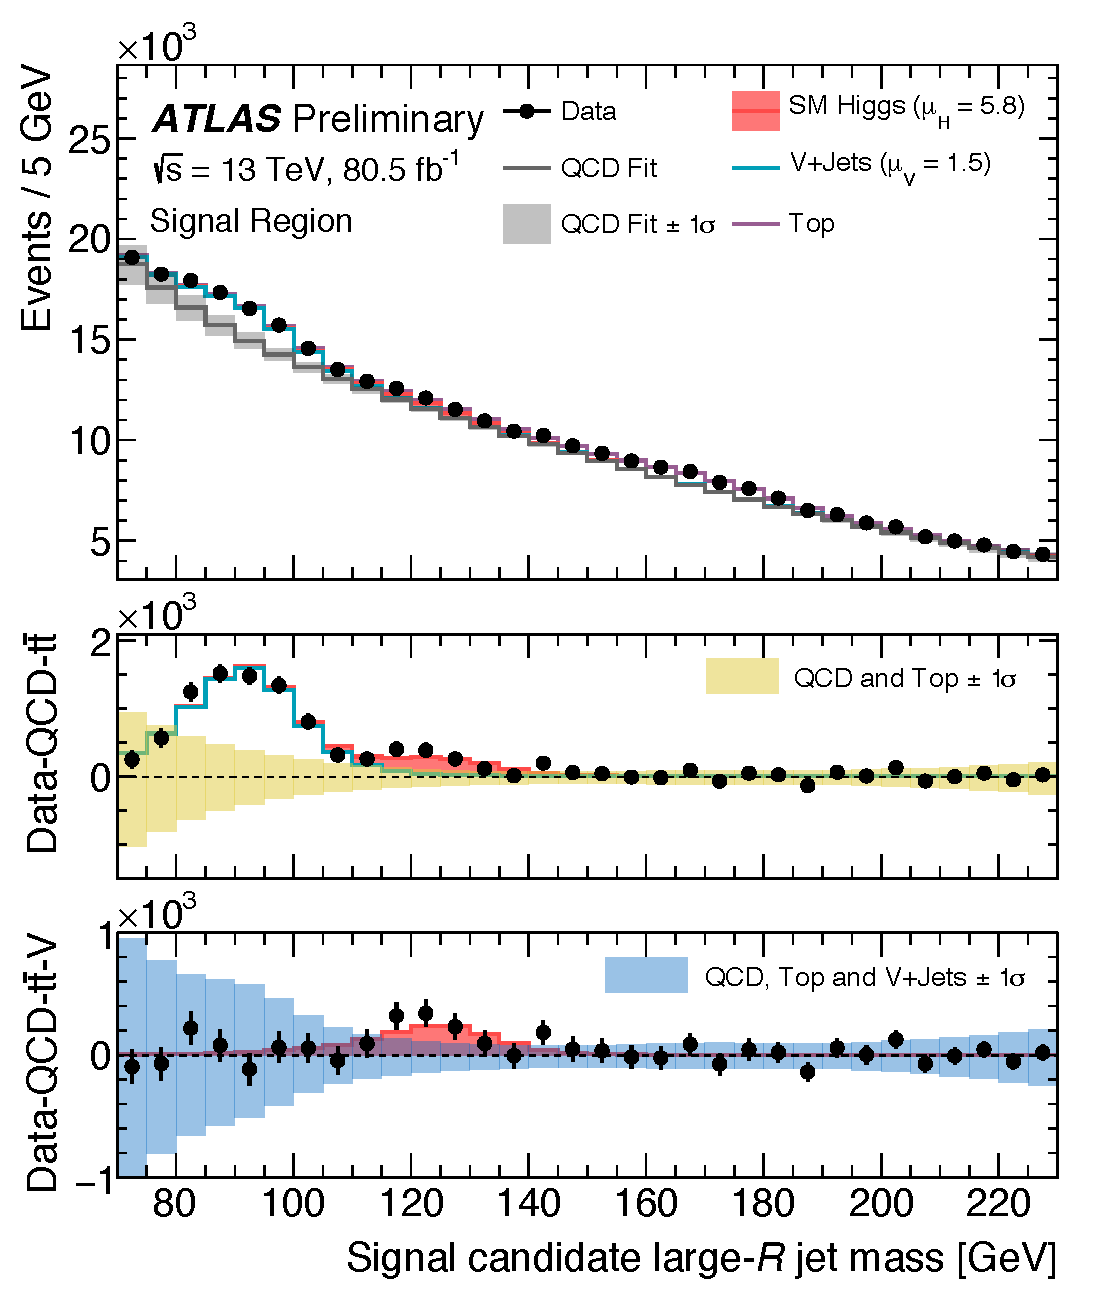
\includegraphics[width=\linewidth]{figures/results/money_plot}
\caption{ 
The top panel shows the post-fit comparison of the signal candidate large-$R$
jet mass distribution for the combined SM Higgs boson, $V$ + jets, $t\bar{t}$
and QCD model to the observed data \cite{ATLAS-CONF-2018-052}.  The middle
panel gives the ratio of the post-fit model and the data with the QCD and
$t\bar{t}$ components subtracted, highlighting the large resonance from $V$ +
jets.  The bottom panel gives the ratio of the post-fit model and the data with
the QCD, $V$ + jets, and $t\bar{t}$ components subtracted, highlighting a
slight excess of events near $m_{J} = 125~\GeV$.}
\label{sec:results:money_plot}
\end{figure}


\section{Observation of Boosted $V \rightarrow b\bar{b}$} \label{sec:results:v_jets}

The observed signal strength for the $V$ + jets process is:

$$ \mu_{V} = 1.5 \pm 0.22~\mathrm{(stat.)}^{+0.29}_{-0.25}~\mathrm{(syst.)} \pm 0.18~\mathrm{(th.)}\,, $$

corresponding to an observed significance of $5\sigma$ with an expected
significance of $4.8\sigma$ \Cite{Feickert:HiggsCouplings2018}.  This
measurement represents the first direct observation of boosted vector bosons
decaying to bottom quark pairs in ATLAS for $s = \sqrt{13}~\TeV$.

\section{Measurement of Boosted $H \rightarrow b\bar{b}$} \label{sec:results:procedure}

For the $H \rightarrow b\bar{b}$ process, the observed signal strength is:
%
$$ \mu_{H} = 5.8 \pm 3.1~\mathrm{(stat.)} \pm 1.9~\mathrm{(syst.)} \pm 1.7~\mathrm{(th.)}\,. $$
%
Given the uncertainties this result is consistent with the background-only
hypothesis at $1.6\sigma$ with an expected sensitivity of $0.28\sigma$
\cite{Feickert:HiggsCouplings2018}.  This constitutes a measurement of the
boosted Higgs decaying to a bottom quark pair but not a direct observation. The
result of the combined fit of the $V$ + jets and $H \rightarrow b\bar{b}$
signal models shows agreement with the Standard Model prediction of $\mu_{H} =
\mu_{V} = 1$ as seen in \Cref{sec:results:contour}.
%
\begin{figure}
\centering
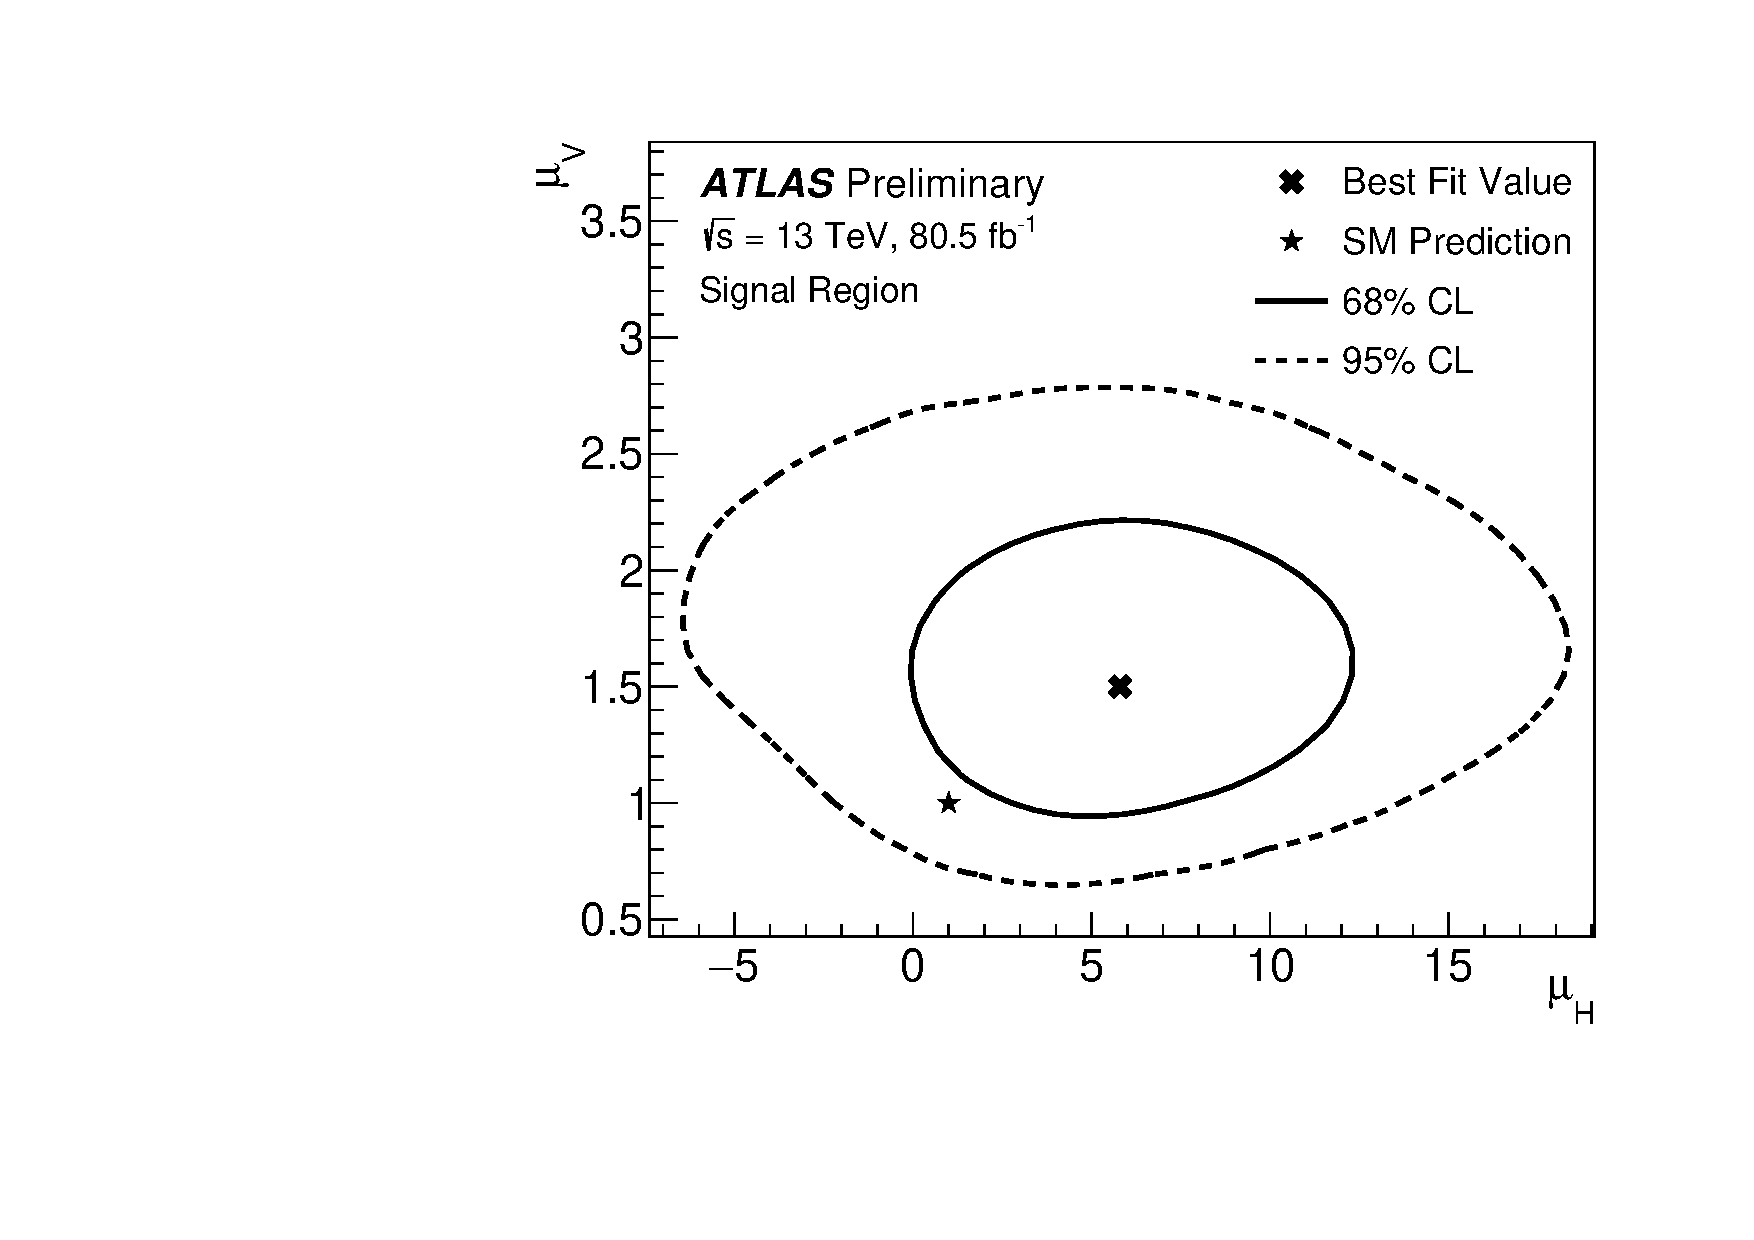
\includegraphics[width=.6\linewidth]{figures/results/contour}
\caption{\cite{ATLAS-CONF-2018-052}
Combined marginalized posterior distributions of $\mu_{H}$ and $\mu_{V}$ in the
Signal Region.  It is seen that the best-fit values for the signal processes
lie within the 68\% Credibility Level ($2\sigma$) of the Standard Model
prediction.}
\label{sec:results:contour}
\end{figure}



\part{Conclusion}
\chapter{Conclusion} \label{chap:conclusion}

I conclude that this secion is the conclusion


\addcontentsline{toc}{chapter}{Bibliography}
\printbibliography

\appendix

\chapter{Hadronic Vqq Sherpa Studies} \label{app:sherpa}


Ancillary material should be put in appendices, which appear after the
bibliography. 

\end{document}
